%% LaTeX2e class for student theses
%% sections/evaluation.tex
%% 
%% Karlsruhe Institute of Technology
%% Institute for Program Structures and Data Organization
%% Chair for Software Design and Quality (SDQ)
%%
%% Dr.-Ing. Erik Burger
%% burger@kit.edu
%%
%% Version 1.3.6, 2022-09-28

\chapter{Evaluation}
\label{ch:Evaluation}

In this section we will present the results of our experiments. As mentioned before, our experiments are split into two parts. The first part is the evaluation of our novel
Continual Active Learning Approach and the second part is evaluating the performance our the Continual Active Learning approach when applied to Model Stealing. In each of these
respective subsections we will first describe the experiments schedule for each part and then present the results of the experiments.



\section{Continual Active Learning}
\label{sec:CAL}
In this subsection we will first present the results of running all combinations of the Active Learning strategies \gls{bald},\gls{badge},CoreSet,\gls{lc} and Random with the Continual Learning strategies
Naive, \gls{ewc}, \gls{mas}, \gls{alasso} and \gls{imm}. Afterwards, we will analyze the behavior of a hybrid approach between Active Learning and Continual Active Learning, where we first run a few cycles with
pure Active Learning before switching to Continual Active Learning. We further analyze the performance of different strategies to initialize the labeled pool. Next, we experiment with \gls{vaal}
and \gls{a-gem}.

\subsubsection{Combining Active Learning and Regularization-based Continual Learning}
\label{sec:Evaluation:Results:CAL:ALRegCL}
To evaluate the combination of the Active Learning strategies \gls{bald},\gls{badge},Coreset,\gls{lc} and Random with the Continual Learning strategies Naive, \gls{ewc}, \gls{mas}, \gls{alasso} and \gls{imm}, we run each combination
using a batch size of 1000,2000 and 4000. We use the CIFAR-10 dataset and the Neural Network Architecture Resnet18 for these experiments. We present the validation accuracy with increasing
size of the labeled pool as well as the overall runtime of each experiment. \par
In figure \ref{fig:Evaluation:Results:CAL:Random1000} we present the results of running the Active Learning strategy Random with the Continual Learning strategies Naive, \gls{ewc}, \gls{mas}, \gls{alasso} and \gls{imm}
as well as the baseline of running pure Active Learning. We use a batch size of 1000 for these experiments. In terms of runtime, all strategies are significantly faster than the classic Active
Learning approach. \gls{mas}, \gls{imm}, \gls{ewc} and Naive all are approximately 50 times as fast as the classic Active Learning approach. \gls{alasso} is slightly slower than the other Continual Learning strategies,
but still about 25 times faster than the baseline. However, there is a notable gap in validation accuracy between Active Learning and all Continual Active Learning strategies. \gls{imm} is the only
Continual Learning strategy to outperform the Naive approach. \gls{ewc} performs slightly worse Naive while \gls{mas} and \gls{alasso} perform significantly worse. While the validation accuracy of \gls{mas} increases only
slightly with an increasing size of the labeled pool, \gls{alasso} has an erratic validation curve which does not seem to stabilize until the end of the experiment. \par
\begin{figure}[h]
    \centering
    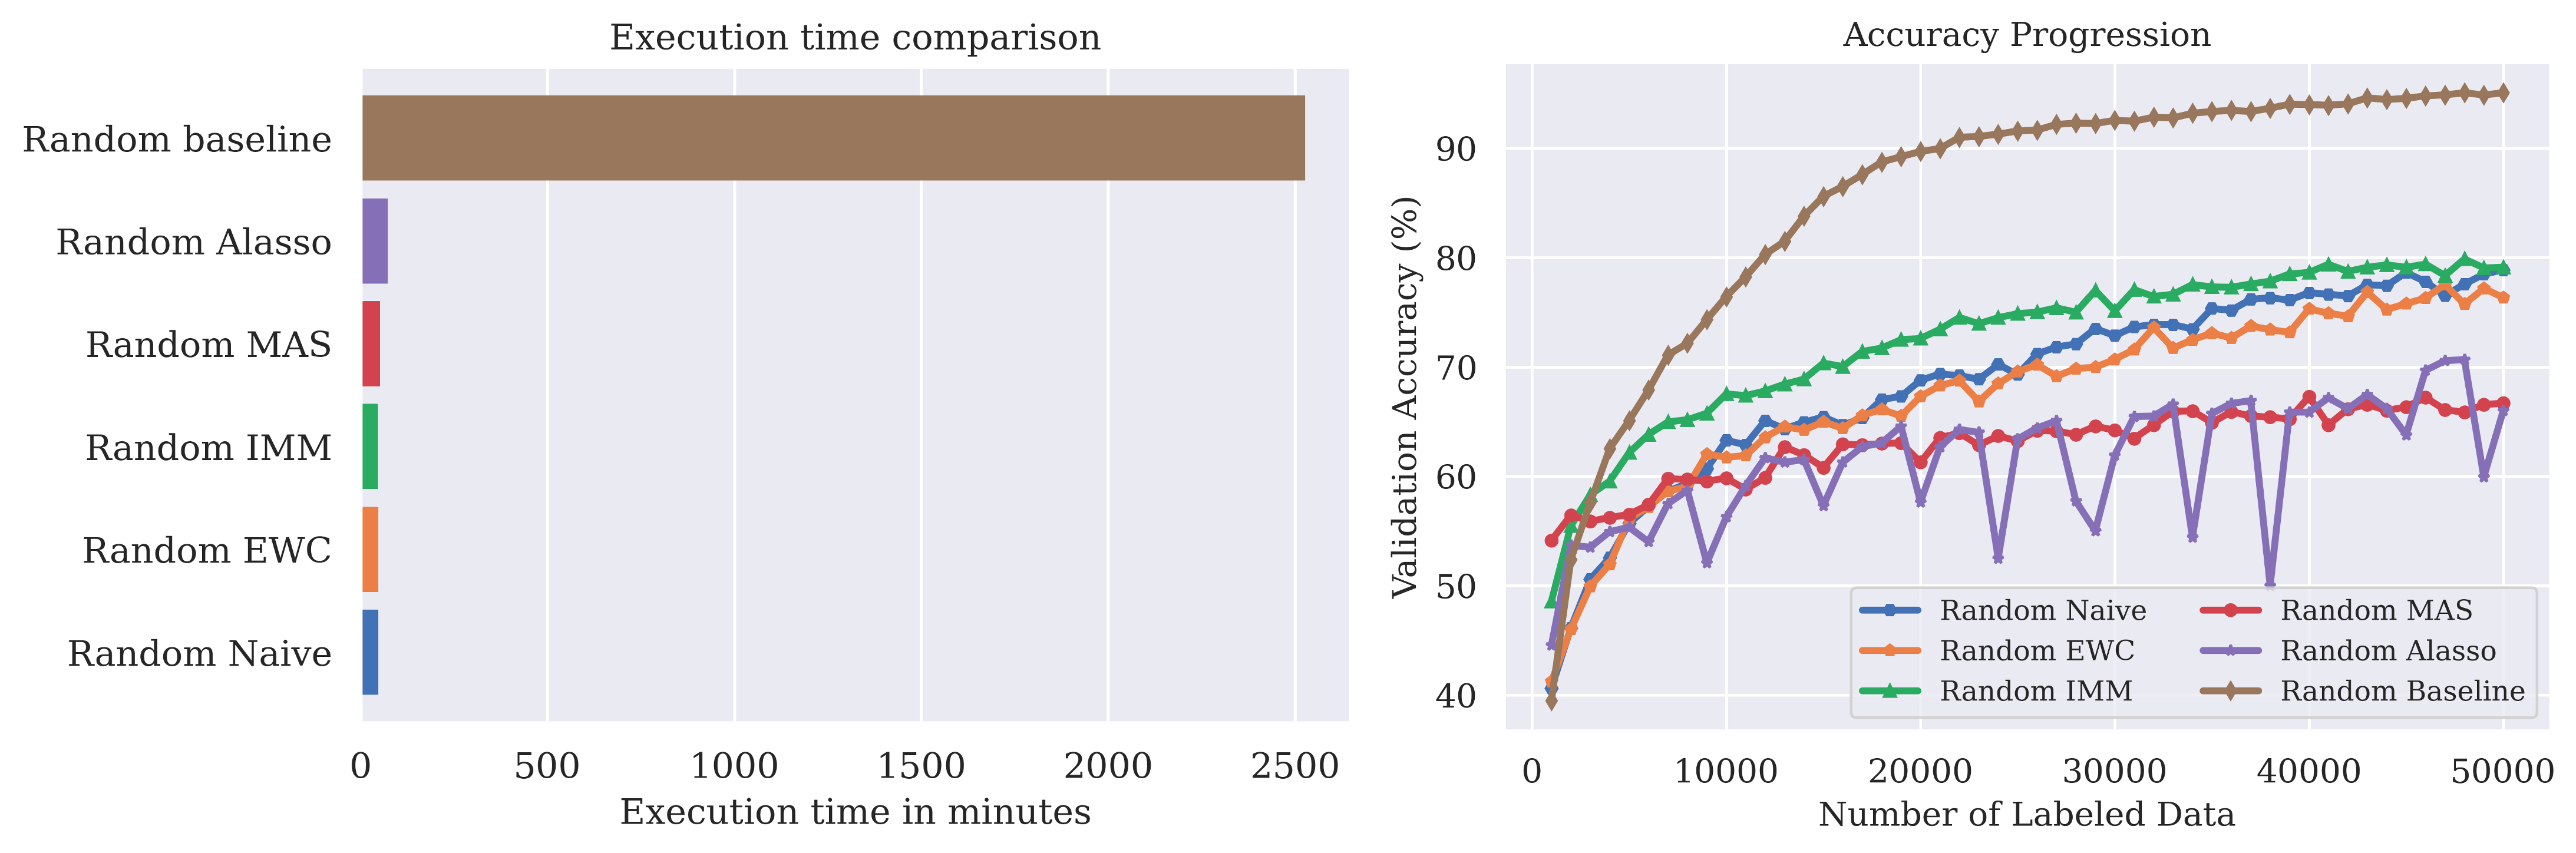
\includegraphics[width=\linewidth]{images/results_CAL/Random_CAL_1000b.png}
    \caption[Continual Active Learning Random 1000 batch size]{Comparison of execution time and validation accuracy of Continual Learning strategies used with the Active Learning strategy random.
    We use a batch size of 1000 for the experiments.}
    \label{fig:Evaluation:Results:CAL:Random1000}
\end{figure}

Next, we run the same experiment setup with the Active Learning strategy \gls{lc}. Results can be found in figure \ref{fig:Evaluation:Results:CAL:LC1000}. Again, all Continual Learning strategies
are significantly outperform the baseline in terms of execution time. \gls{alasso} is the slowest Continual Learning strategy, albeit being roughly 25 times faster than the baseline. The remaining Continual
Learning strategies, \gls{imm}, \gls{mas}, CoreSet and \gls{ewc}, are all about 50 times faster than the baseline. The gap in validation accuracy between Active Learning and all Continual Active Learning strategies
remains similar to the gap observed with Random. \gls{imm} and Naive perform similarly, outperforming the remaining Continual Learning strategies in the first half of the experiment. \gls{ewc} picks up on their
performance in the after 25000 sampled data. \gls{mas} and \gls{alasso} fall behind in terms of performance, with \gls{alasso} experiencing significant accuracy drops. \gls{mas}' validation accuracy remain stable throughout
the whole experiment, catching up to the other Continual Learning strategies in the end. \par

\begin{figure} [h]
    \centering
    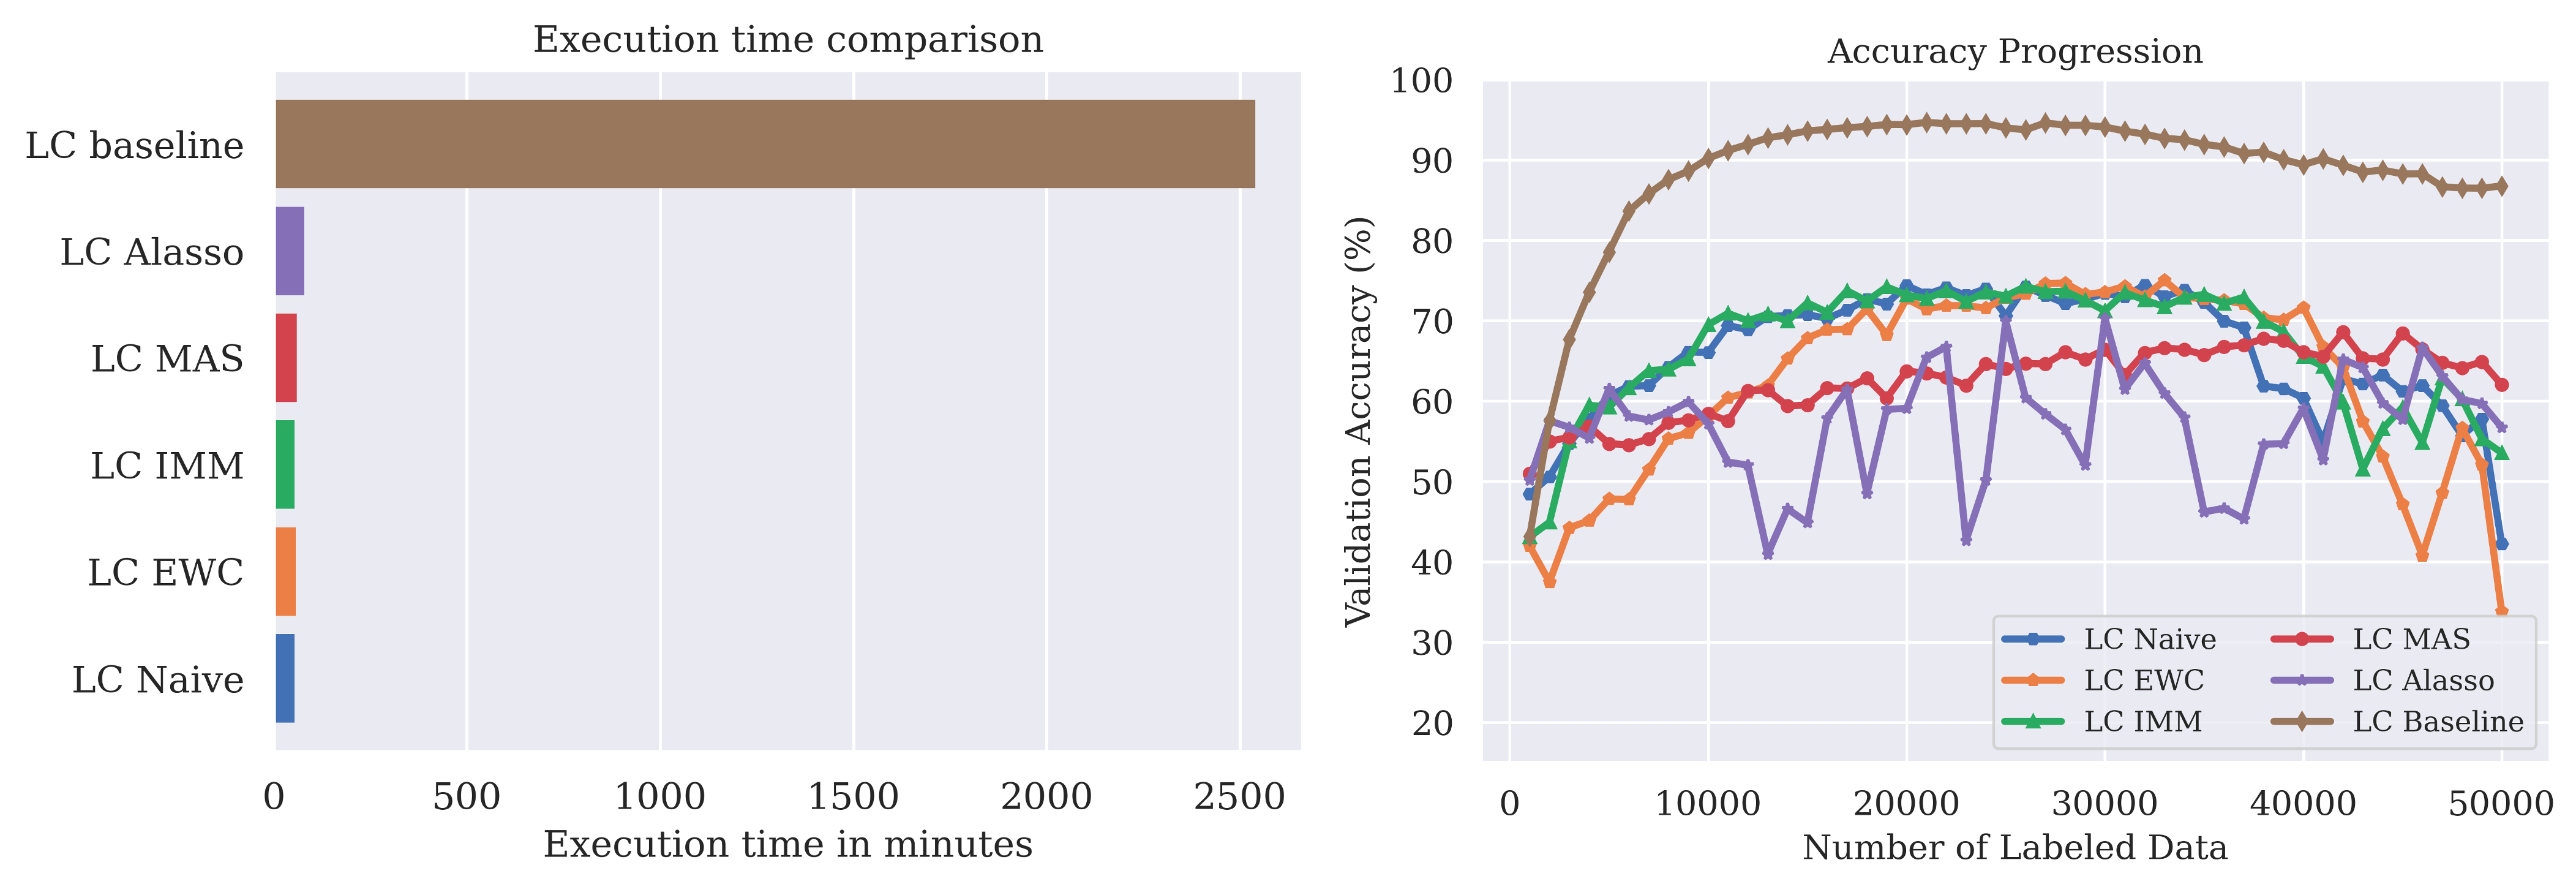
\includegraphics[width=\linewidth]{images/results_CAL/LC_CAL_1000b.png}
    \caption[Continual Active Learning \gls{lc} 1000 batch size]{Comparison of execution time and validation accuracy of Continual Learning strategies used with the Active Learning strategy \gls{lc}.
    We use a batch size of 1000 for the experiments.}
    \label{fig:Evaluation:Results:CAL:LC1000}
\end{figure}

\gls{bald} is the third Active Learning strategy we evaluate. Again, we use the same experiments setup as in the previous two experiments, changing only the Active Learning strategy but leaving every-
thing else as-is. The results of these experiments can be found in figure \ref{fig:Evaluation:Results:CAL:BALD1000}. In terms of runtime, the pattern established using \gls{lc} and Random continues.
\gls{mas}, \gls{imm}, \gls{ewc} and Naive are approximately 50 times as fast as the baseline, while \gls{alasso} is about 25 times as fast. Considering validation accuracy, all Continual Learning strategies perform significantly
worse than the baseline. Establishing a ranking between the Continual Learning strategies is difficult however, because they are all very erratic. \gls{alasso} stands out with the best and worst validation
accuracy, depending on the number of labeled samples. \gls{imm}, \gls{mas}, Naive and \gls{ewc} all have similar validaiton accuracy curves, although they are less erratic than \gls{alasso}. \par

\begin{figure}[h]
    \centering
    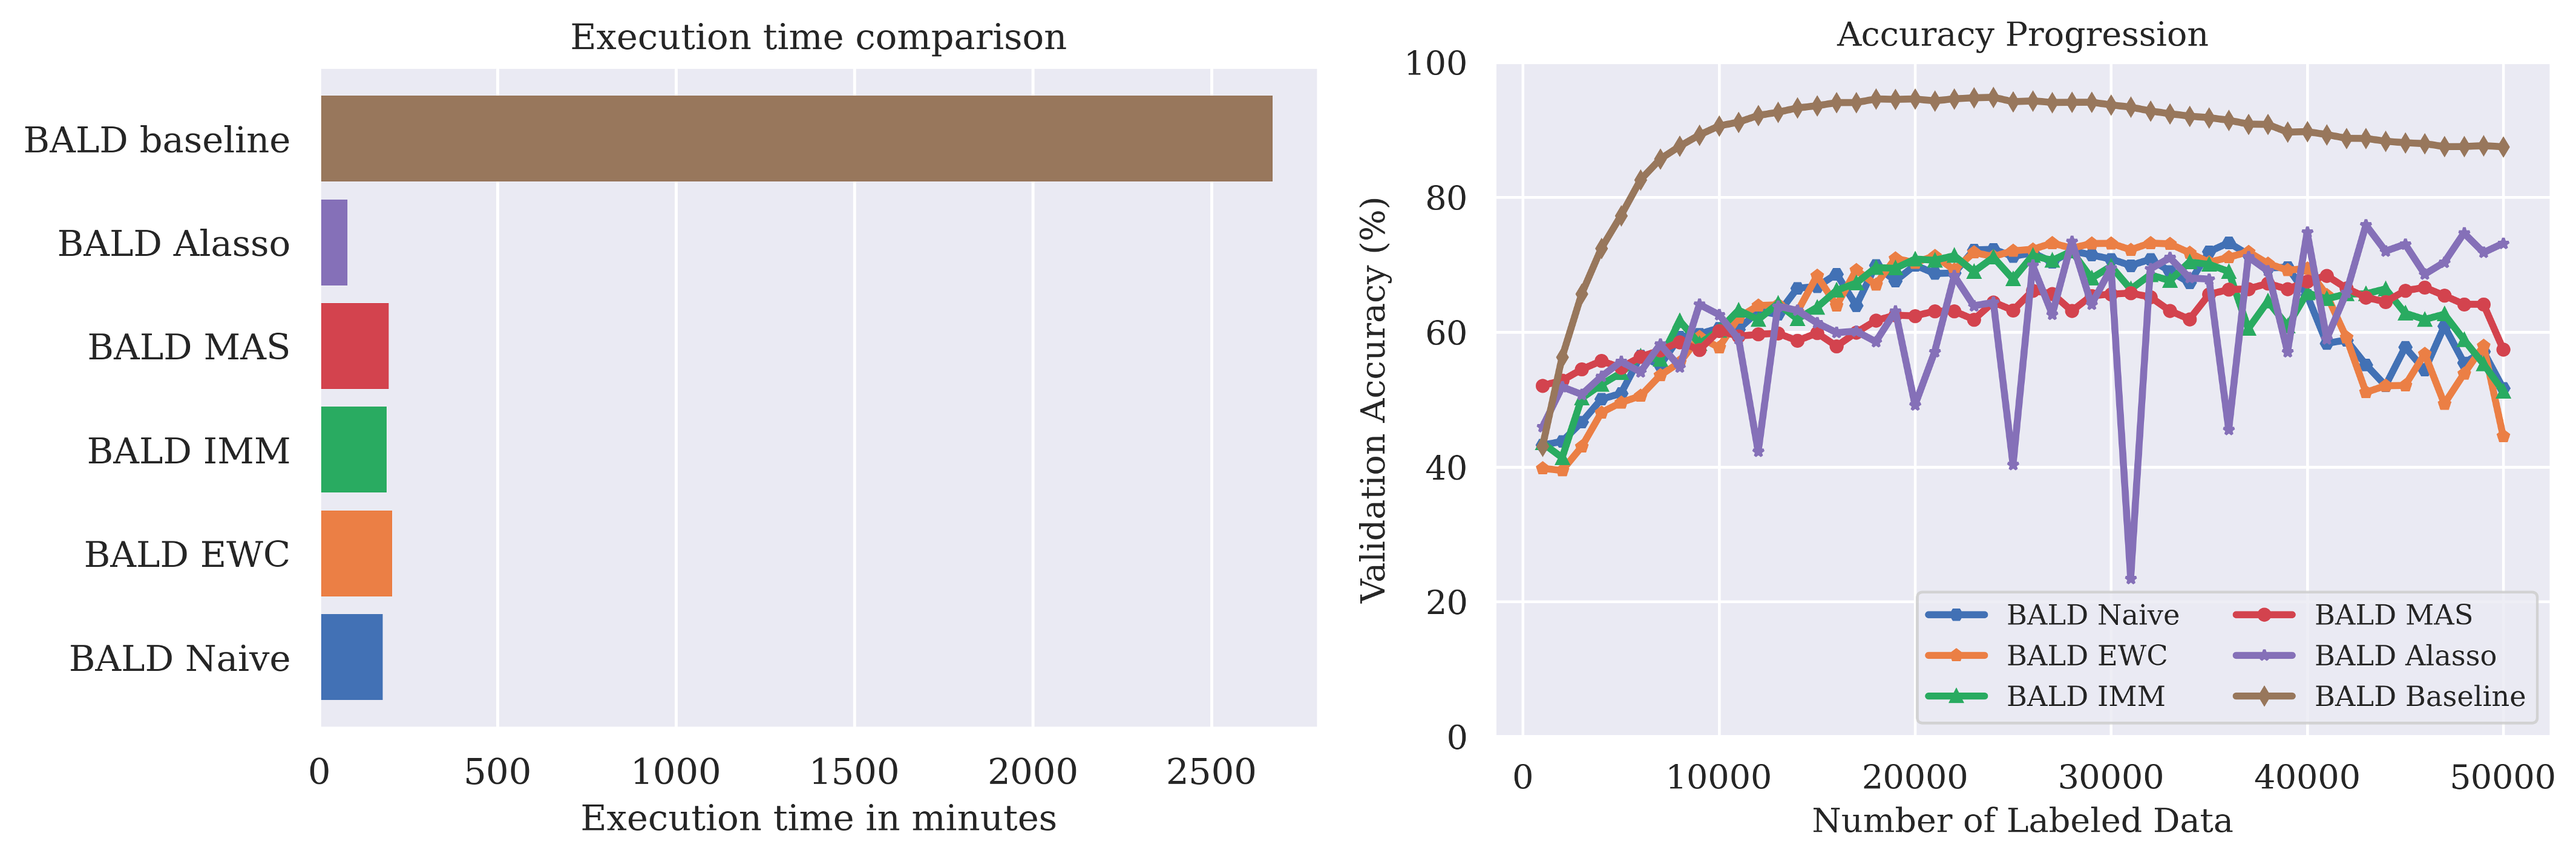
\includegraphics[width=\linewidth]{images/results_CAL/Bald_CAL_1000b.png}
    \caption[Continual Active Learning \gls{bald} 1000 batch size]{Comparison of execution time and validation accuracy of Continual Learning strategies used with the Active Learning strategy \gls{bald}.
    We use a batch size of 1000 for the experiments.}
    \label{fig:Evaluation:Results:CAL:BALD1000}
\end{figure}

After running our experiment with \gls{bald}, we re-run it using the Active Learning strategy CoreSet. We present the results in figure \ref{fig:Evaluation:Results:CAL:CoreSet1000}. The runtime of the 
Continual Learning strategies is again significantly lower than that of the baseline, however it is higher than in the previous experiments. \gls{alasso} is the slowest Continual Learning strategy, being
around 12 times as fast as the baseline. \gls{imm}, \gls{mas}, \gls{ewc} and Naive have a similar execution time and are approximately 15 times as fast as Active Learning using CoreSet. Just as in the previous experiments,
there is a significant gap in validation accuracy between the baseline and all Continual Learning strategies. \gls{imm}, \gls{ewc} and Naive perform almost similarly while \gls{mas} and \gls{alasso} fall behind. While \gls{mas} demon-
strates a marginally increasing validation accuracy, the validation accuracy curve of \gls{alasso} is unstable with significant drops and jumps in accuracy as the number of labeled data increases. \par

\begin{figure}[h]
    \centering
    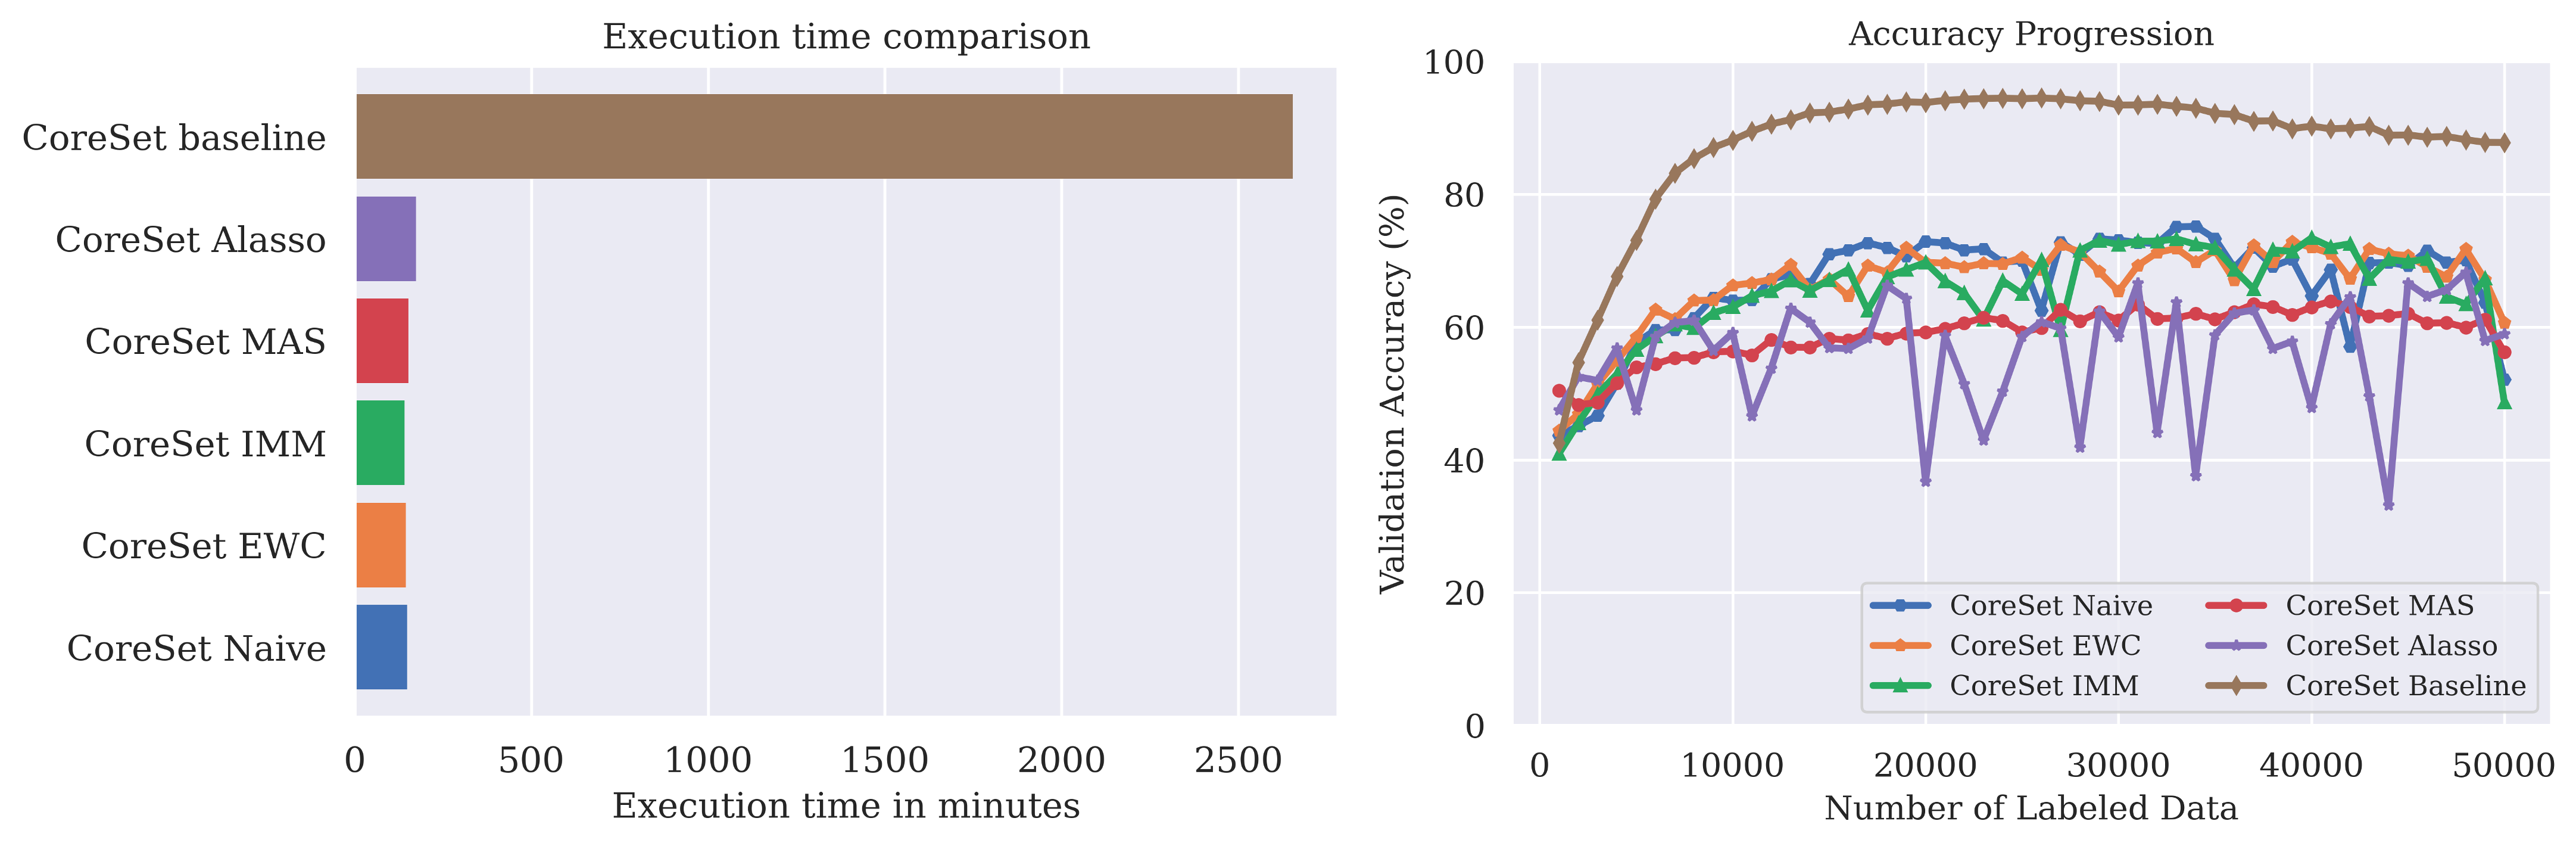
\includegraphics[width=\linewidth]{images/results_CAL/CoreSet_CAL_1000b.png}
    \caption[Continual Active Learning CoreSet 1000 batch size]{Comparison of execution time and validation accuracy of Continual Learning strategies used with the Active Learning strategy
     CoreSet. We use a batch size of 1000 for the experiments. }
    \label{fig:Evaluation:Results:CAL:CoreSet1000}
\end{figure}

In our final experiment with batch size 1000, we use the Active Learning strategy \gls{badge}. The results are shown in figure \ref{fig:Evaluation:Results:CAL:Badge1000}. All Continual Learning strategies
outperform the baseline in terms of runtime by a large margin. Between the Continual Learning strategies, there are only marginal differences in execution time. The validation accuracy of all Continual
Learning strategies is irregular and all of them leave a significant gap to the baseline. There is no Continual Learning strategy which demonstrates a significantly higher or lower validation accuracy
than the others. However, \gls{mas} and \gls{alasso} fall behind the other Continual Learning strategies at around 25000 samples but manage to catch up in the end. \par

\begin{figure}[h]
    \centering
    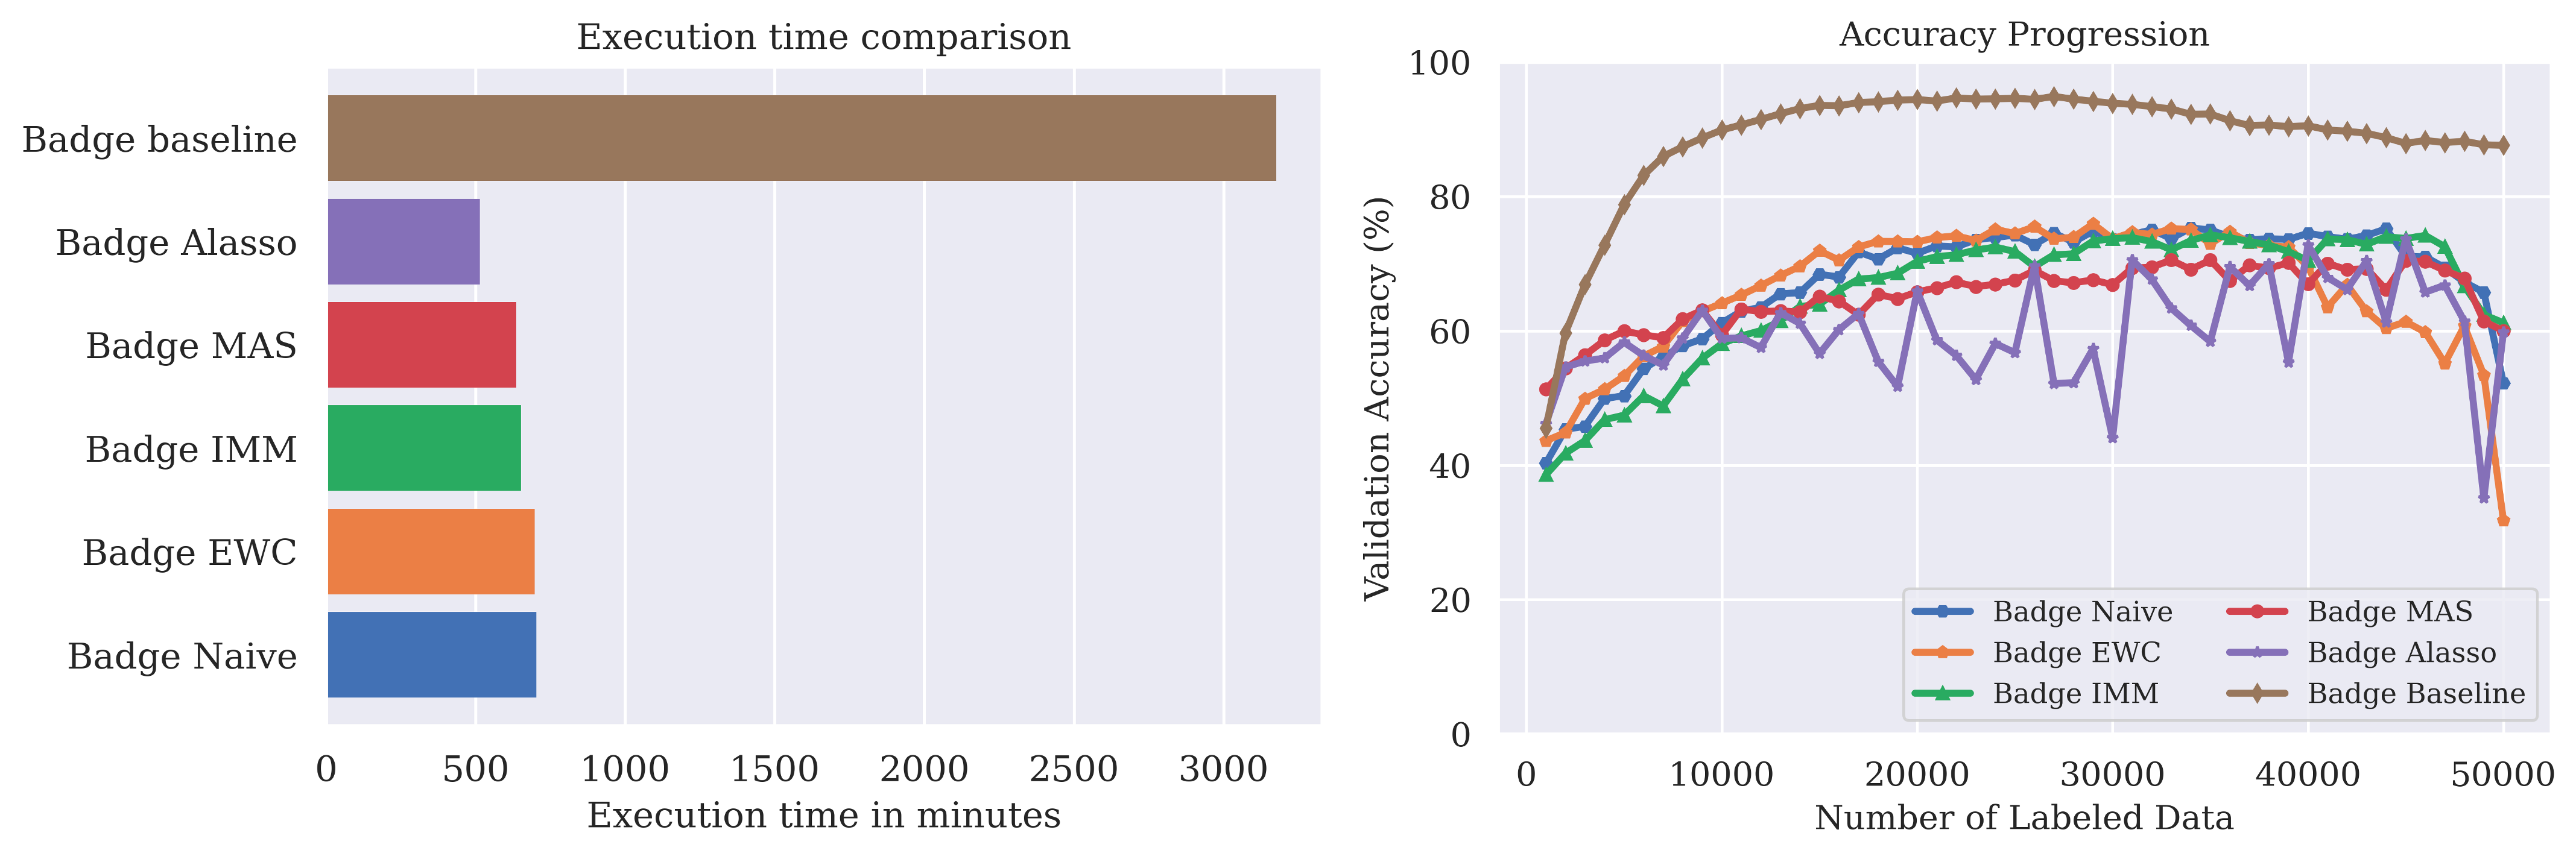
\includegraphics[width=\linewidth]{images/results_CAL/Badge_CAL_1000b.png}
    \caption[Continual Active Learning \gls{badge} 1000 batch size]{Comparison of execution time and validation accuracy of Continual Learning strategies used with the Active Learning strategy
    \gls{badge}. We use a batch size of 1000 for the experiments. }
    \label{fig:Evaluation:Results:CAL:Badge1000}
\end{figure}

After running the experiment with \gls{badge}, CoreSet, \gls{lc}, \gls{bald} and Random, we perform the same experiment with Random but increase the batch size from 1000 to 2000. We present the results in
Figure \ref{fig:Evaluation:Results:CAL:Random2000}. The execution time remains significantly lower for all Continual Learning strategies compared to the baseline, however, the gap has decreased. 
\gls{alasso} is the slowest Continual Learning Strategy, being about 8 times as fast as the baseline. \gls{mas}, \gls{imm}, \gls{ewc} and Naive have similar execution times, being about 10 times as fast as the baseline. 
The gap in validation accuracy between the baseline and the Continual Learning strategies is still significant, however, it has decreased compared the experiment with a batch size of 1000.
\gls{ewc} outperforms all Continual Learning strategies, including Naive, although the gap between the two is marginal. \gls{alasso}, \gls{imm} and \gls{mas} perform show similar overall performance although the course
of their validation accuracy curves differ greatly. \gls{imm} starts worst and ends best. \gls{mas} shows similar performance to \gls{alasso} but is outperformed within the final 5000 samples. \par

\begin{figure}[h]
    \centering
    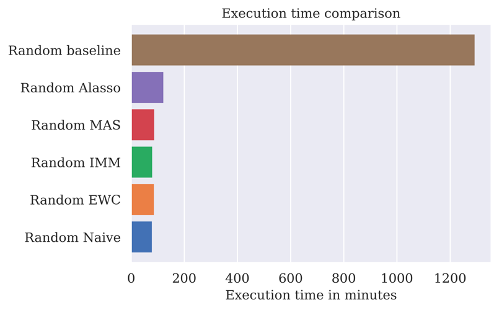
\includegraphics[width=\linewidth]{images/results_CAL/Random_CAL_2000b.png}
    \caption[Continual Active Learning Random 2000 batch size]{Comparison of execution time and validation accuracy of Continual Learning strategies used with the Active Learning strategy
    Random. We use a batch size of 2000 for the experiments.}
    \label{fig:Evaluation:Results:CAL:Random2000}
\end{figure}

Second, we run the experiment with batch size 2000 for the Active Learning strategy \gls{lc}. Our results can be found in figure \ref{fig:Evaluation:Results:CAL:LC2000}. Like in the previous experiment,
the gap in execution time between the baseline and the Continual Learning strategies has shrunk compared to the experiment with a batch size of 1000. Again, \gls{alasso} is the slowest Continual Learning
strategy, being approximately 9 times as fast as the baseline. \gls{ewc} is the second slowest strategy, being only marginally slower than \gls{mas}, \gls{imm} and Naive, who have a very similar execution time.
In terms of validation accuracy, there is still a significant gap between the baseline and the Continual Learning strategies. \gls{imm}, \gls{ewc} and Naive perform similar for the first 35000 samples, outperforming
\gls{mas} and \gls{alasso}. In the final 15000 samples, all \gls{imm}, \gls{ewc} and Naive experience a drop in validation accuracy, which is most significant for \gls{ewc}. The accuracy of \gls{mas} increases modestly until the labeled
pool contains 40000 samples, before dropping of by about 10\%. The validation accuracy curve of \gls{alasso} is again unstable, showing a slight downward trend over the course of the experiment. \par

\begin{figure}[h]
    \centering
    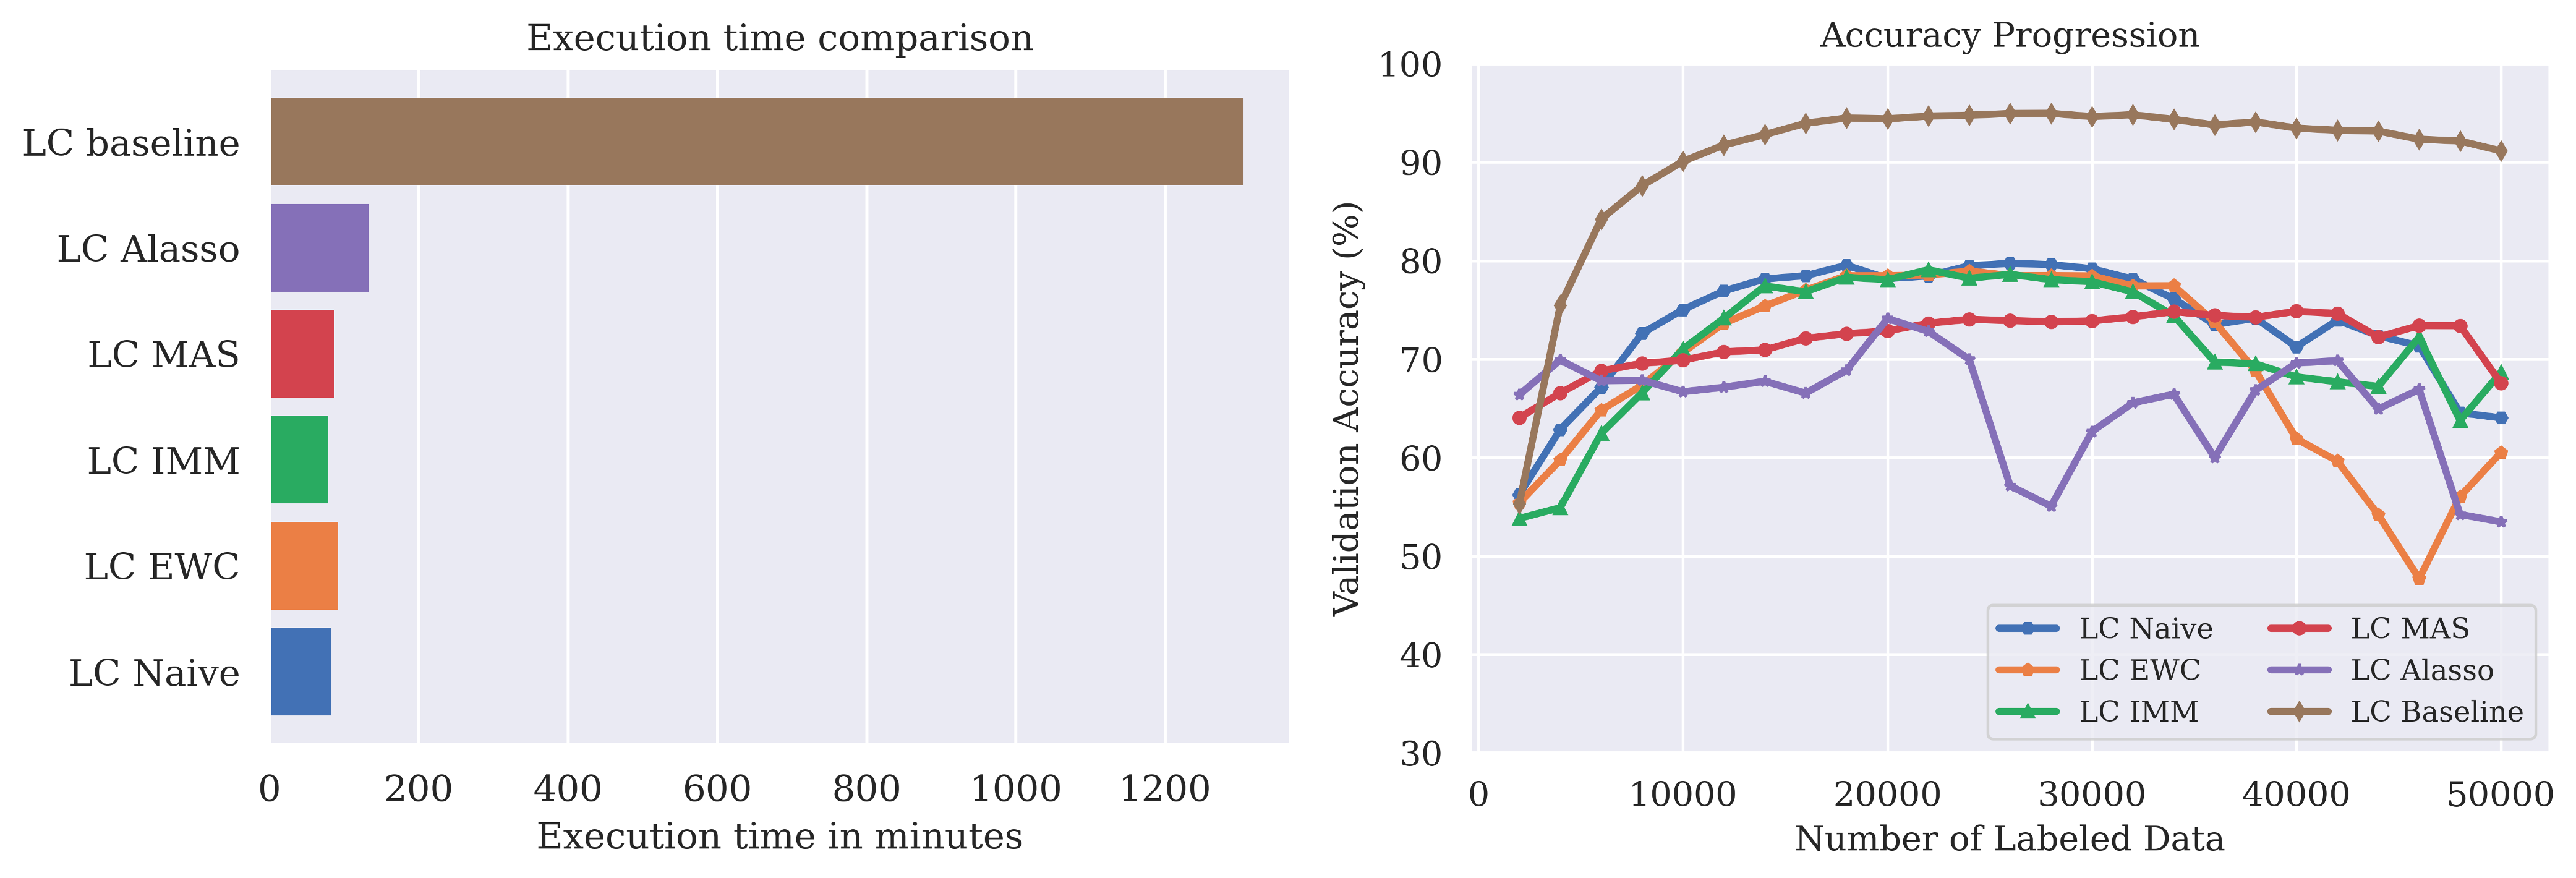
\includegraphics[width=\linewidth]{images/results_CAL/LC_CAL_2000b.png}
    \caption[Continual Active Learning \gls{lc} 2000 batch size]{Comparison of execution time and validation accuracy of Continual Learning strategies used with the Active Learning strategy
    \gls{lc}. We use a batch size of 2000 for the experiments.}
    \label{fig:Evaluation:Results:CAL:LC2000}
\end{figure}

We follow up with the experiment using the Active Learning strategy \gls{bald}, all other parameters being equal. The results can be found in figure \ref{fig:Evaluation:Results:CAL:BALD2000}. The gap in
execution time between the baseline and the Continual Learning strategies has declined compared to the experiment with \gls{bald} and batch size 1000. Naive and \gls{imm} are the fastest Continual Learning strategies,
closely followed \gls{ewc} and \gls{mas}. \gls{alasso} follows last, but is still about 10 times as fast as the baseline. The validation accuracy curves of most Continual Learning strategies are similar, with \gls{alasso} falling 
out of line. \gls{ewc}, \gls{imm} and Naive perform similar across the whole experiment with \gls{mas} starting off better but falling behind after approximately 15000 samples. \gls{alasso} performs on par with the remaining strategies
at first, but suffers from a heavy decrease in validation accuracy at around 15000 samples. All Continual Learning strategies leave a large gap to the baseline in terms of validation accuracy. \par

\begin{figure}[h]
    \centering
    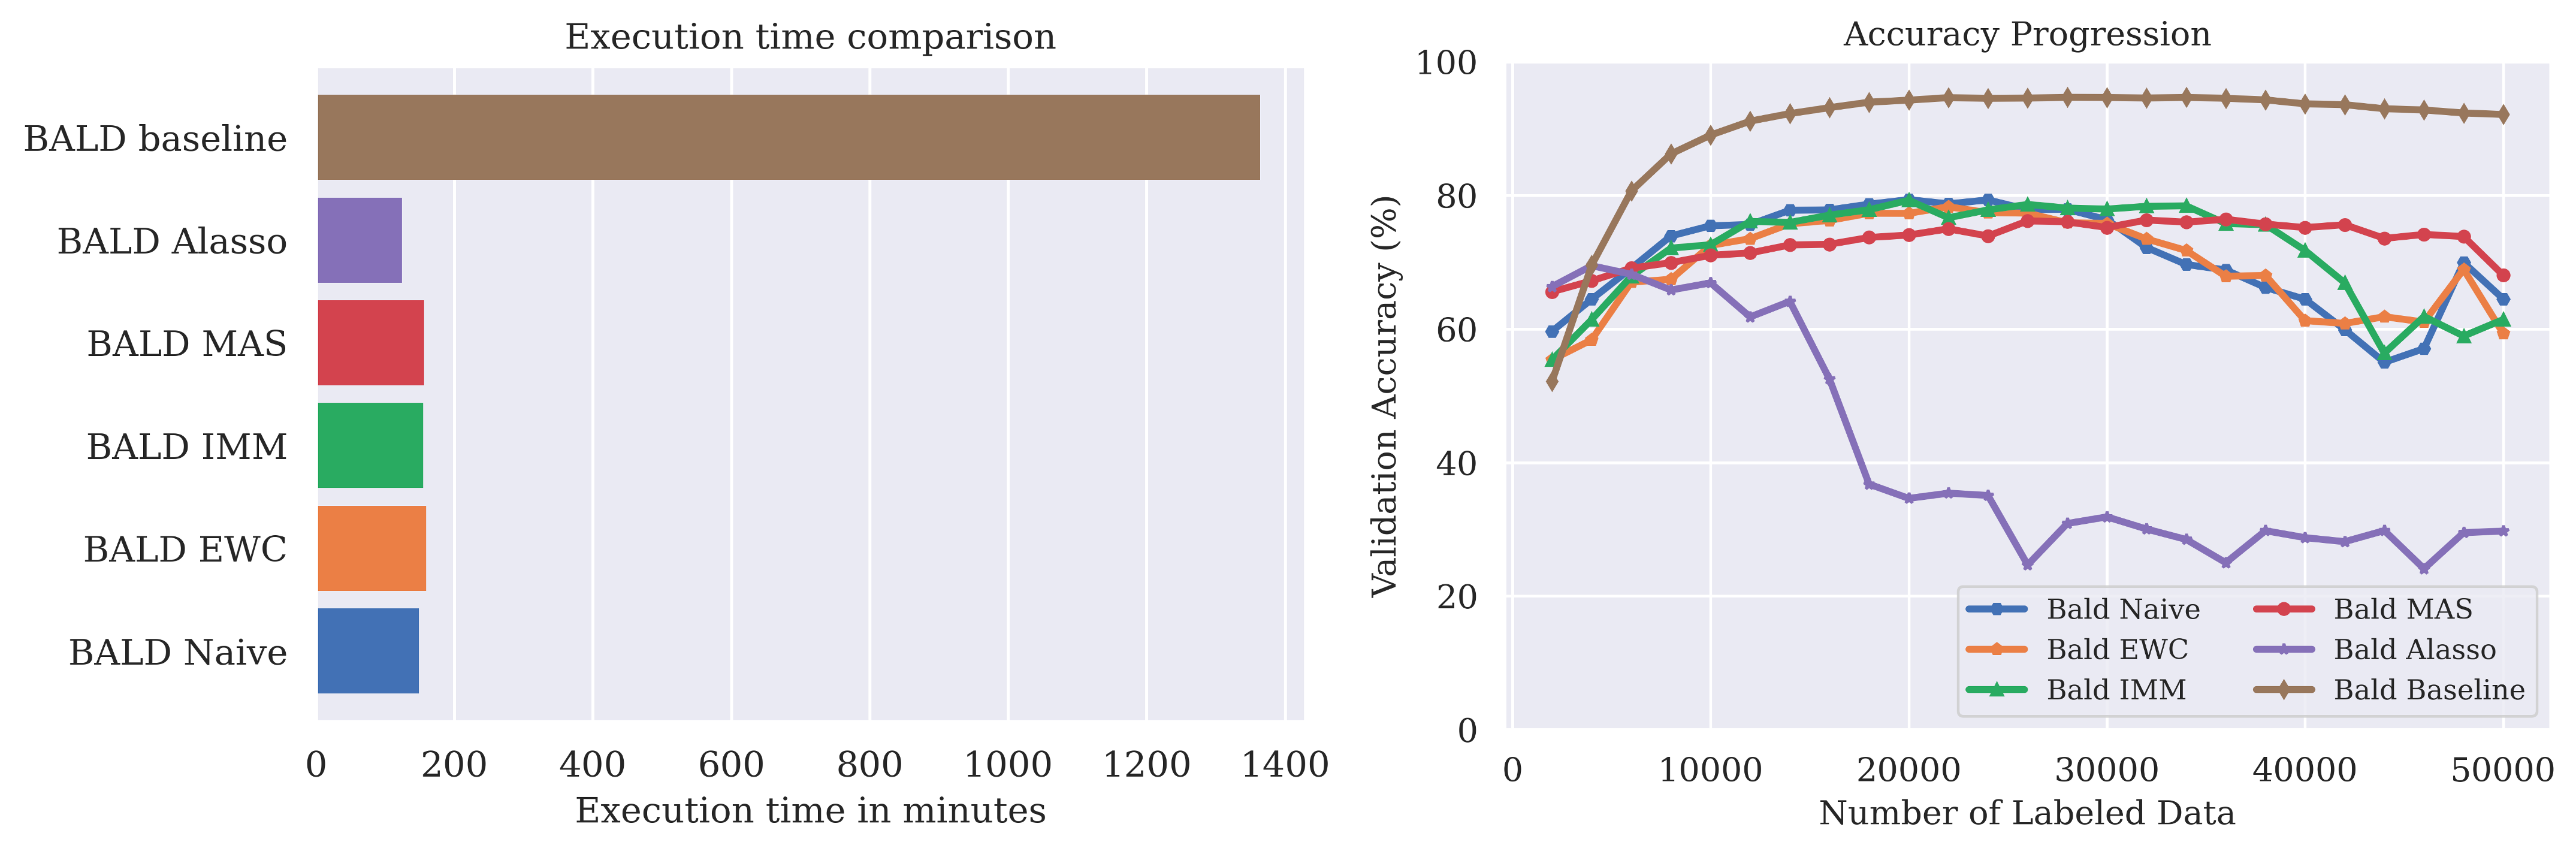
\includegraphics[width=\linewidth]{images/results_CAL/Bald_CAL_2000b.png}
    \caption[Continual Active Learning \gls{bald} 2000 batch size]{Comparison of execution time and validation accuracy of Continual Learning strategies used with the Active Learning strategy
    \gls{bald}. We use a batch size of 2000 for the experiments.}
    \label{fig:Evaluation:Results:CAL:BALD2000}
\end{figure}

Next, we run the experiment with CoreSet and a batch size of 2000. We present our results in figure \ref{fig:Evaluation:Results:CAL:CoreSet2000}. The gap in execution time between the baseline and the
Continual Learning strategies has again decreased. \gls{imm} is the fastest Continual Learning strategy, closely followed by \gls{ewc}. \gls{ewc} is followed by Naive and \gls{mas}, who have similar execution times. \gls{alasso} is
the slowest approach, albeit being about 6.5 times as fast as the baseline. Regarding validation accuracy, all Continual Learning strategies are significantly outperformed by the baseline. Naive performs best
in the first half of the experiment, followed by \gls{ewc}, \gls{imm} and \gls{mas}. At around 25000 samples, the validation accuracy of \gls{imm}, \gls{ewc} and Naive suddenly becomes erratic, followed by a moderate increase in validation
accuracy and a drop in the final 10000 samples. \gls{mas} performs consistent but worse than \gls{imm}, \gls{ewc} and Naive, experiencing a moderate drop in validation accuracy in the final 10000 samples. \gls{alasso} performs worst,
with its validation accuracy decreasing over the course of the experiment. \par

\begin{figure}[h]
    \centering
    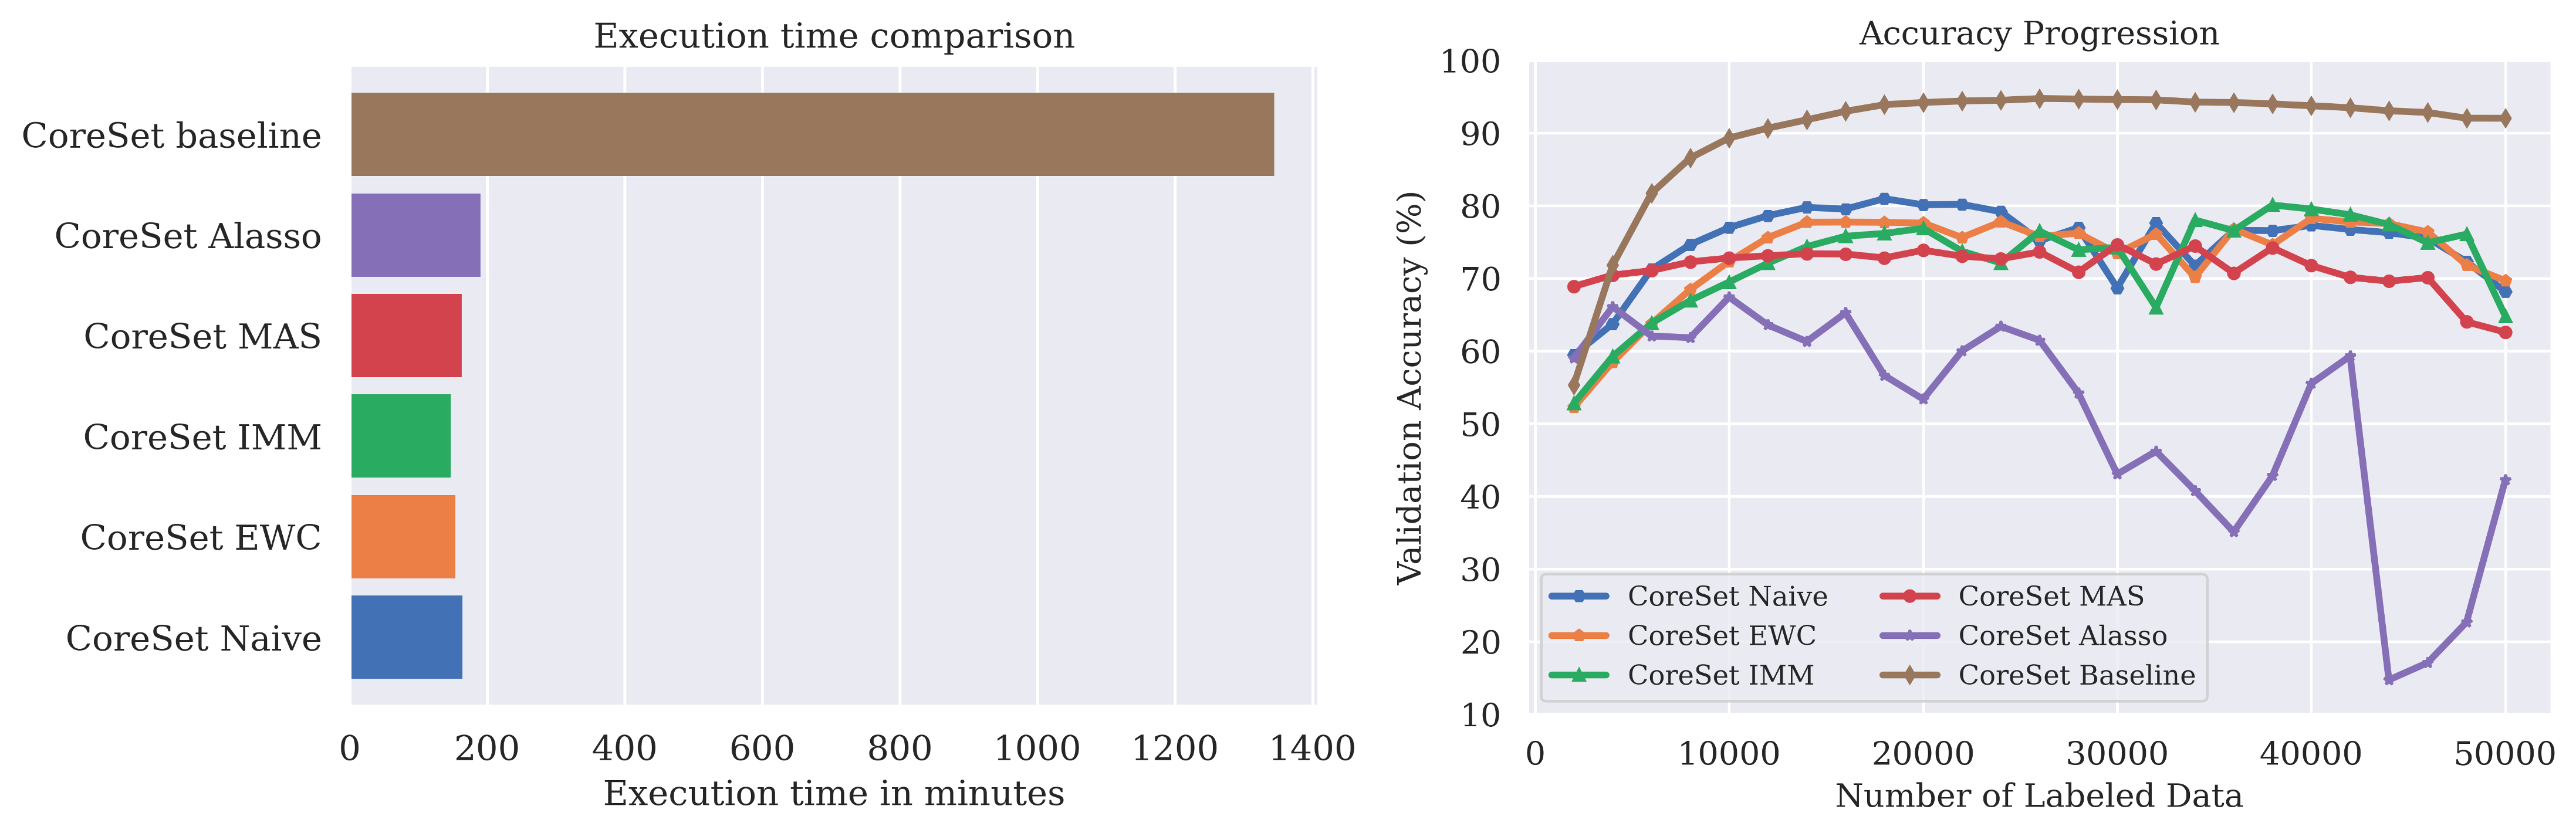
\includegraphics[width=\linewidth]{images/results_CAL/CoreSet_CAL_2000b.png}
    \caption[Continual Active Learning CoreSet 2000 batch size]{Comparison of execution time and validation accuracy of Continual Learning strategies used with the Active Learning strategy
    CoreSet. We use a batch size of 2000 for the experiments.}
    \label{fig:Evaluation:Results:CAL:CoreSet2000}
\end{figure}

Finally, we run the same experiment with the Active Learning strategy \gls{badge}. Our results can be found in figure \ref{fig:Evaluation:Results:CAL:Badge2000}. The margin in execution time between the baseline
and the Continual Learning strategies has decreased which is mainly due to the large decrease in runtime of the baseline, compared to the experiment with 1000 batch size. Nevertheless, the Continual
Learning strategies are about 3.5 times as fast as the baseline. Within the Continual Learning strategies there is only a minor runtime difference, with \gls{imm} being the fastest and \gls{alasso} the slowest. In terms of 
validation accuracy, the gap between the baseline as the Continual Learning strategies has decreased. More notably though, the validation accuracy curves of all Continual Learning strategies more consistent than
in the previous experiment with 1000 batch size. \gls{imm}, \gls{ewc} and Naive perform similar, followed by \gls{mas}. \gls{alasso} is the worst performing strategy, falling behind the others after bout 10000 samples. \par

\begin{figure}[h]
    \centering
    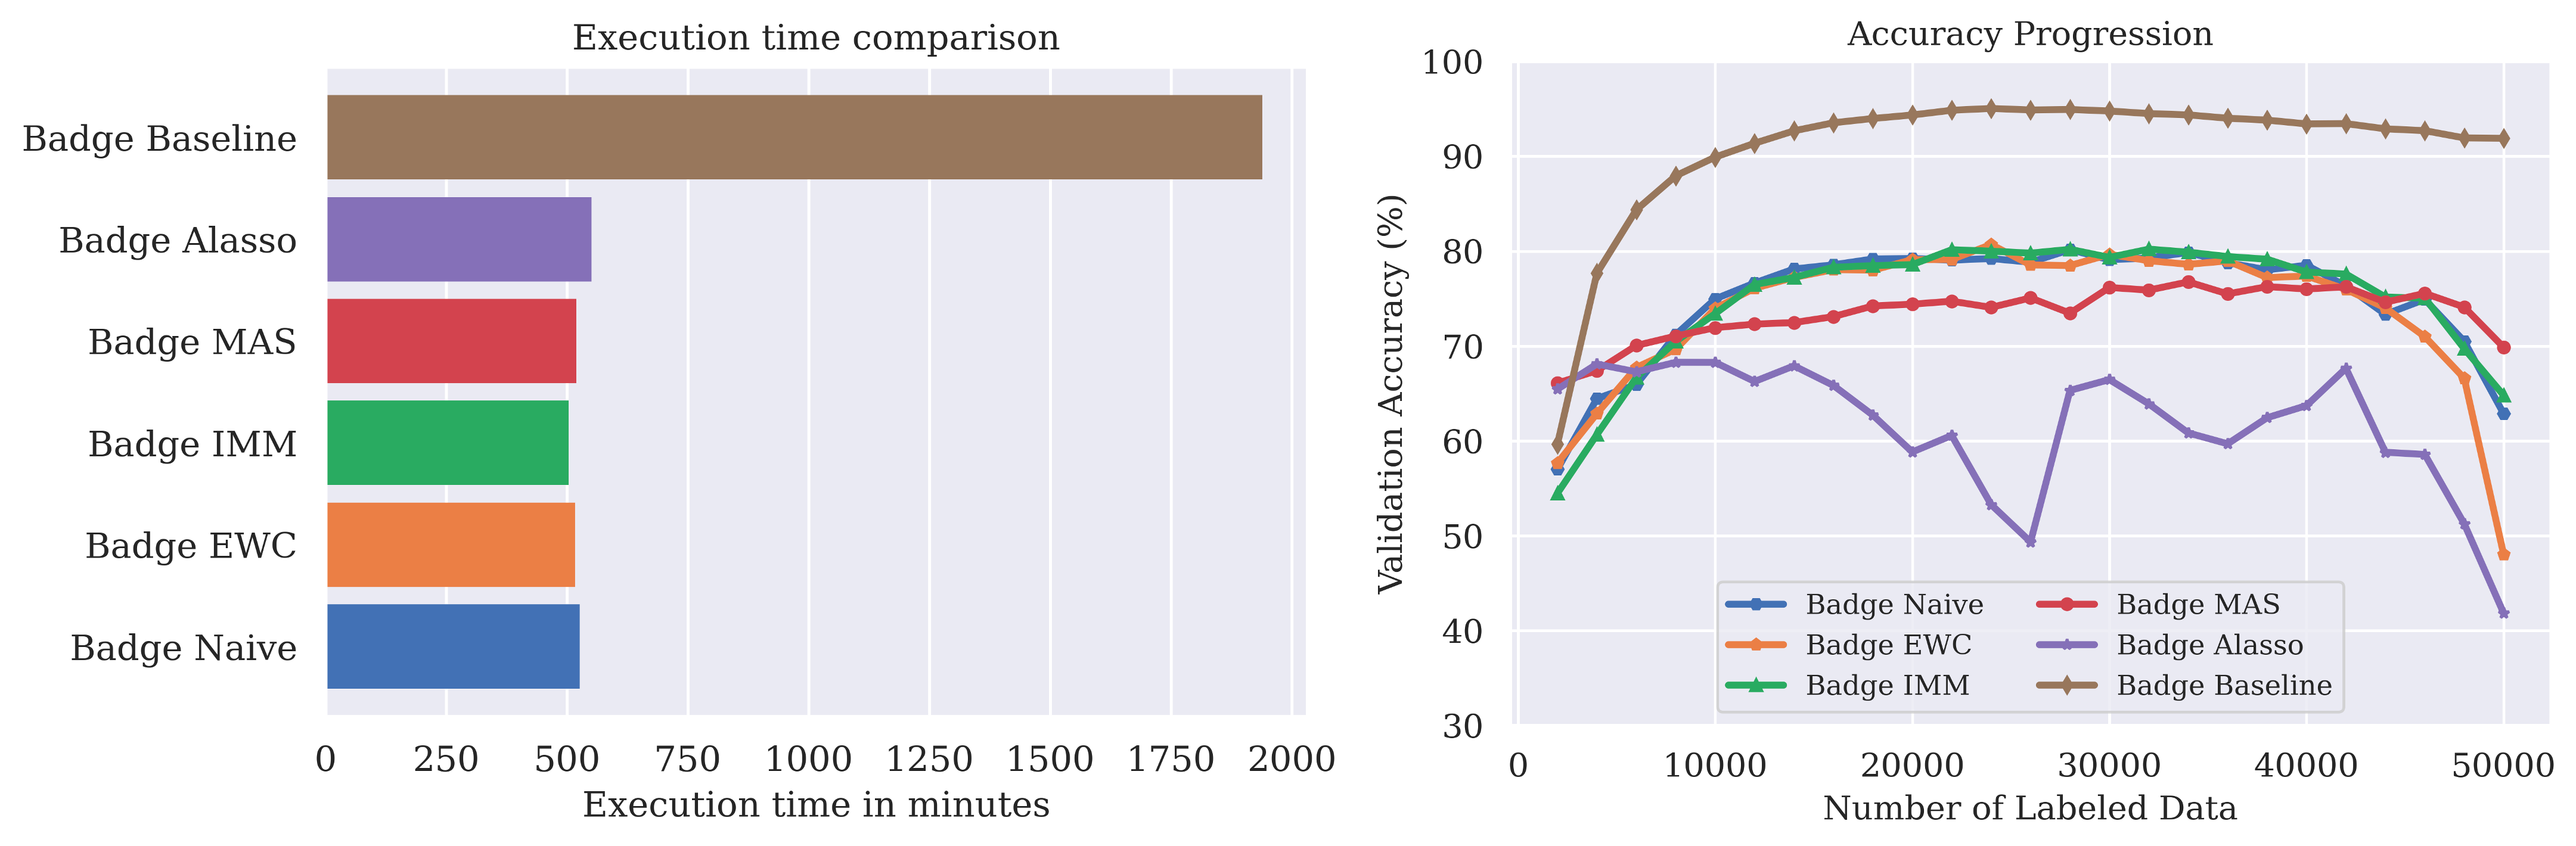
\includegraphics[width=\linewidth]{images/results_CAL/Badge_CAL_2000b.png}
    \caption[Continual Active Learning \gls{badge} 2000 batch size]{Comparison of execution time and validation accuracy of Continual Learning strategies used with the Active Learning strategy
    \gls{badge}. We use a batch size of 2000 for the experiments.}
    \label{fig:Evaluation:Results:CAL:Badge2000}
\end{figure}

Motivated by the increase in validation accuracy of the Continual Learning strategies with increasing batch size, we decide to re-run the experiments with a batch size of 4000. We start with the Active Learning
strategy Random. The results can be found in figure \ref{fig:Evaluation:Results:CAL:Random4000}. The gap in execution time between the baseline and the Continual Learning strategies has further decreased. \gls{imm} is
the fastest strategy, followed by \gls{mas}, \gls{ewc} and Naive who perform on the same level in terms of execution time. \gls{alasso} is the slowest strategy, but is still about 6 times as fast as the baseline. There is still a
gap in validation accuracy between the baseline and the Continual Learning strategies, however it is smaller than in the experiment with batch size 2000. Overall, \gls{ewc} and Naive perform best, followed by \gls{imm} and \gls{mas}.
\gls{alasso} starts of as the best strategy but suffers from a heavy decrease in validation accuracy, starting at around 8000 samples. \par

\begin{figure}[h]
    \centering
    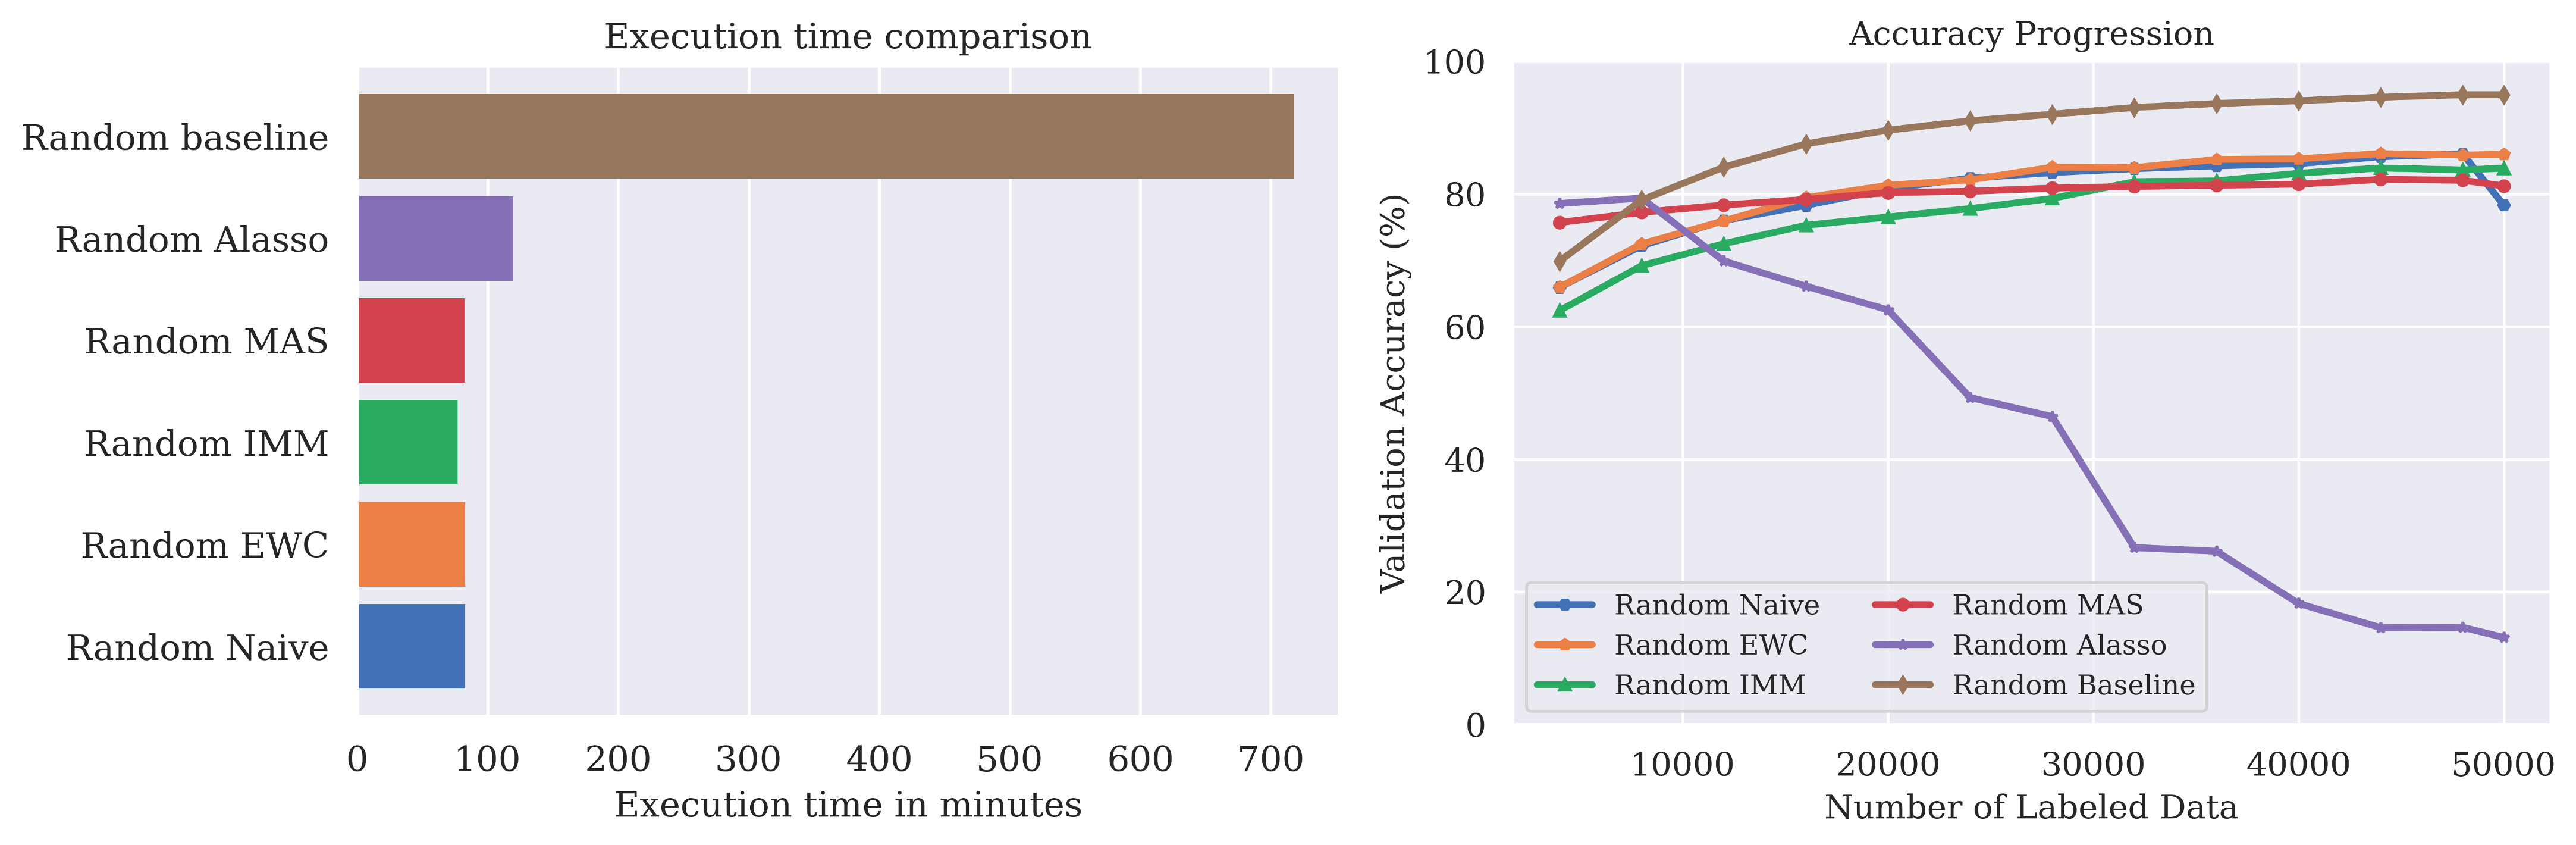
\includegraphics[width=\linewidth]{images/results_CAL/Random_CAL_4000b.png}
    \caption[Continual Active Learning Random 4000 batch size]{Comparison of execution time and validation accuracy of Continual Learning strategies used with the Active Learning strategy
    Random. We use a batch size of 4000 for the experiments}
    \label{fig:Evaluation:Results:CAL:Random4000}
\end{figure}

Next, we re-run the previous experiment with the Active Learning strategy \gls{lc}, again using a batch size of 4000. We present the results of the experiment in Figure \ref{fig:Evaluation:Results:CAL:LC4000}. In terms of runtime,
the results are similar to the experiment with Random, with \gls{alasso} being the slowest Continual Learning strategy, followed by \gls{mas}, \gls{ewc}, \gls{imm} and Naive. All Continual Learning strategies are significantly faster than the baseline,
with \gls{alasso} being about 6 times as fast and Naive about 10 times as fast. The gap in validation accuracy between the baseline and the Continual Learning strategies remains significant, although it has shrunk compared to the
experiment with 2000 batch size. \gls{imm}, \gls{ewc} and Naive perform almost identically across the experiment with \gls{mas} following closely and outperforming the remaining strategies within the last 5000 samples. \gls{alasso} starts of on par
with the remaining strategies, but suffers from a heavy decrease in validation accuracy at around 8000 samples. \par

\begin{figure}[h]
    \centering
    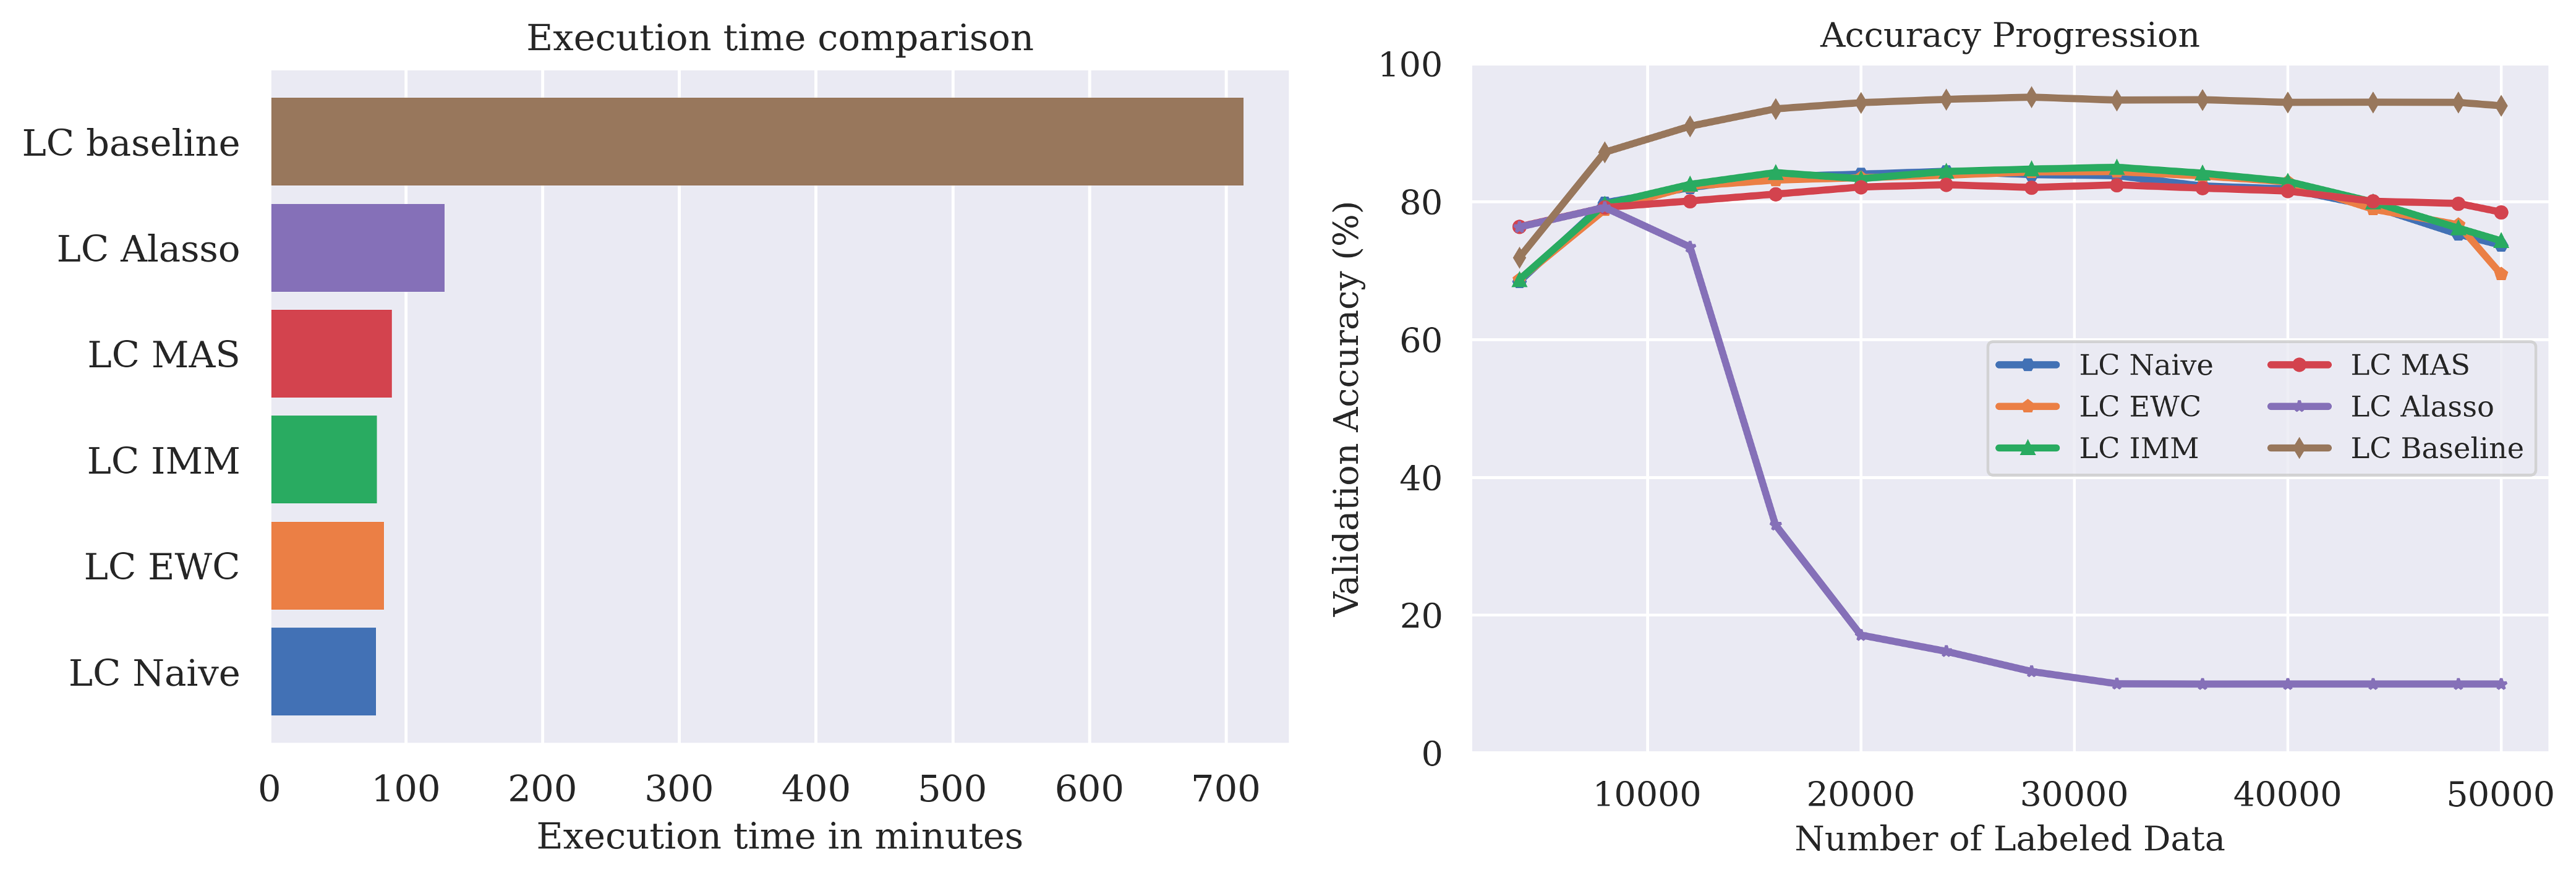
\includegraphics[width=\linewidth]{images/results_CAL/LC_CAL_4000b.png}
    \caption[Continual Active Learning \gls{lc} 4000 batch size]{Comparison of execution time and validation accuracy of Continual Learning strategies used with the Active Learning strategy
    \gls{lc}. We use a batch size of 4000 for the experiments. }
    \label{fig:Evaluation:Results:CAL:LC4000}
\end{figure}

The third experiment with a batch size of 4000 is run with the Active Learning strategy \gls{bald}. The results of the experiment can be found in figure \ref{fig:Evaluation:Results:CAL:BALD4000}. The ranking of execution time of the Continual
Learning strategies and the baseline is similar to the previous experiment with \gls{lc}. In terms of accuracy, there remains a large gap between the baseline and all Continual Learning strategies. Naive, \gls{imm} and \gls{ewc} perform similar, showing an
s-shaped validation accuracy curve. The performance of \gls{mas} follows a similar curve, however \gls{mas} performs better in the first half of the experiment, and worse in the second half compared to the three former strategies. \gls{alasso} starts off as
the best Continual Learning strategy, but its validation accuracy decreases steadily over the course of the experiment, until it suffers a huge drop in the final iteration. \par 

\begin{figure}[h]
    \centering
    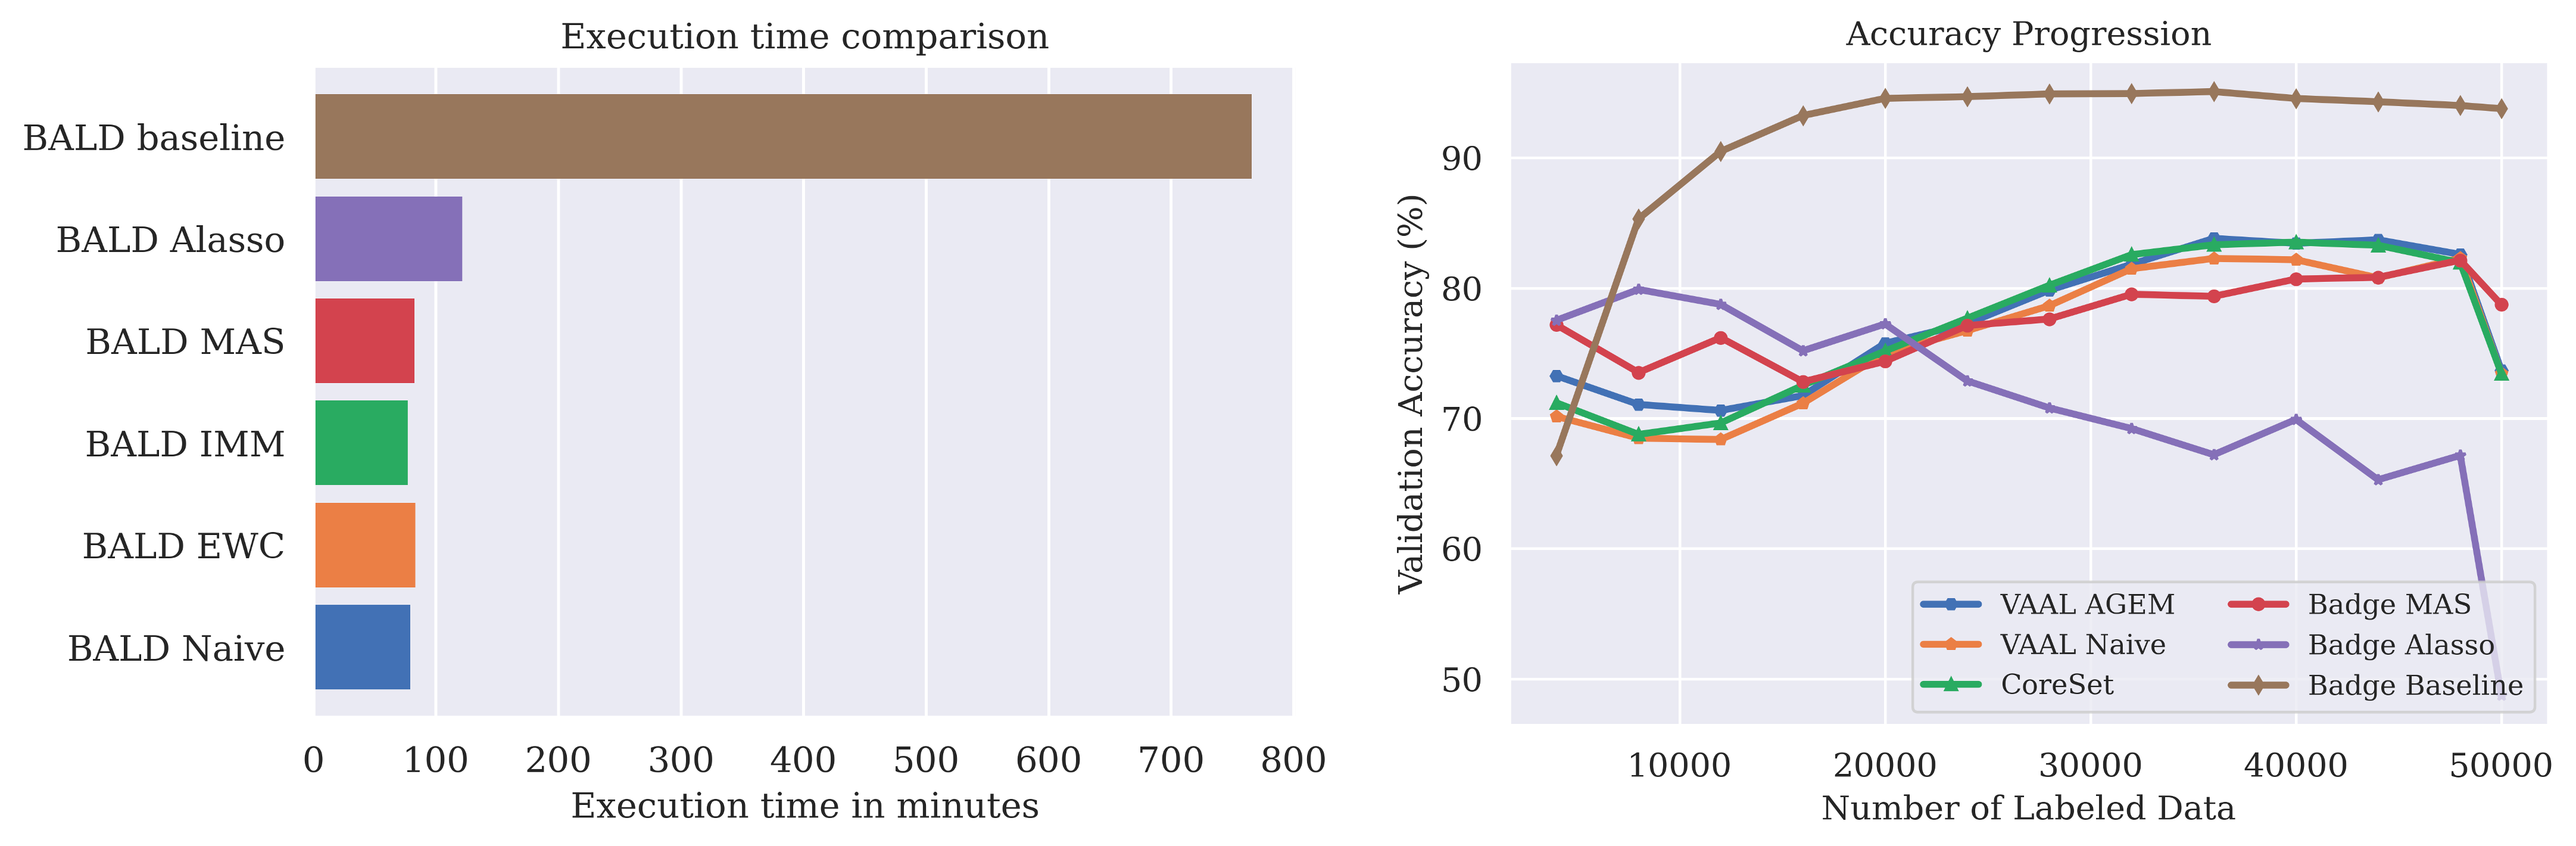
\includegraphics[width=\linewidth]{images/results_CAL/Bald_CAL_4000b.png}
    \caption[Continual Active Learning \gls{bald} 4000 batch size]{Comparison of execution time and validation accuracy of Continual Learning strategies used with the Active Learning strategy
    \gls{bald}. We use a batch size of 4000 for the experiments }
    \label{fig:Evaluation:Results:CAL:BALD4000}
\end{figure}


We now run the experiment with the identical setup with the Active Learning strategy CoreSet. Our results are presented in figure \ref{fig:Evaluation:Results:CAL:CoreSet4000}. The gap in execution time between the baseline and the Continual Learning 
strategies has further decreased. \gls{imm} is the fastest Continual Learning strategy, being about 6 times as fast as the baseline. On the other hand, \gls{alasso} is the slowest Continual Learning strategy, boasting around one fourth of the execution time of the
baseline. Not only the gap in execution time has decreased compared to the experiment with batch size 2000, but also the gap in validation accuracy. Naive is the best performing strategy, lacking only 10 percentage points in validation accuracy to the
baseline during the first half of the experiment. \gls{imm}, \gls{ewc} and \gls{mas} follow in that order, showing a similar validation accuracy curve as Naive. \gls{alasso} starts with a similar validation accuracy as the other Continual Learning strategies, but falls behind
after 8000 samples. \par


\begin{figure}[h]
    \centering
    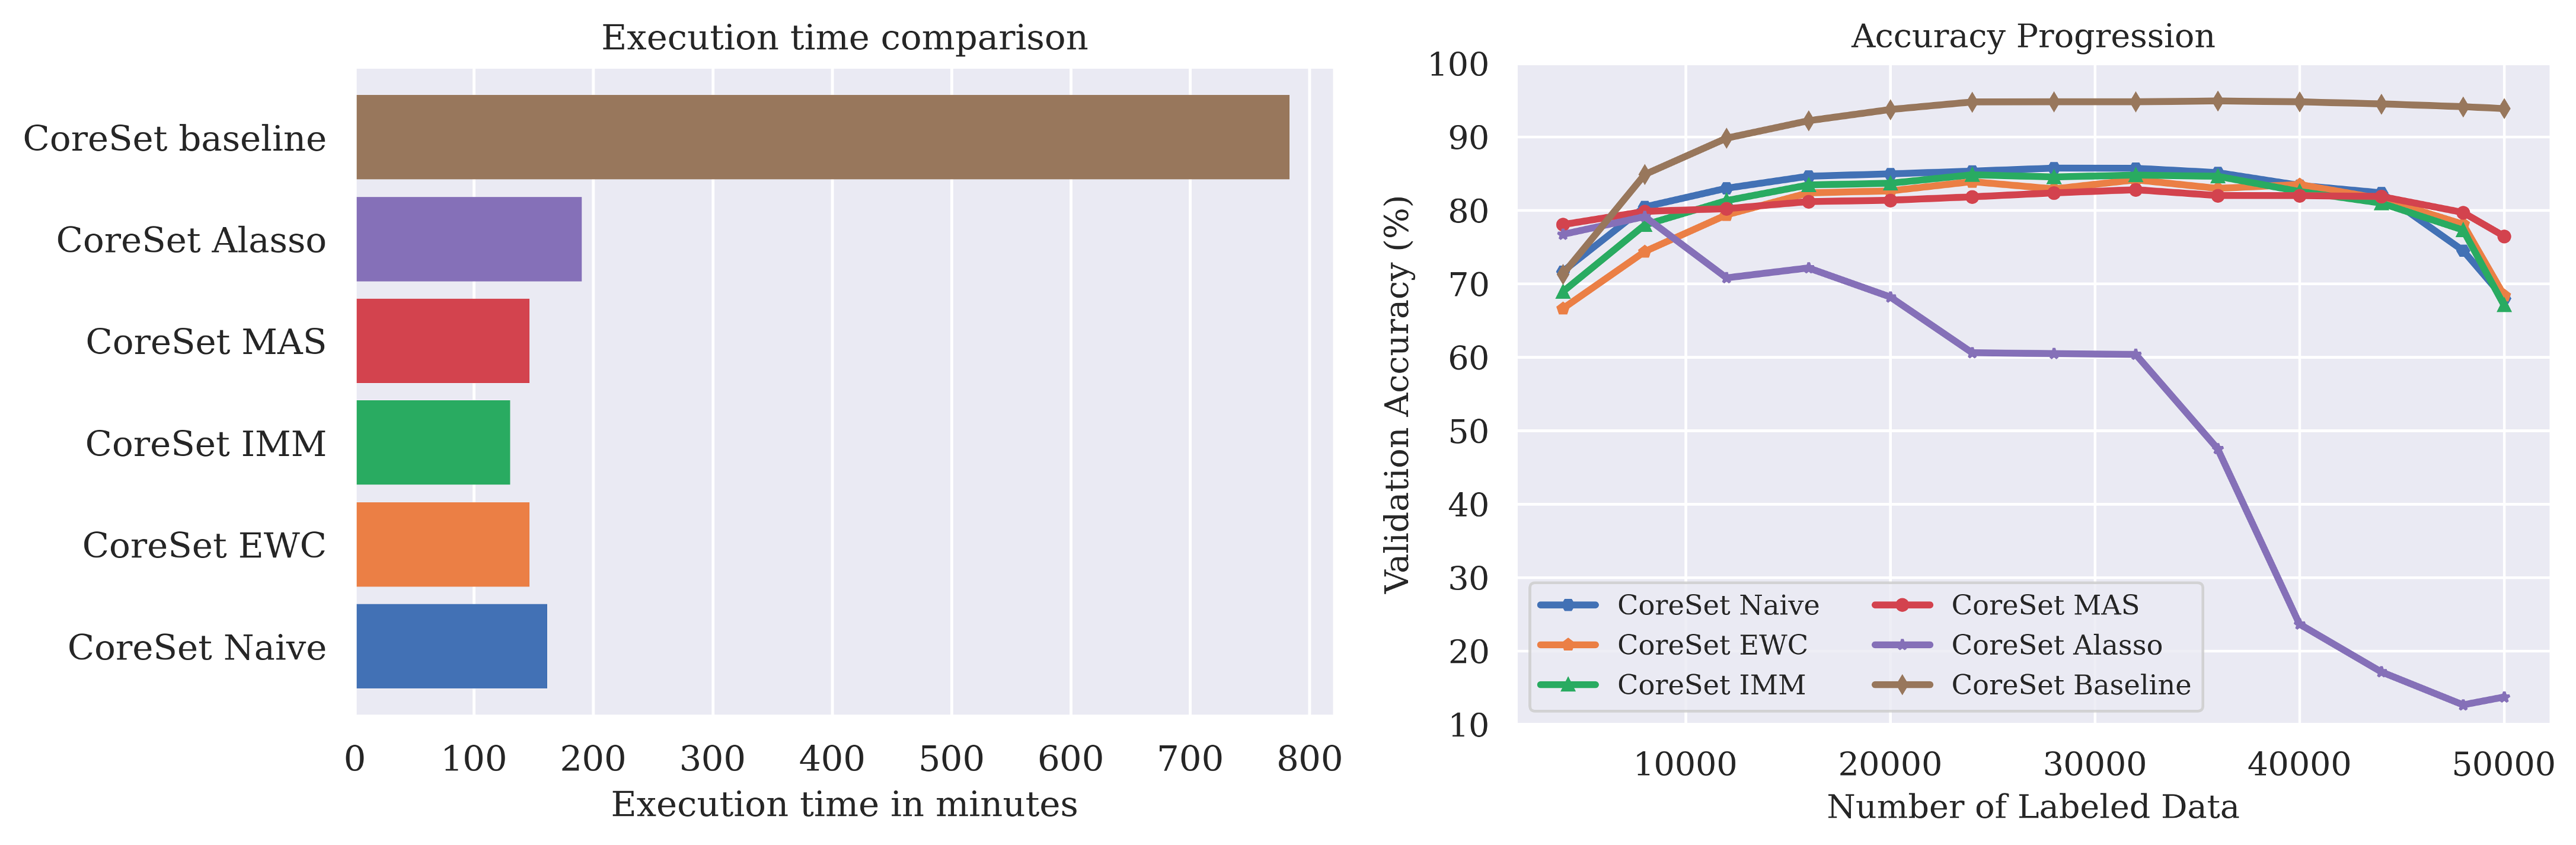
\includegraphics[width=\linewidth]{images/results_CAL/CoreSet_CAL_4000b.png}
    \caption[Continual Active Learning CoreSet 4000 batch size]{Comparison of execution time and validation accuracy of Continual Learning strategies used with the Active Learning strategy
    CoreSet. We use a batch size of 4000 for the experiments.}
    \label{fig:Evaluation:Results:CAL:CoreSet4000}
\end{figure}

Our final experiment with a batch size of 4000 is run with the Active Learning strategy \gls{badge}. The results of the experiment can be found in figure \ref{fig:Evaluation:Results:CAL:Badge4000}. Out of all experiments in this series, this one shows the
smallest gap in execution time between the baseline and the Continual Learning strategies. However, the baseline is still about 800 Minutes or 13 hours slower than all Continual Learning strategies. Just as in the experiment with 2000 batch size, the
execution time of the Contiual Learning strategies is comparable, with \gls{alasso} being the slowest and \gls{imm} being the fastest. Compared to the experiment with batch size 2000, the validation accuracy curve of all Continual Learning strategies has become smoother 
and the gap between the baseline and the Continual Learning strategies has decreased. The only exception to this is \gls{alasso}, which has a negative slope in its validation accuracy curve in the first half of the experiment, followed by a slight increase in 
validation accuracy and a huge drop in the end. \gls{imm}, \gls{ewc} and Naive perform similar for the first 45000 samples, where \gls{imm} falls behind the other two strategies. The validation accuracy of \gls{mas} is almost consistent throughout the experiment, with a slight
increase in the first half and a slight decrease in the second half. \par

\begin{figure}[h]
    \centering
    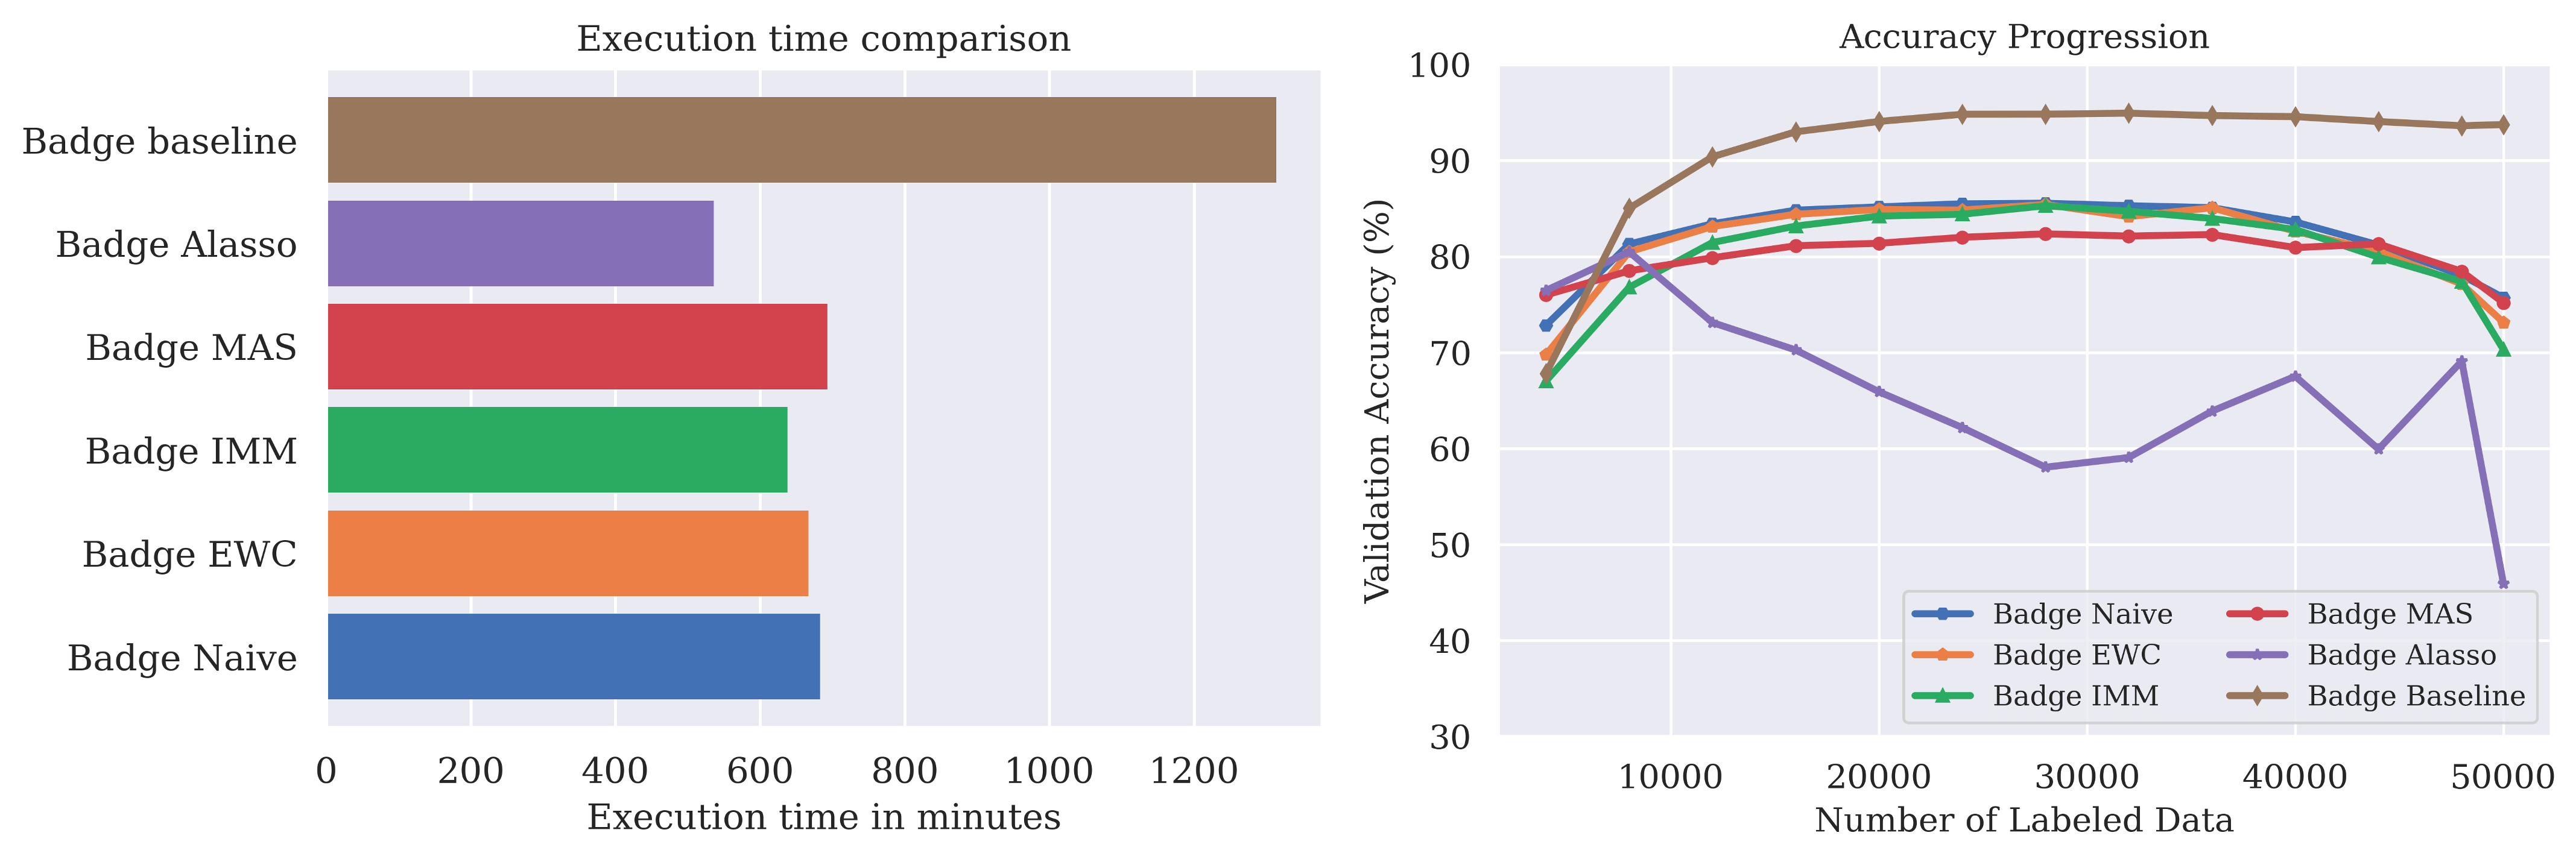
\includegraphics[width=\linewidth]{images/results_CAL/Badge_CAL_4000b.png}
    \caption[Continual Active Learning \gls{badge} 4000 batch size]{Comparison of execution time and validation accuracy of Continual Learning strategies used with the Active Learning strategy
    \gls{badge}. We use a batch size of 4000 for the experiments.}
    \label{fig:Evaluation:Results:CAL:Badge4000}
\end{figure}

%Test of multiple images in a figure
\begin{figure}[h]
    \centering
    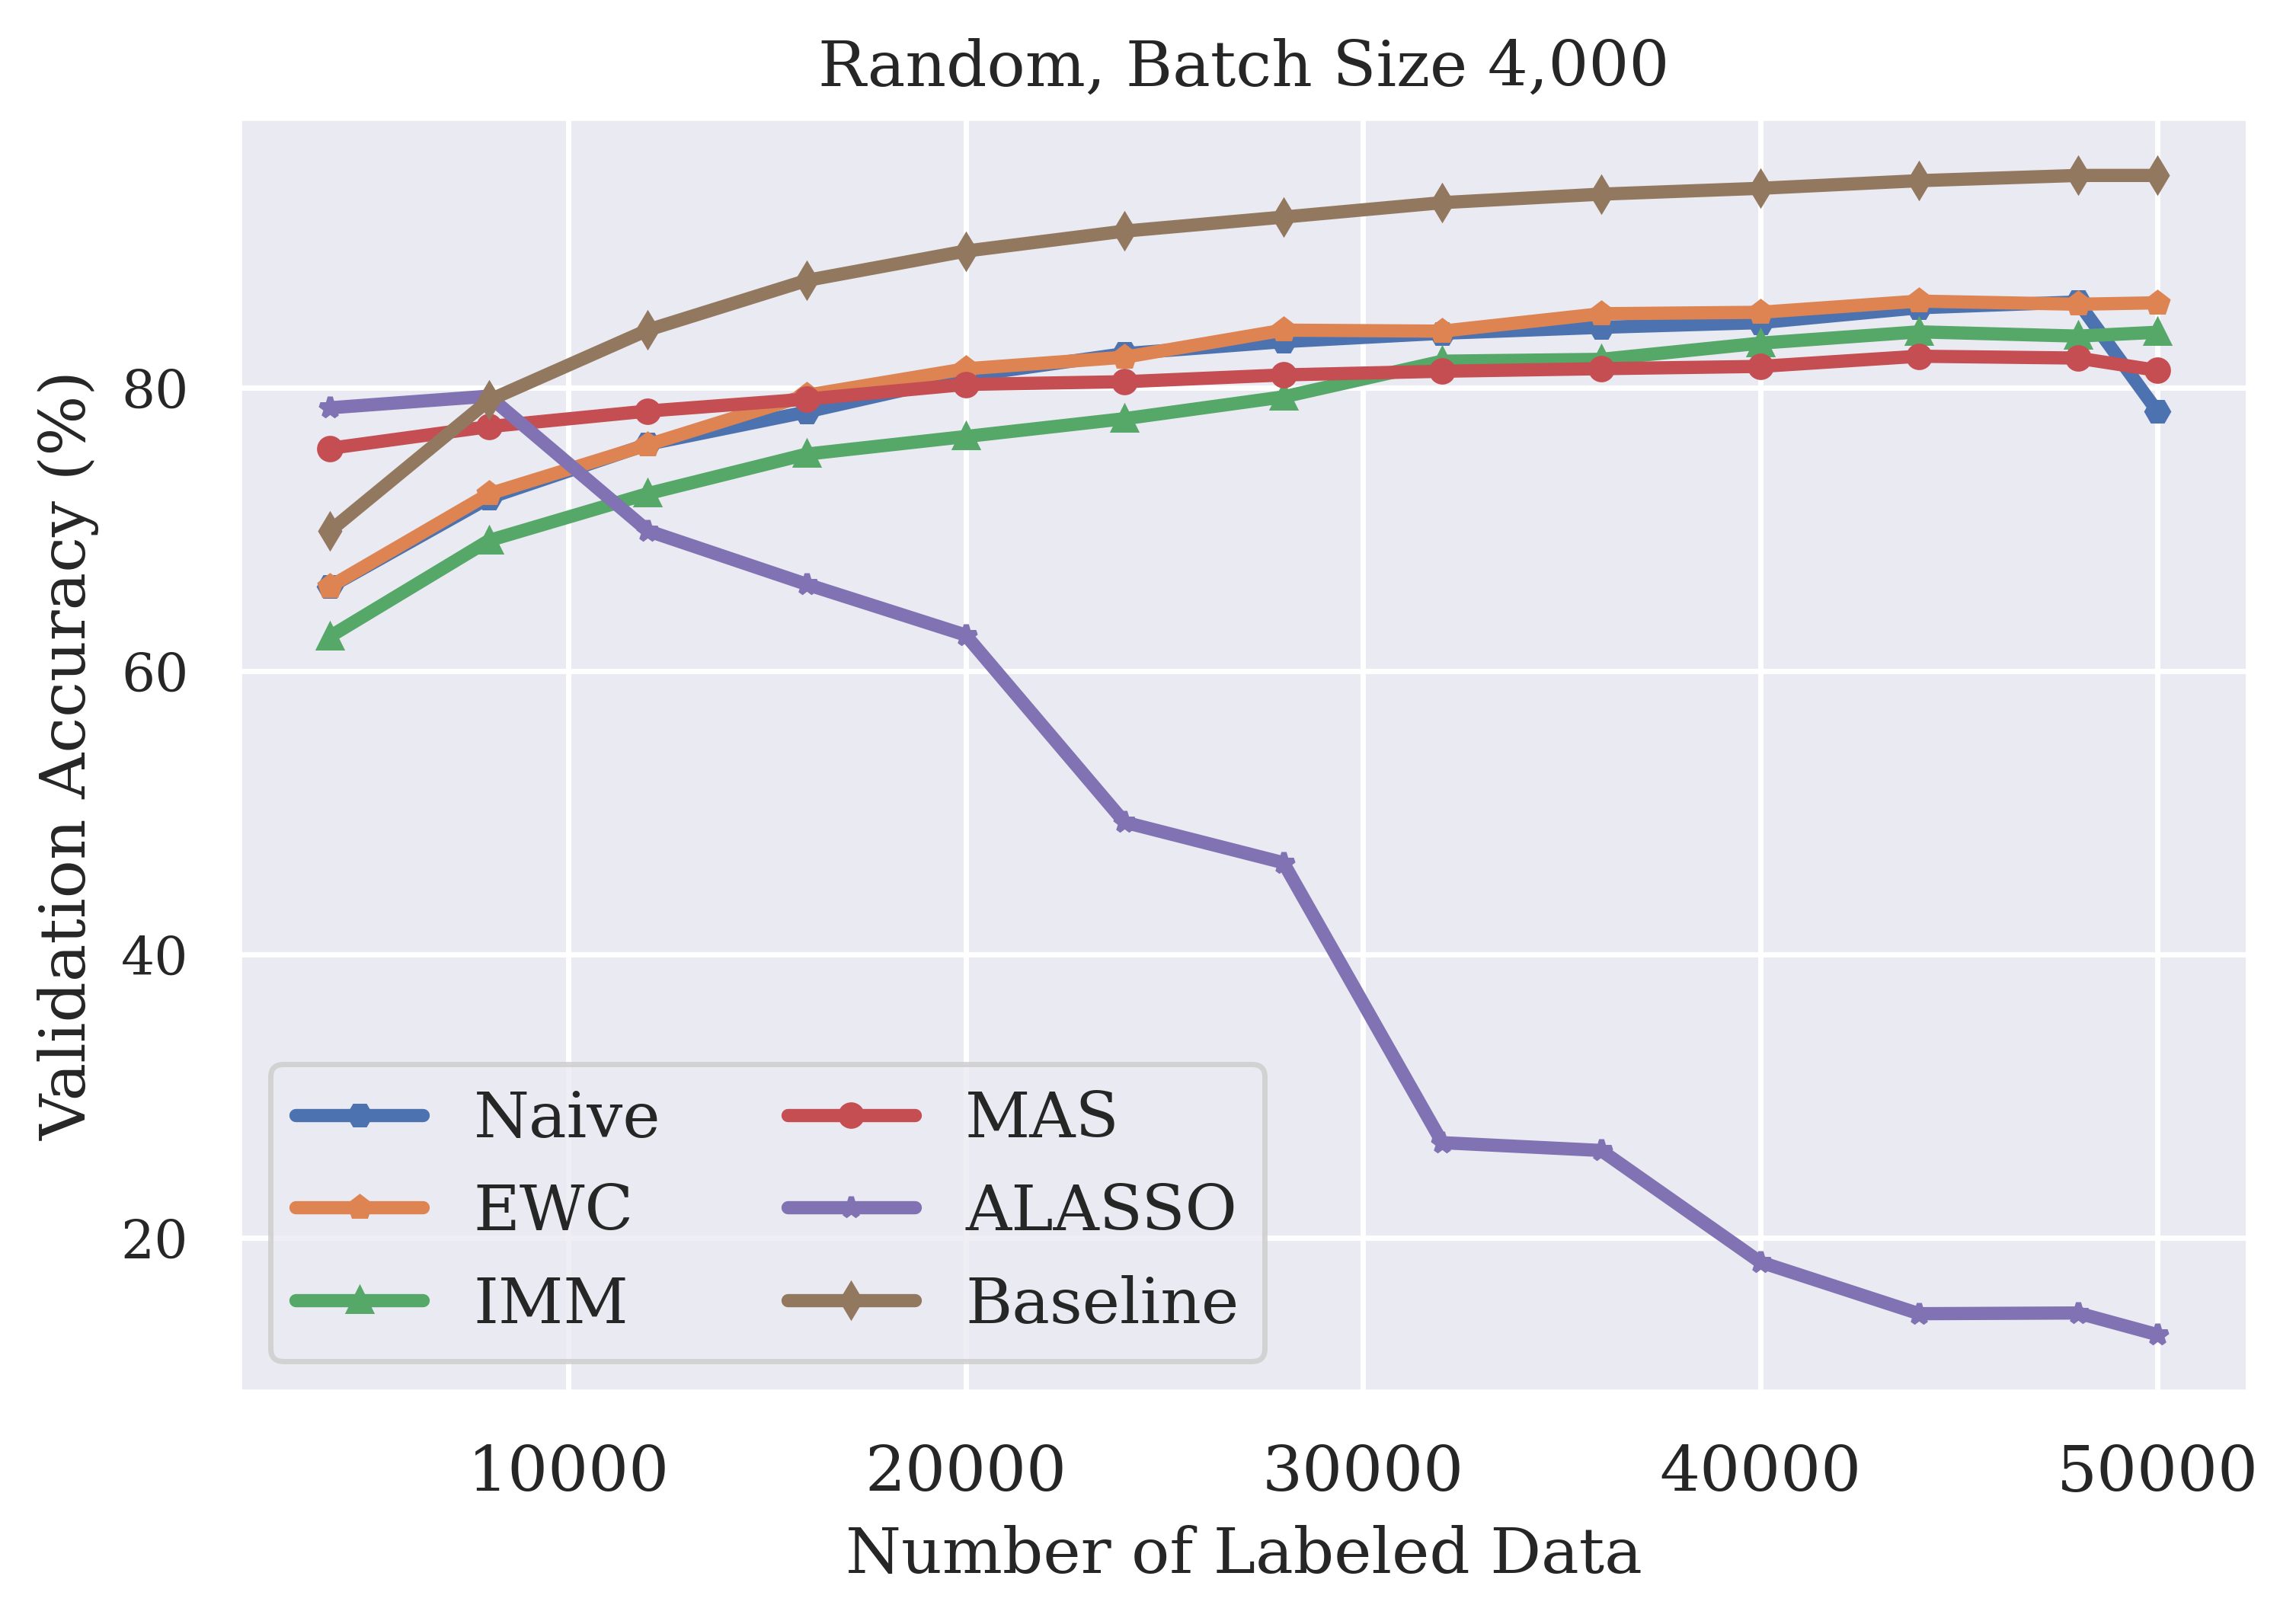
\includegraphics[width=0.3\linewidth]{images/results_CAL/random_4000b_acc.png} \hfill
    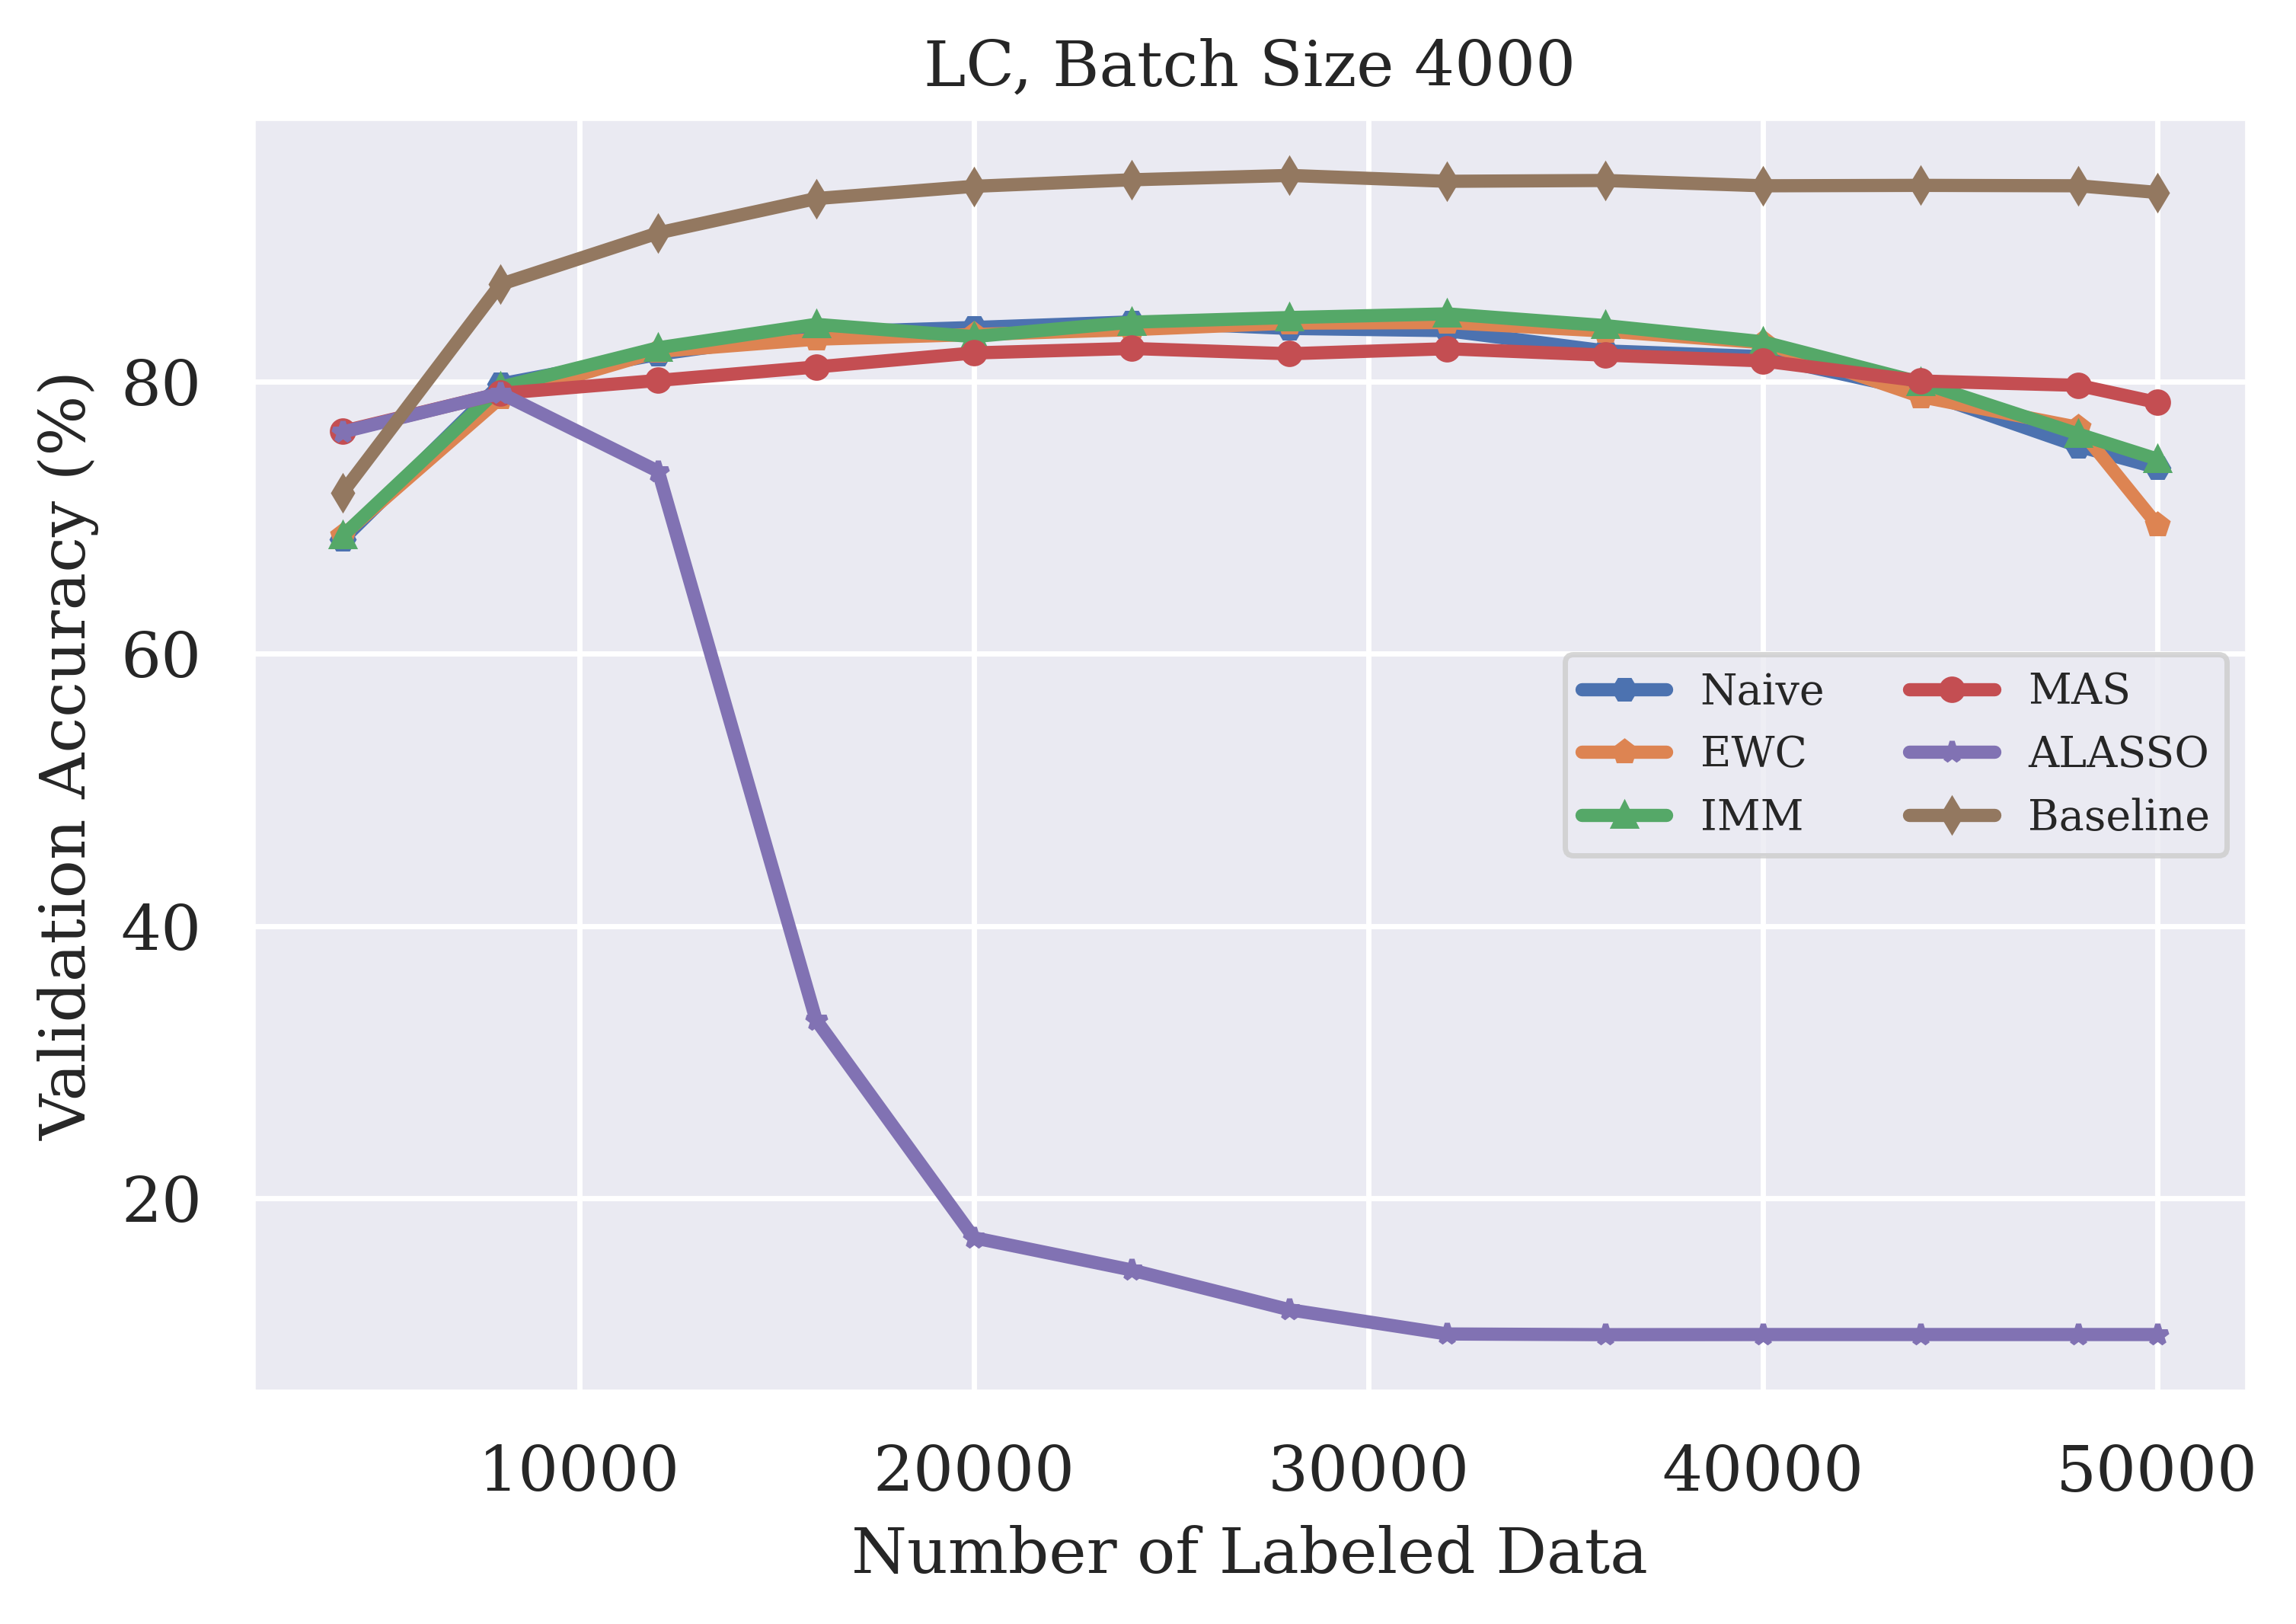
\includegraphics[width=0.3\linewidth]{images/results_CAL/lc_4000b_acc.png} \hfill
    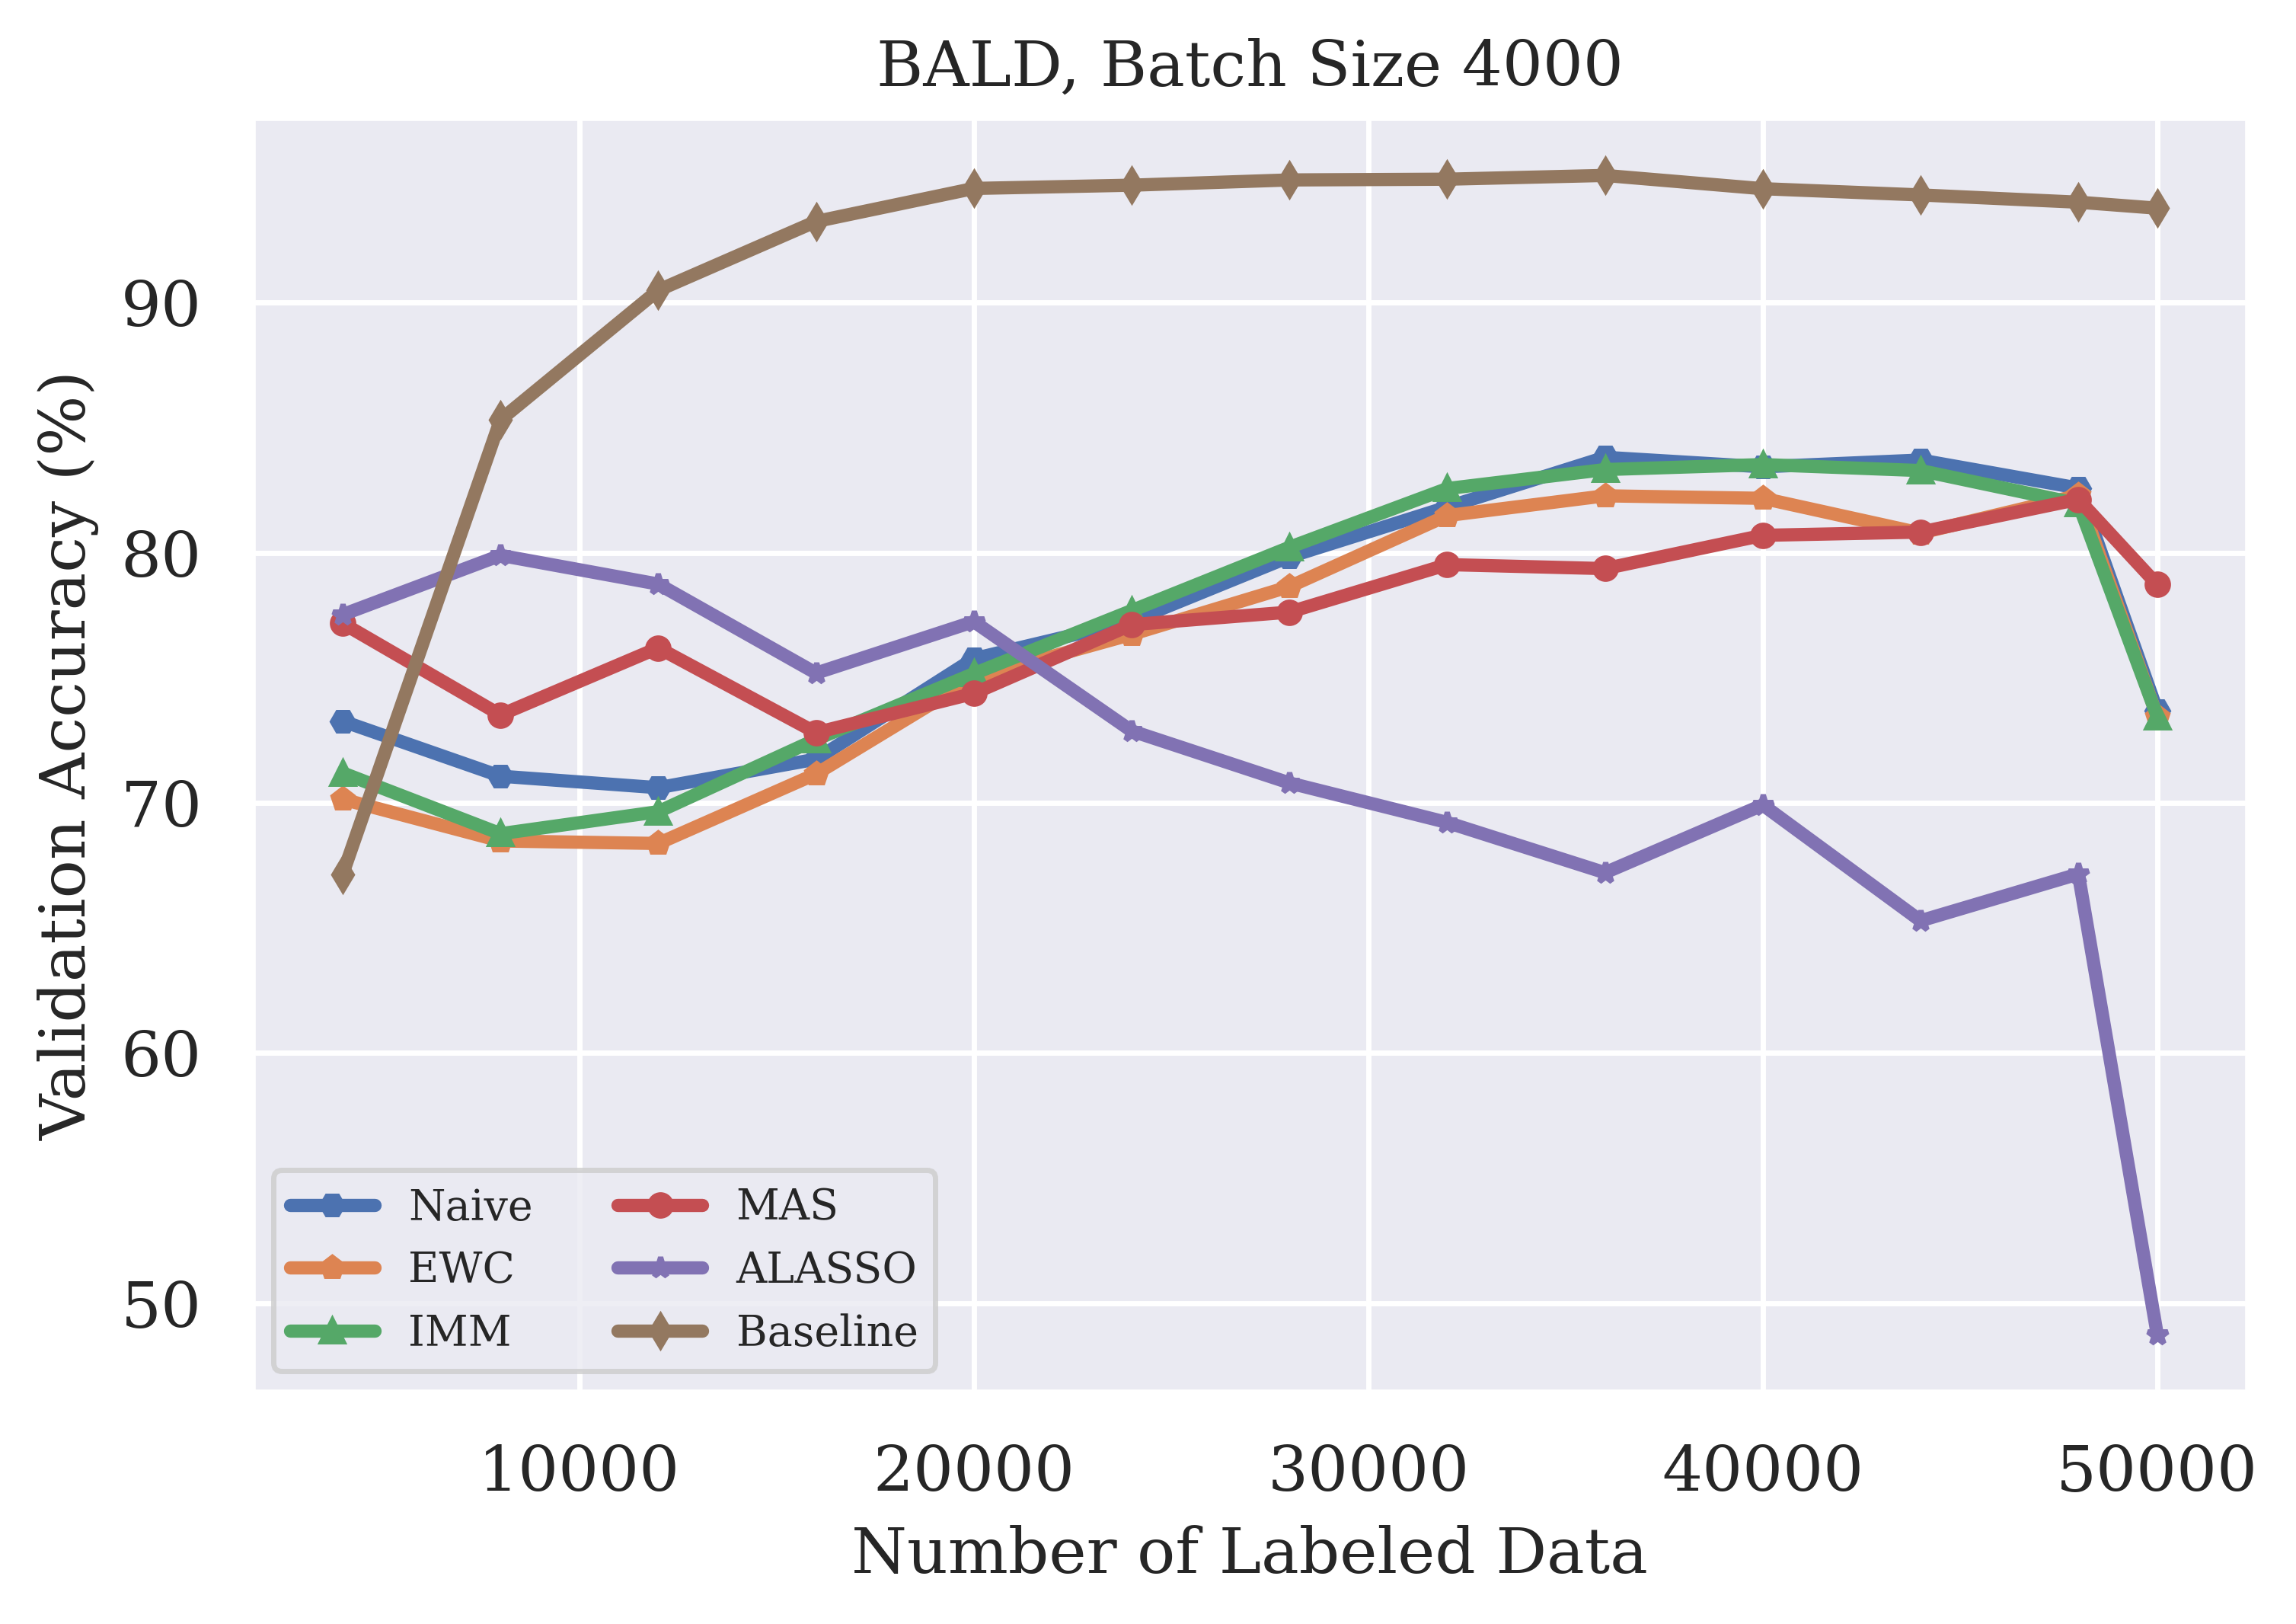
\includegraphics[width=0.3\linewidth]{images/results_CAL/bald_4000b_acc.png}
    \\[\smallskipamount]
    \hfill 
    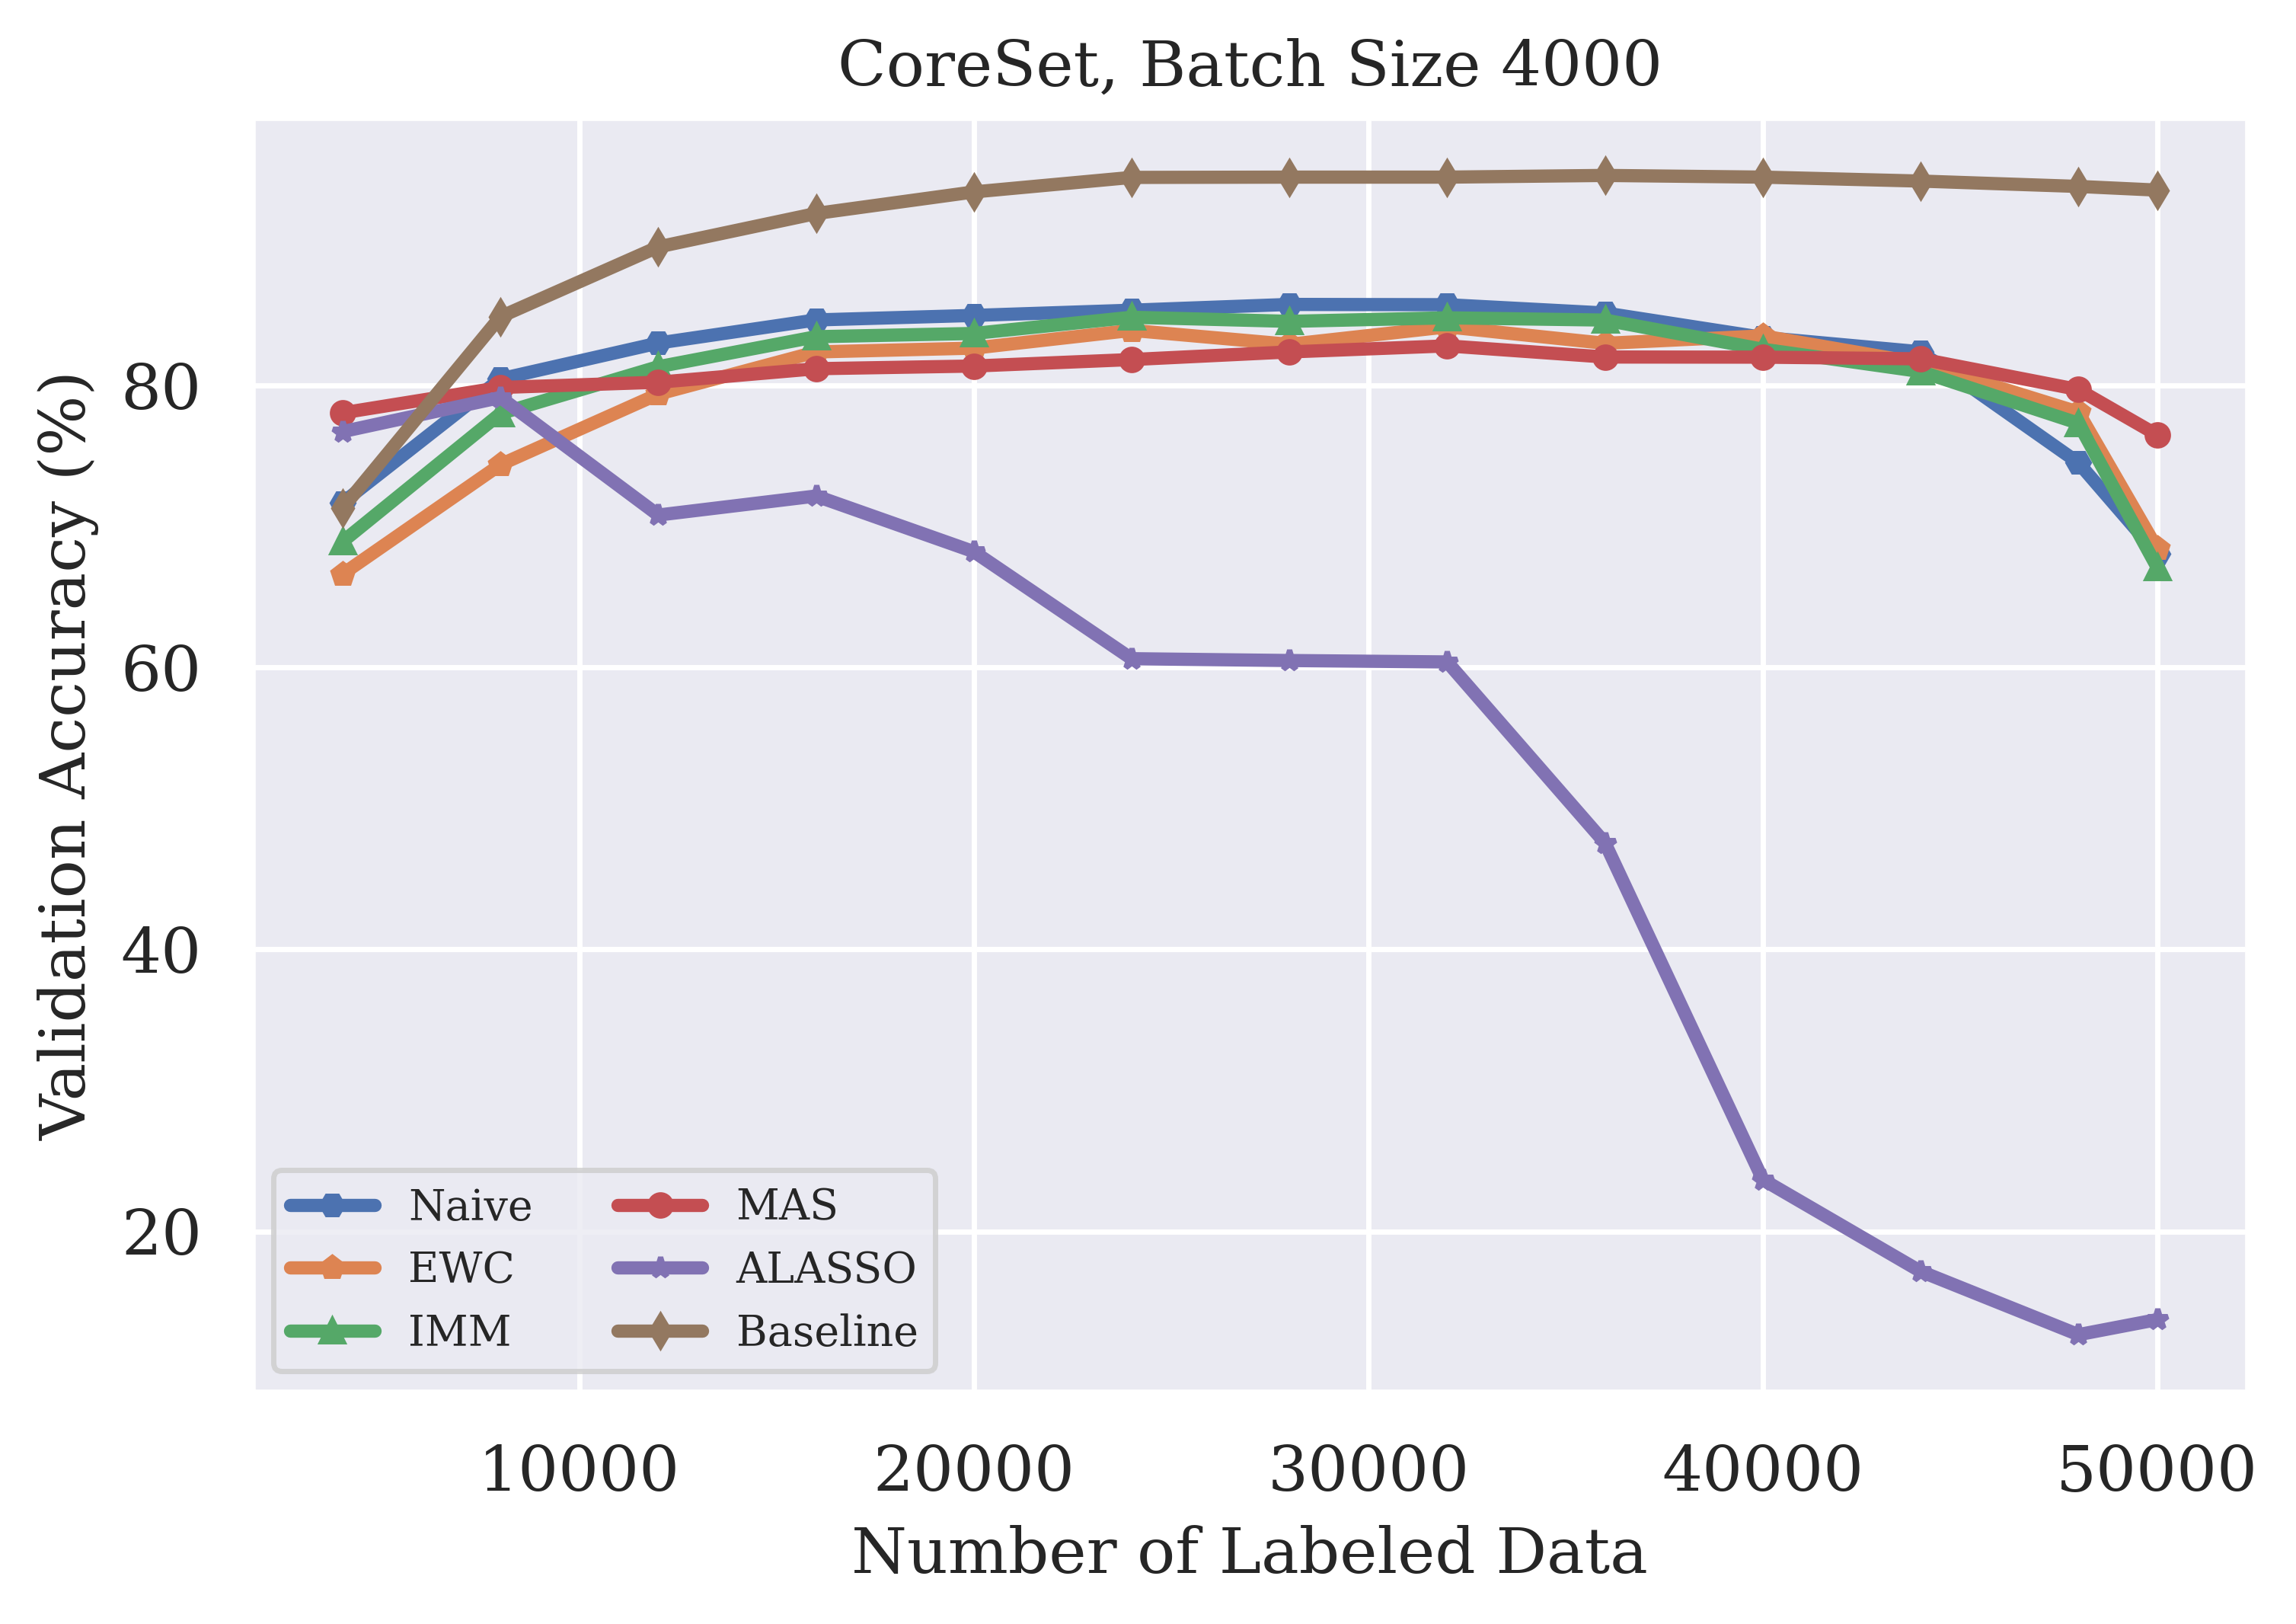
\includegraphics[width=0.3\linewidth]{images/results_CAL/coreset_4000b_acc.png} \hfill
    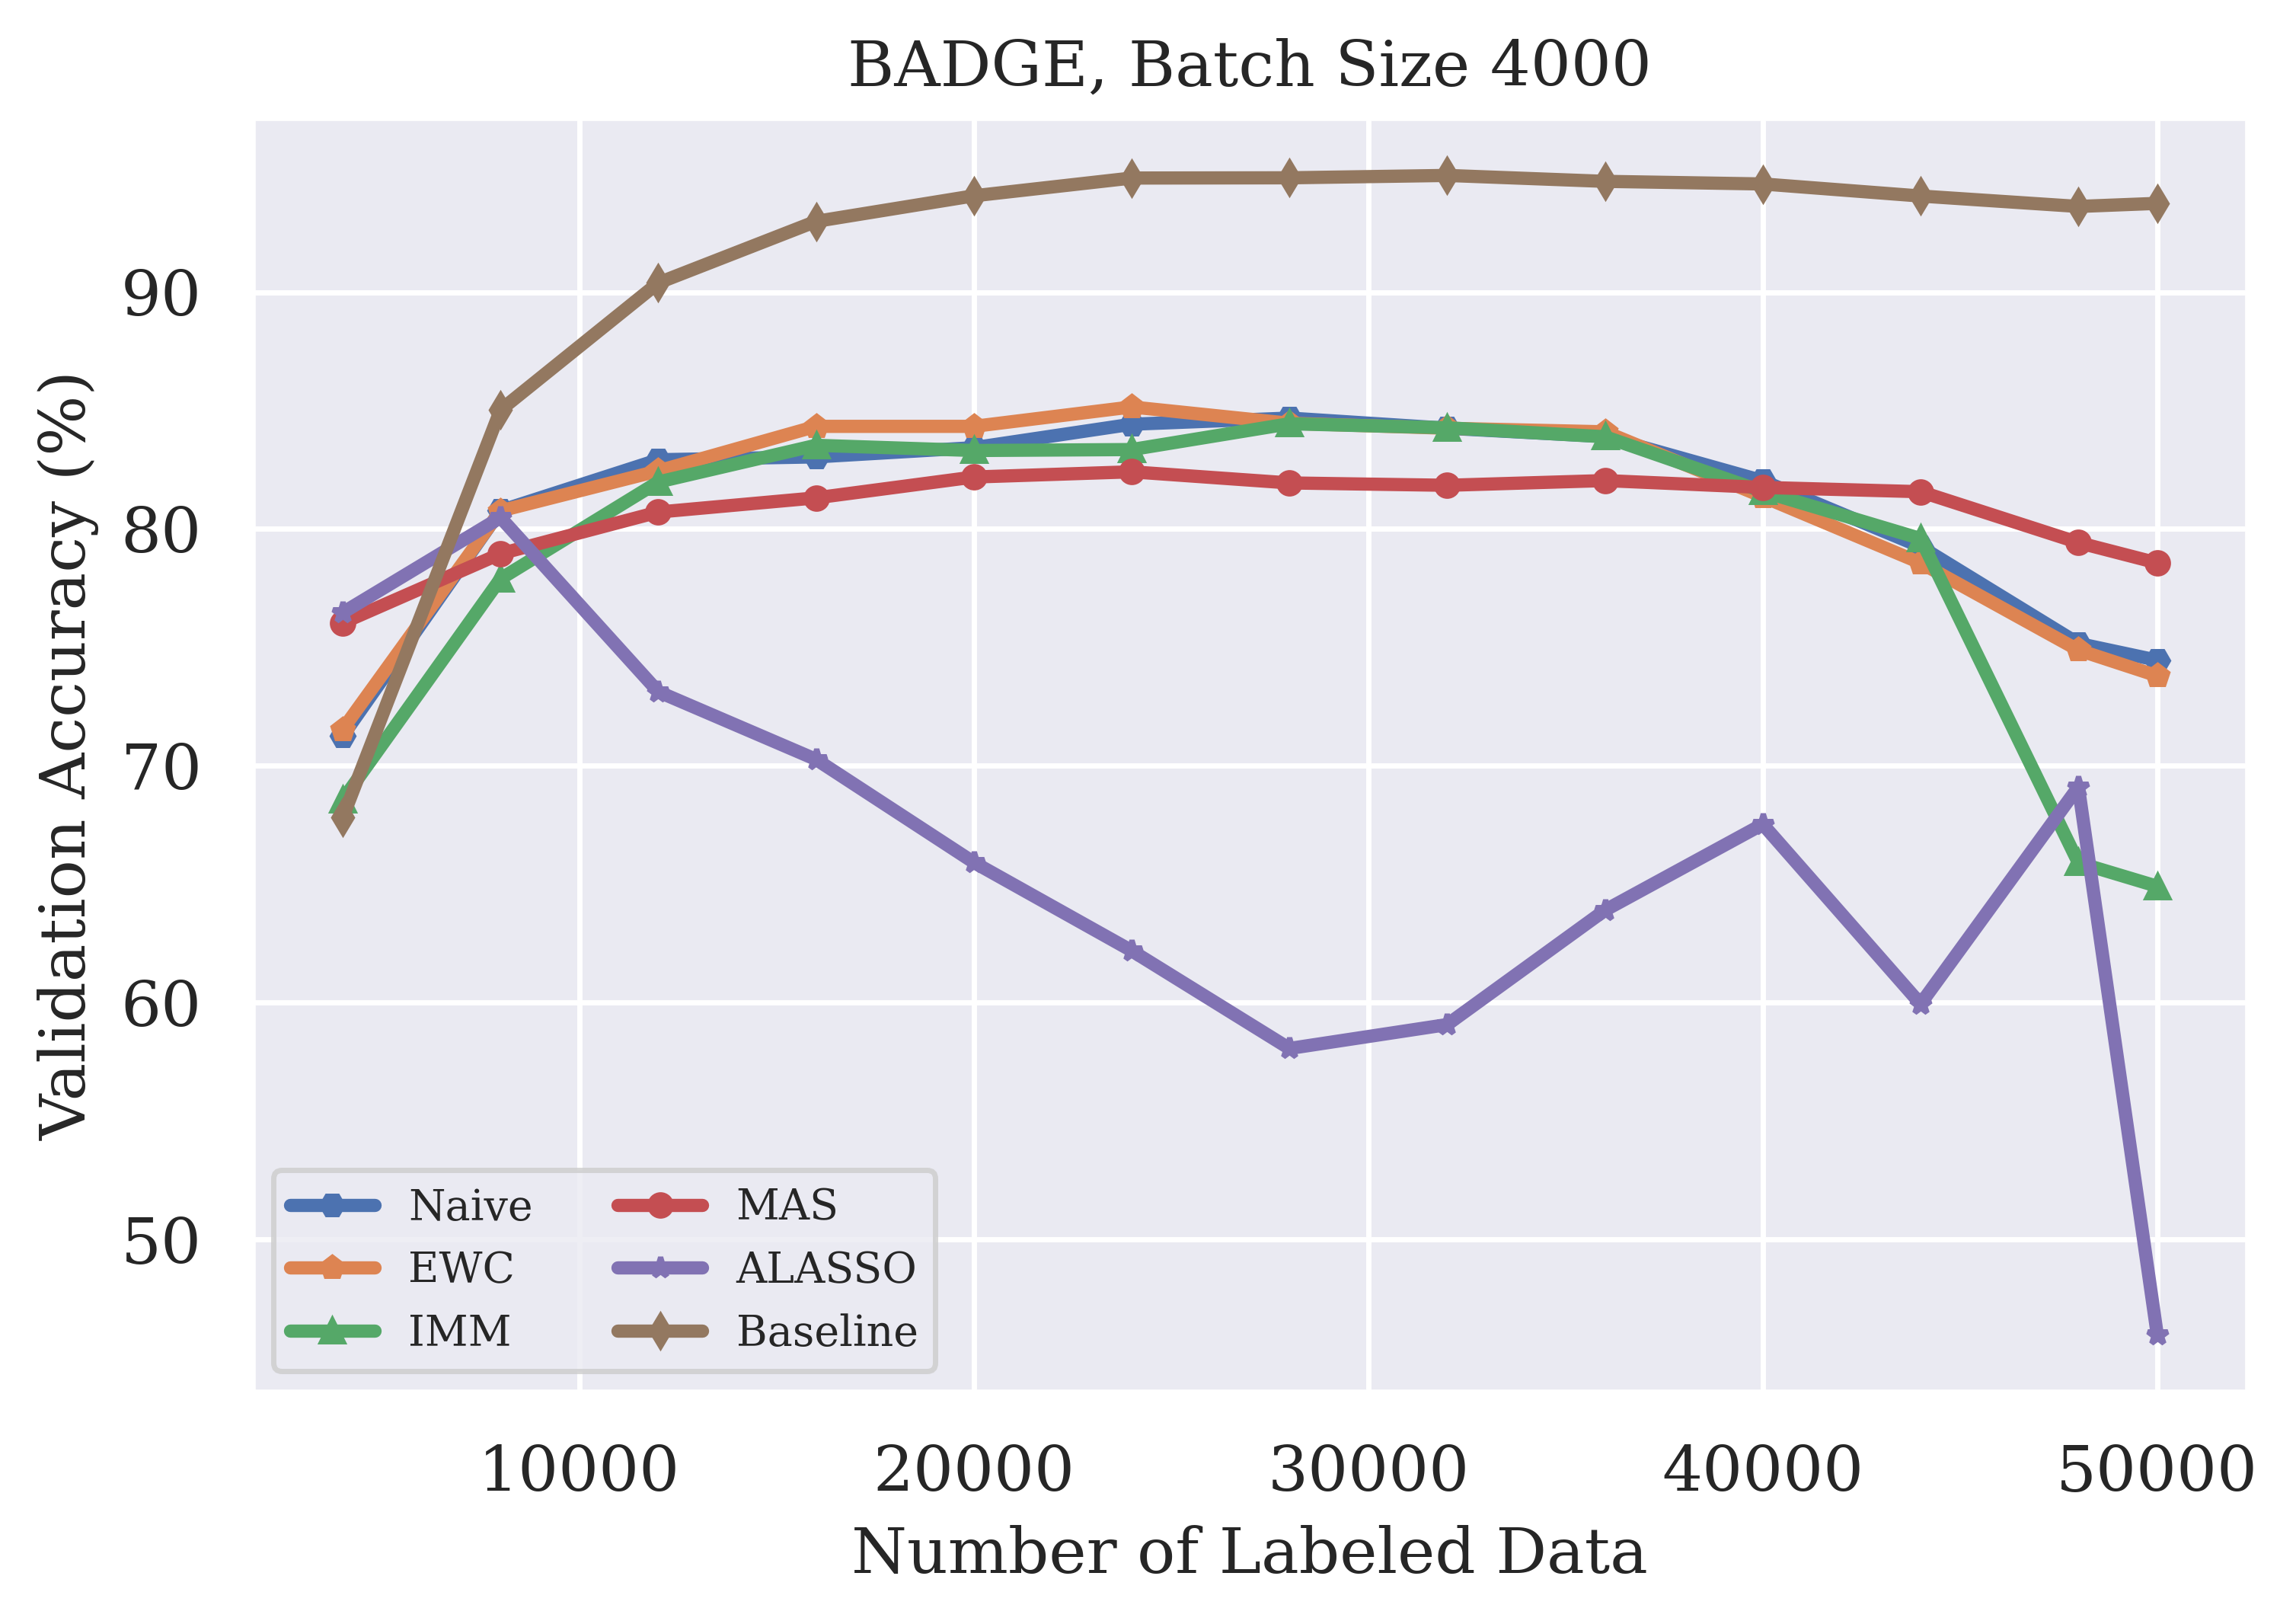
\includegraphics[width=0.3\linewidth]{images/results_CAL/badge_4000b_acc.png} \hfill
    \caption[Continual Active Learning with \gls{badge} with varying batch size]{Comparison of validation accuracy of Continual Learning and Active Learning strategies
    with batch size 4000.}
    \label{fig:Evaluation:Results:CAL:4000bAcc}
\end{figure}

\begin{figure}[h]
    \centering
    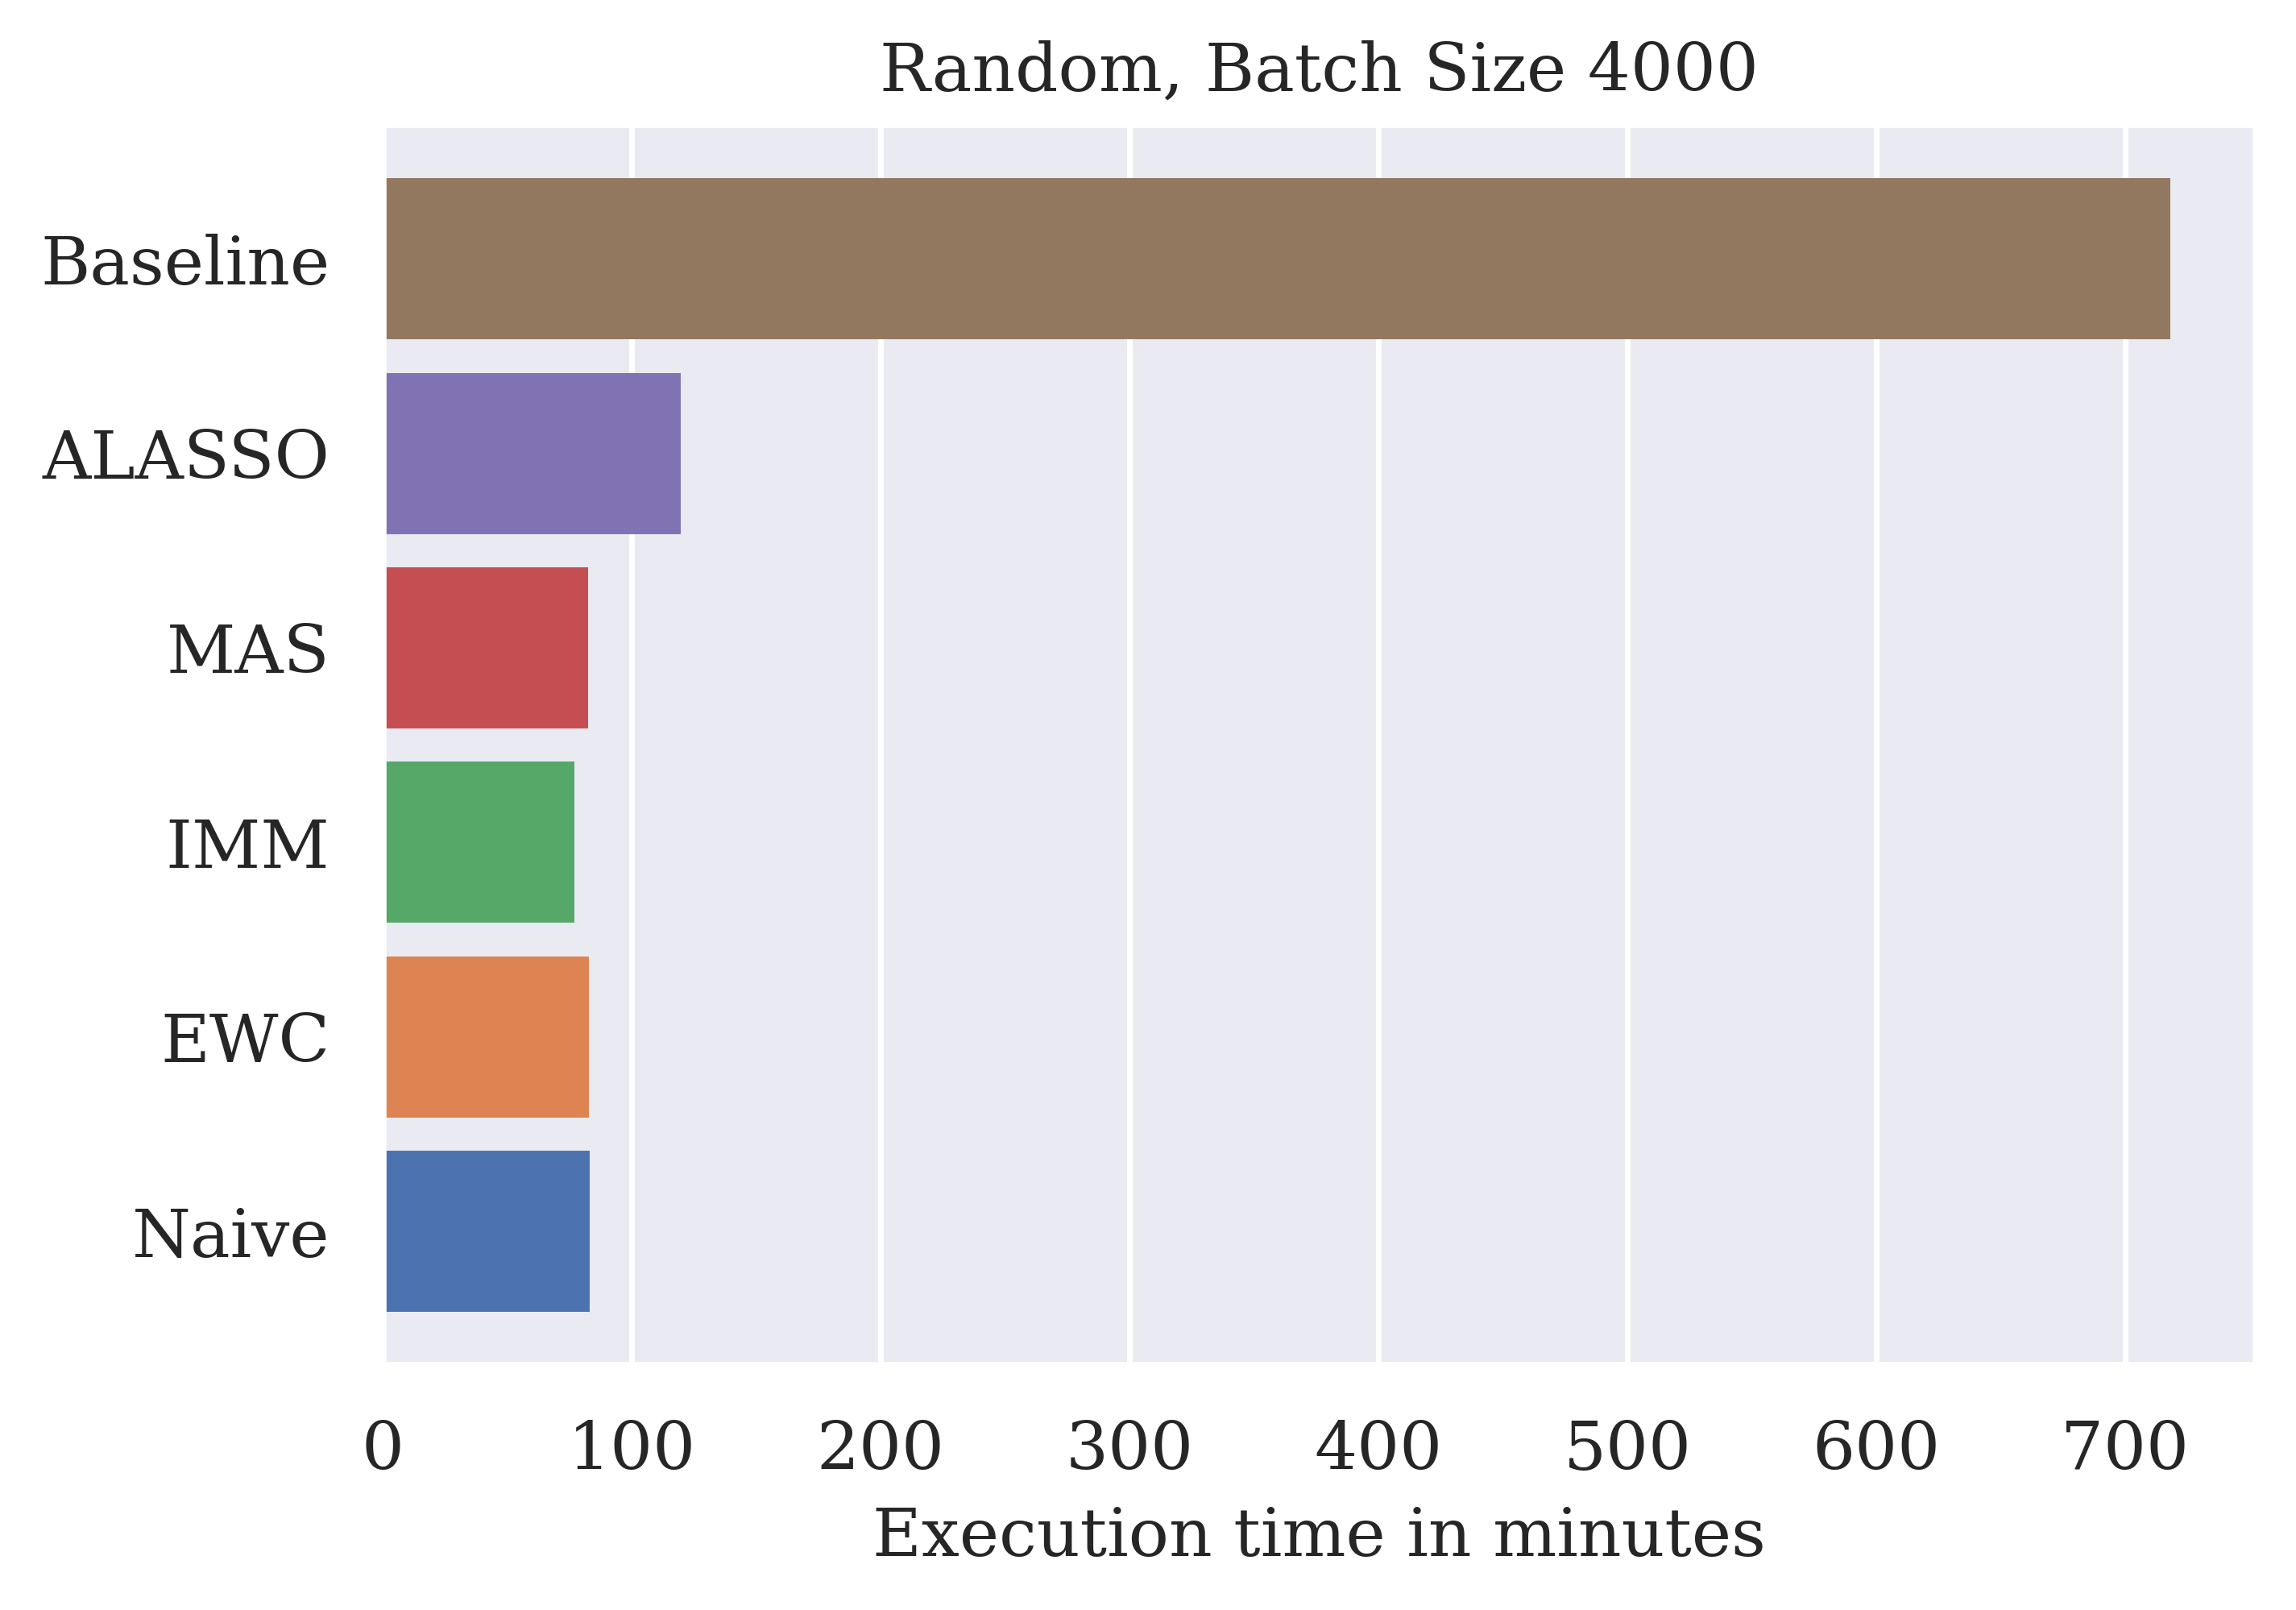
\includegraphics[width=0.3\linewidth]{images/results_CAL/random_4000b_time.png} \hfill
    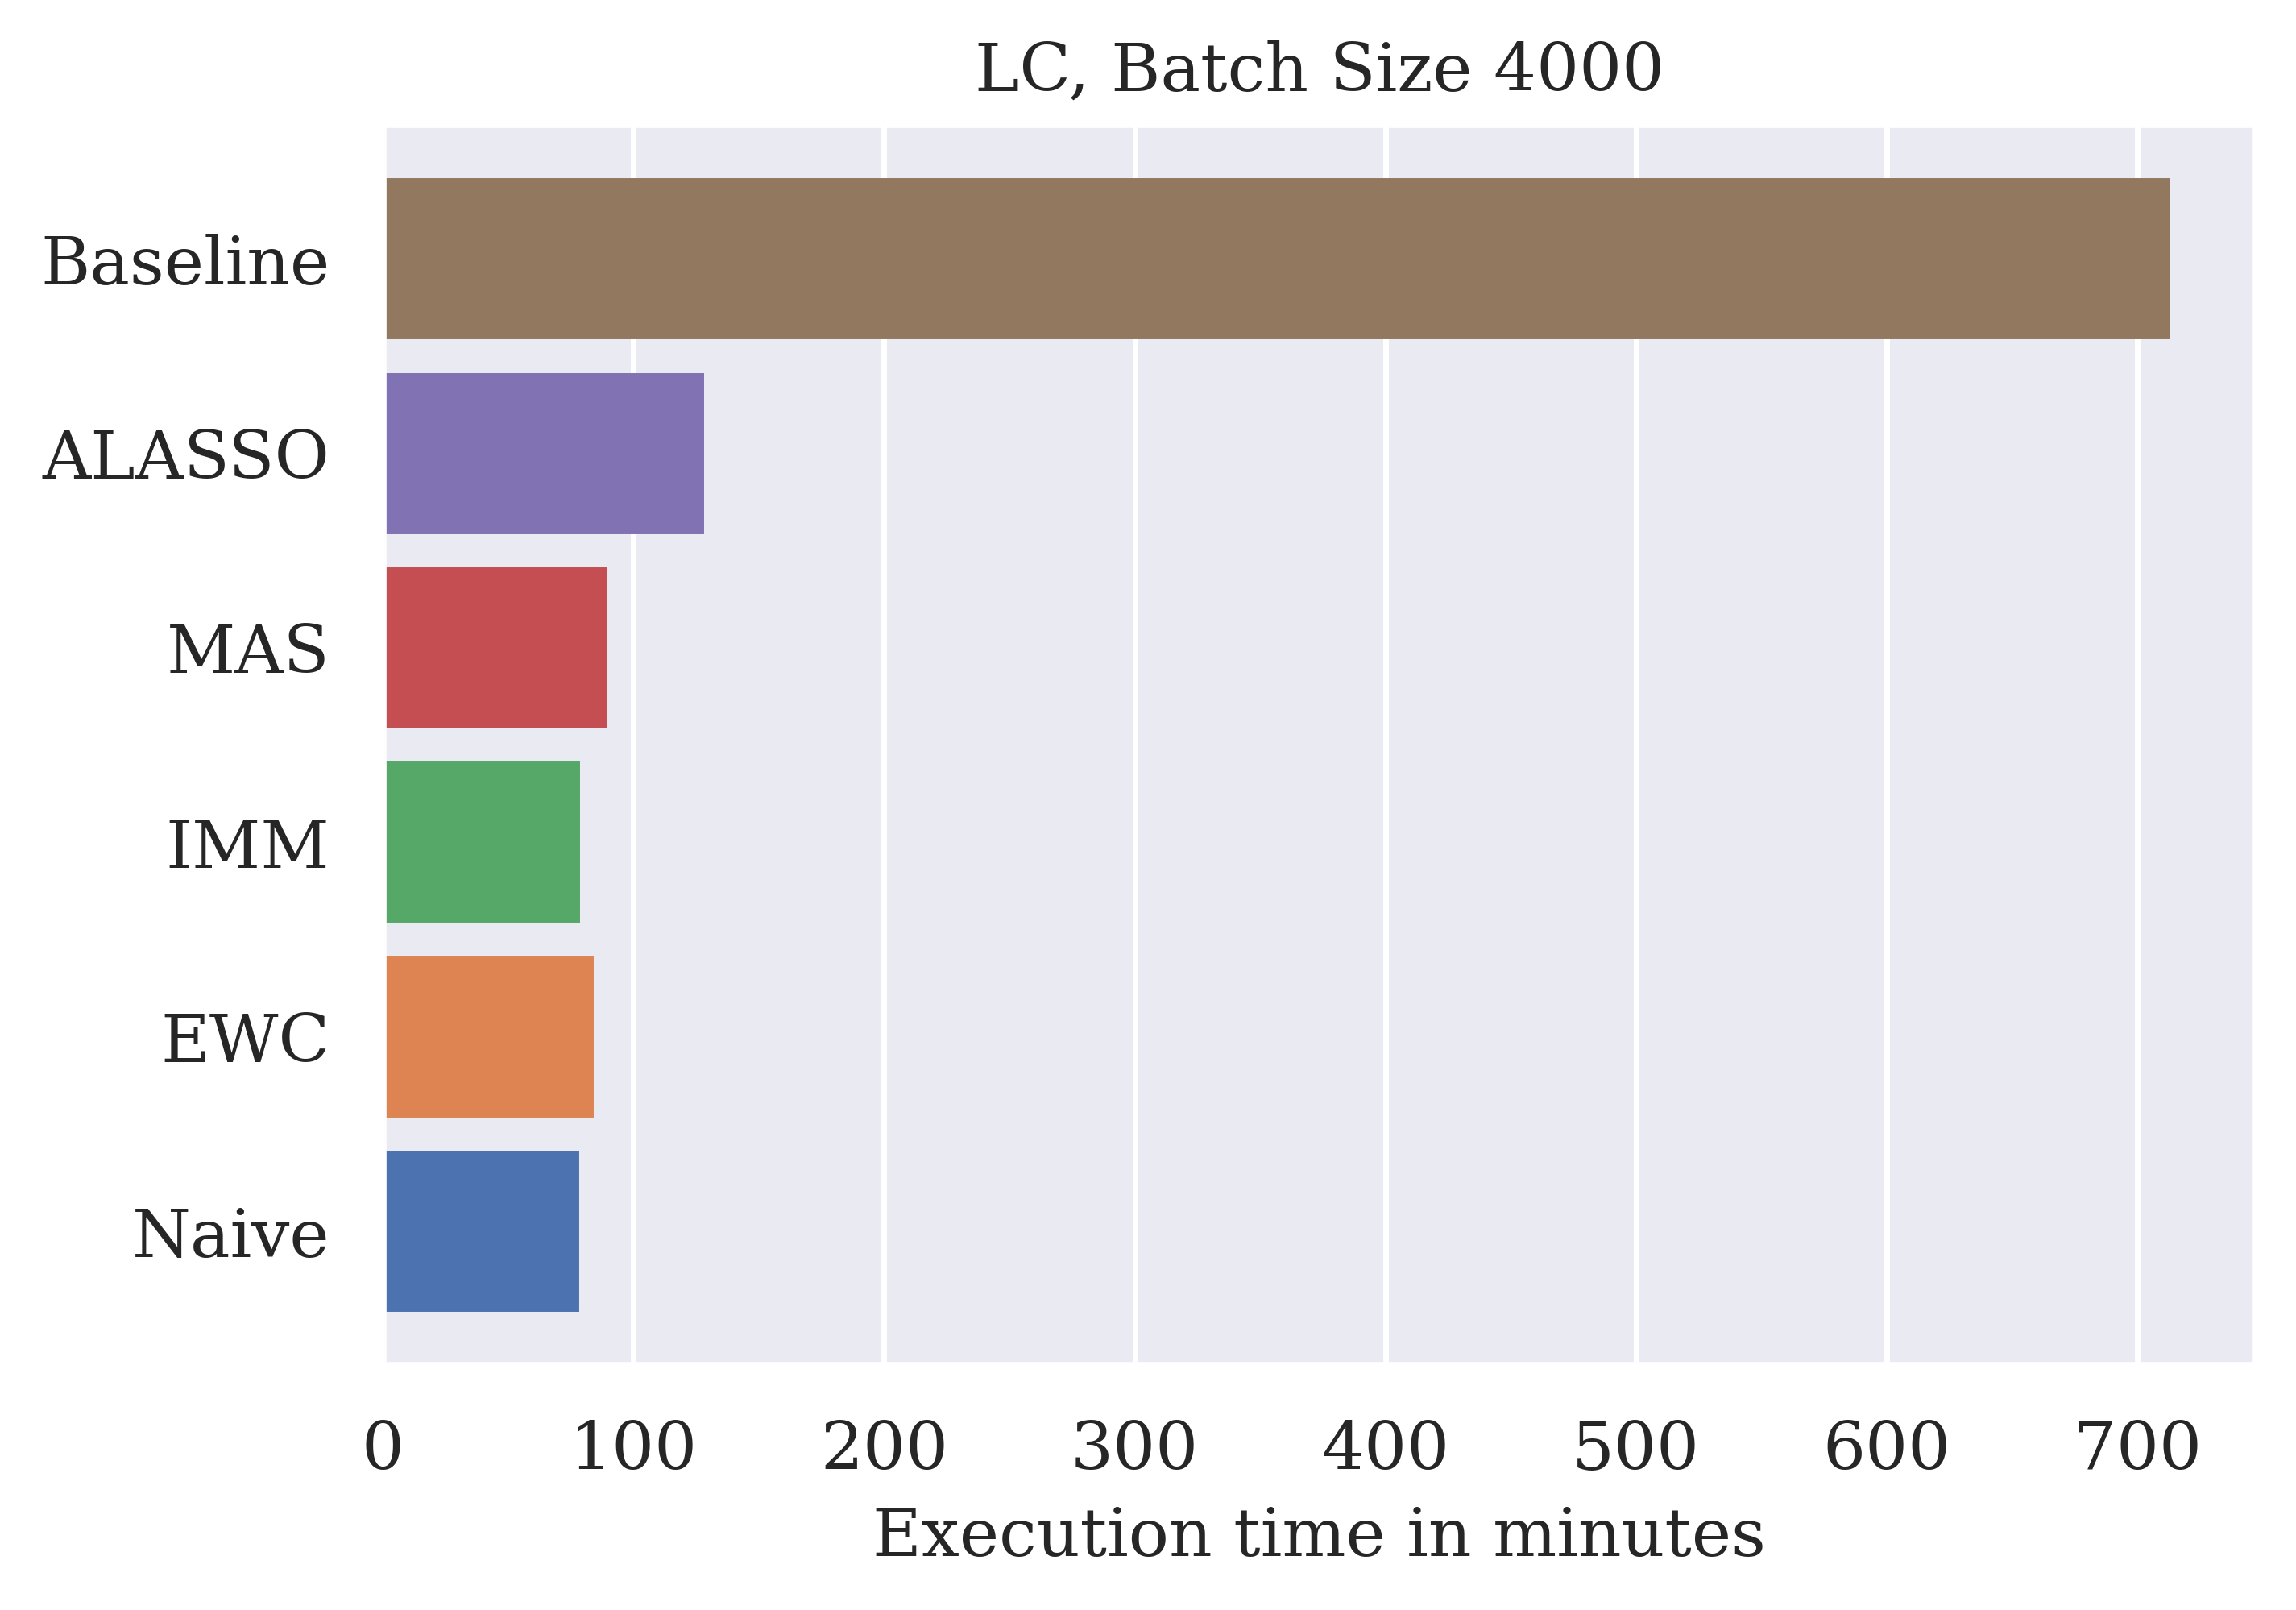
\includegraphics[width=0.3\linewidth]{images/results_CAL/lc_4000b_time.png} \hfill
    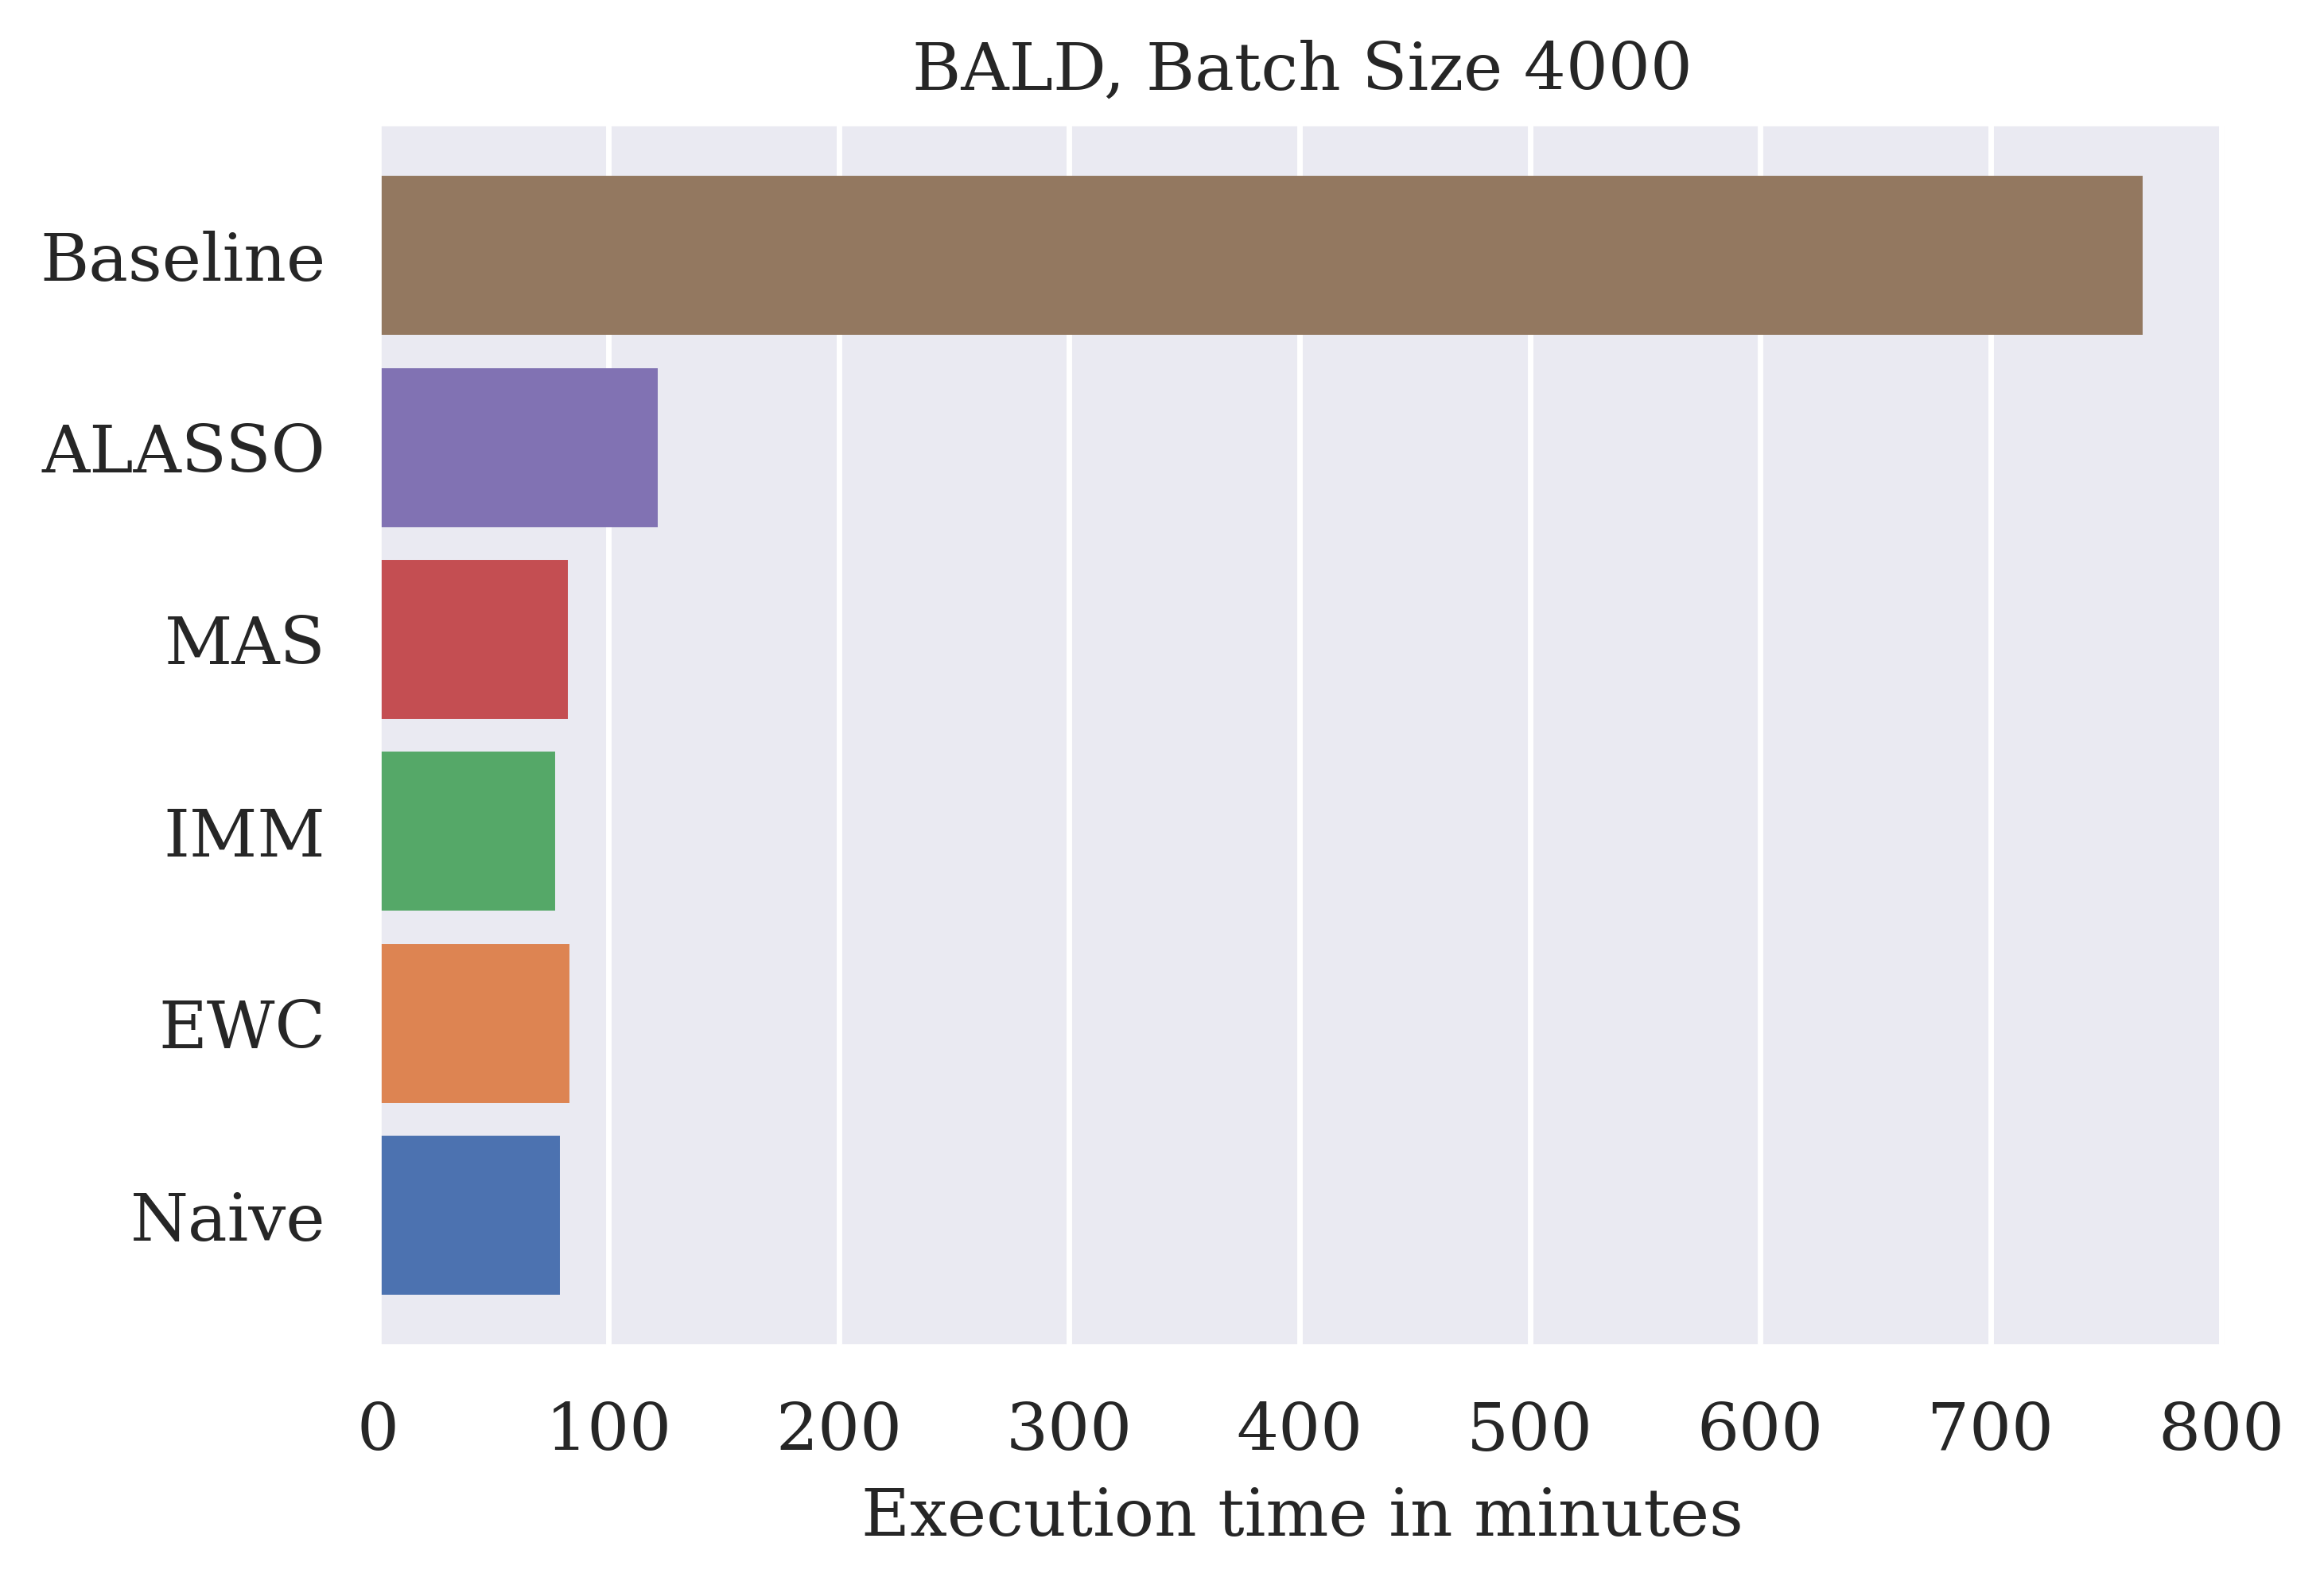
\includegraphics[width=0.3\linewidth]{images/results_CAL/bald_4000b_time.png}
    \\[\smallskipamount]
    \hfill 
    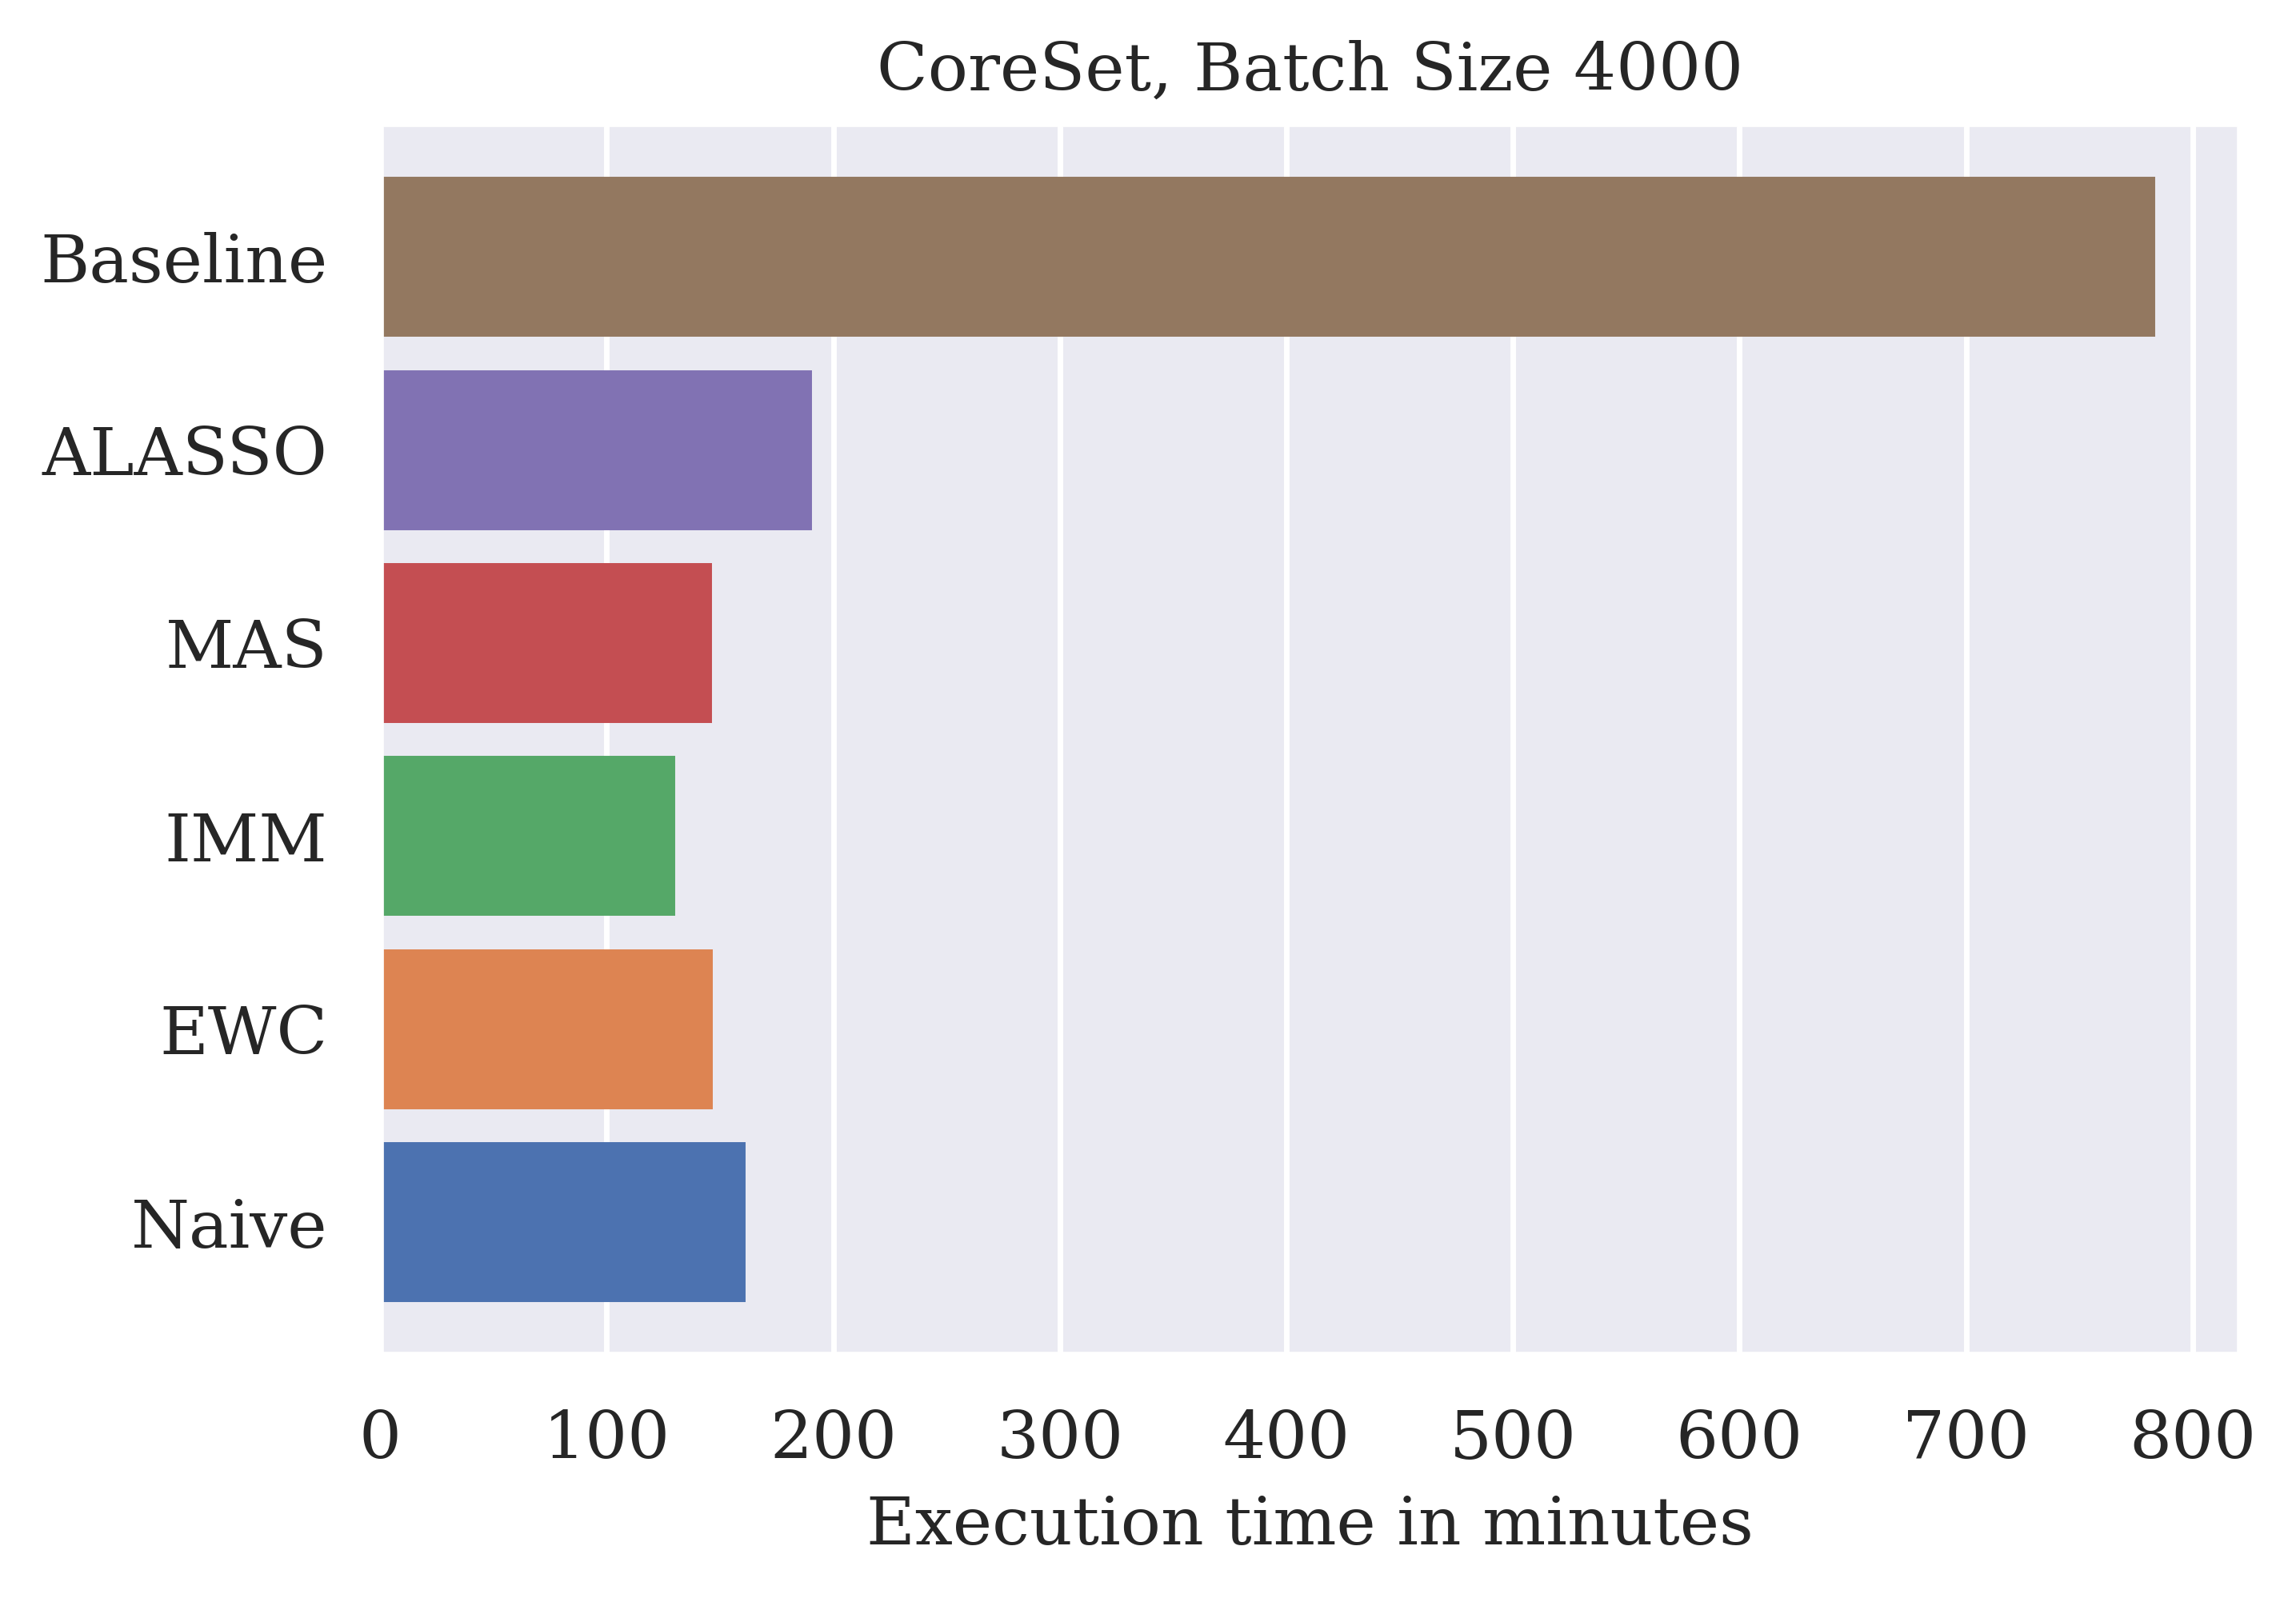
\includegraphics[width=0.3\linewidth]{images/results_CAL/coreset_4000b_time.png} \hfill
    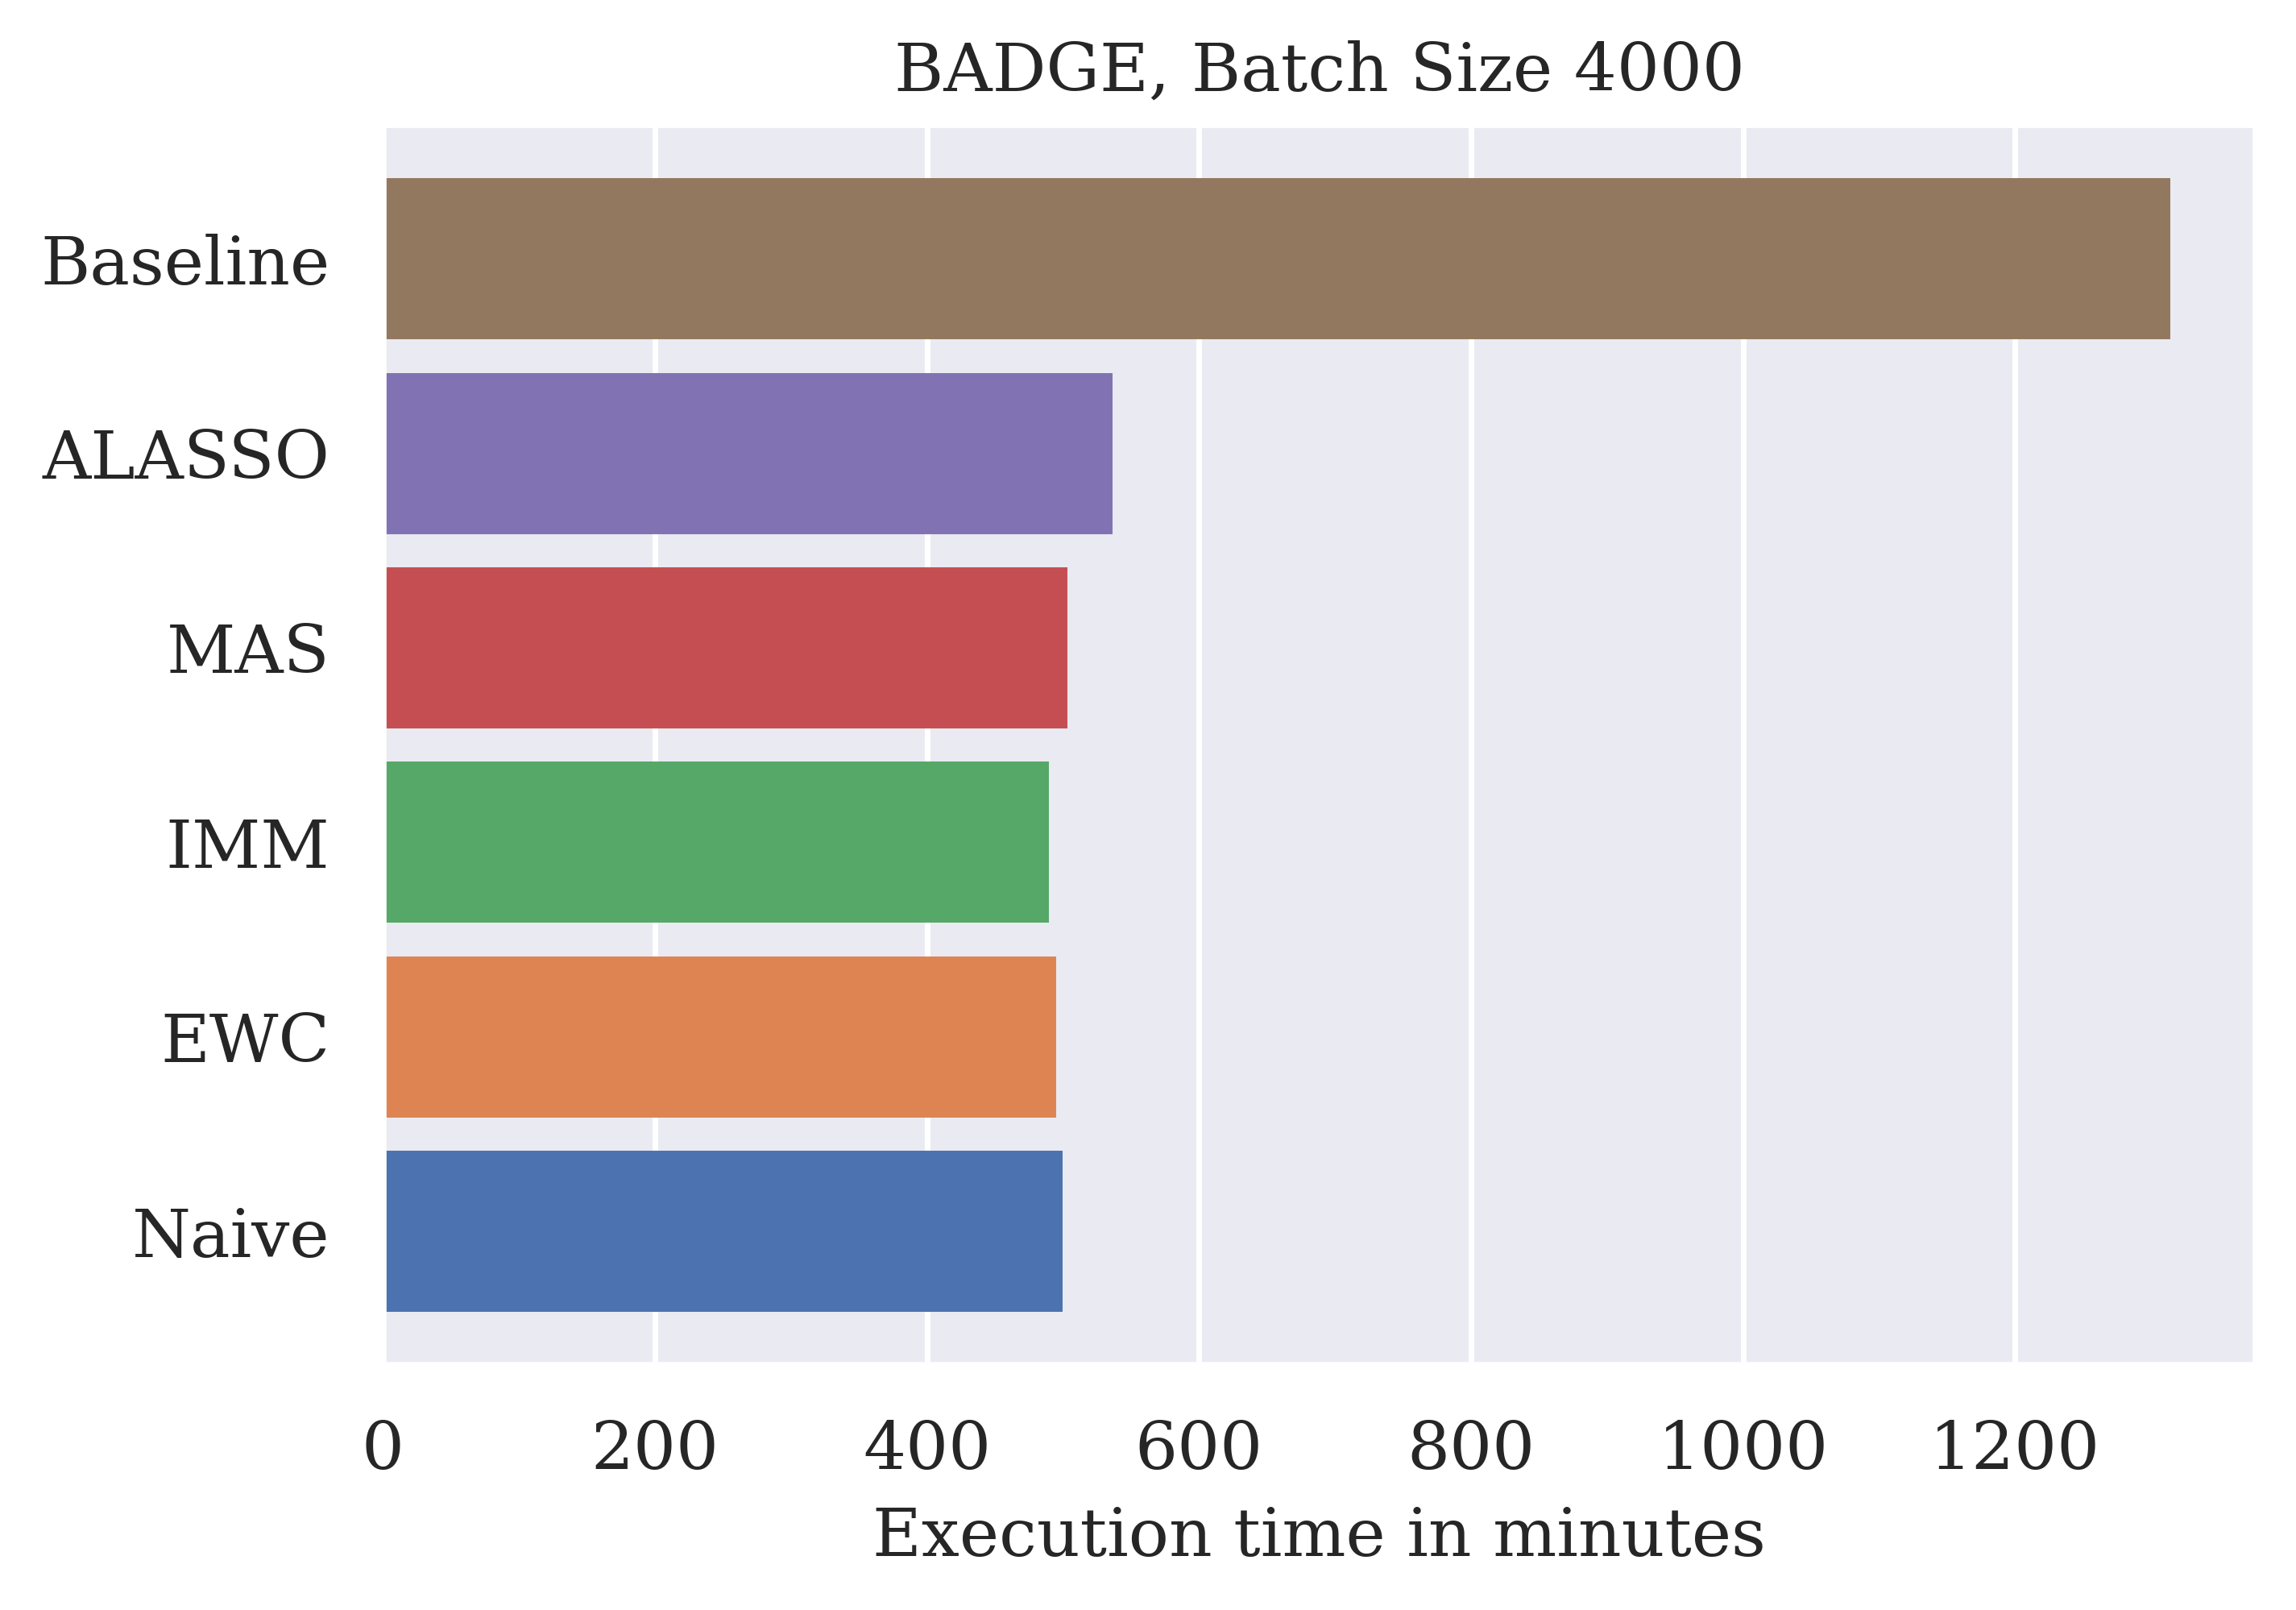
\includegraphics[width=0.3\linewidth]{images/results_CAL/badge_4000b_time.png} \hfill
    \caption[Continual Active Learning with \gls{badge} with varying batch size]{Comparison of execution time of Continual Learning and Active Learning strategies
    with batch size 4000.}
    \label{fig:Evaluation:Results:CAL:4000bTime}
\end{figure}



\begin{figure}[h]
    \centering
    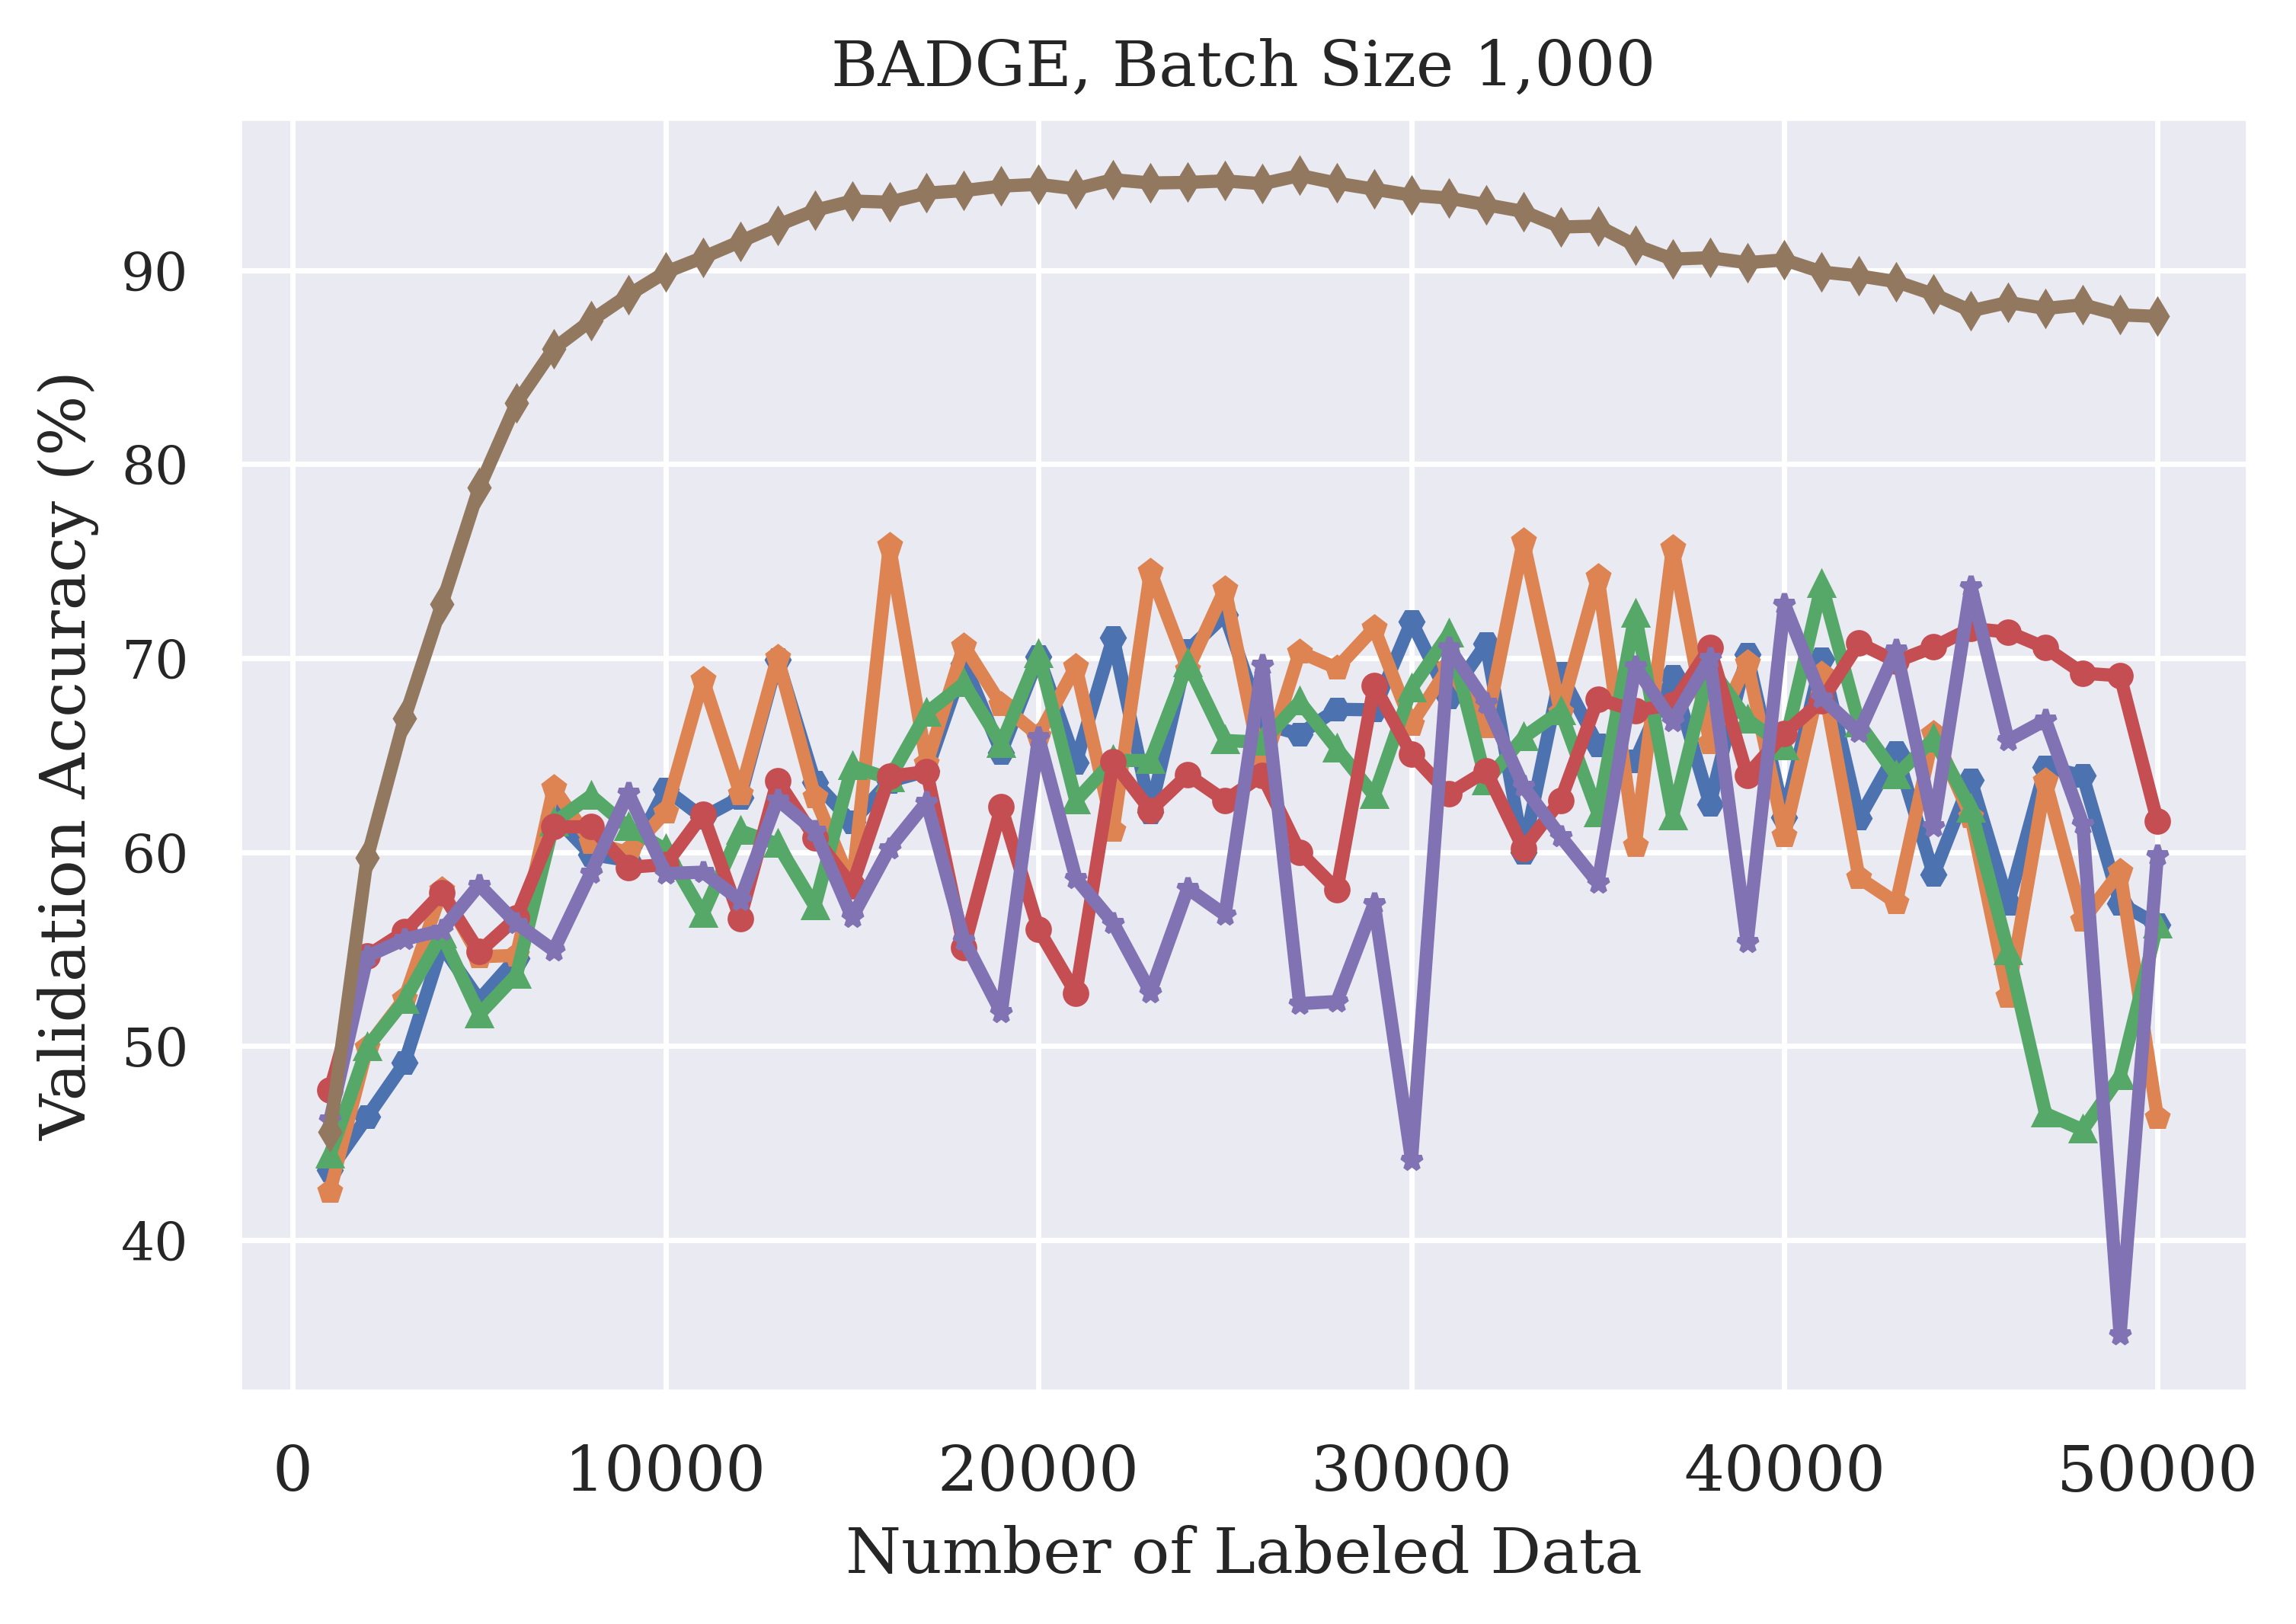
\includegraphics[width=0.3\linewidth]{images/results_CAL/badge_1000b_acc.png} \hfill
    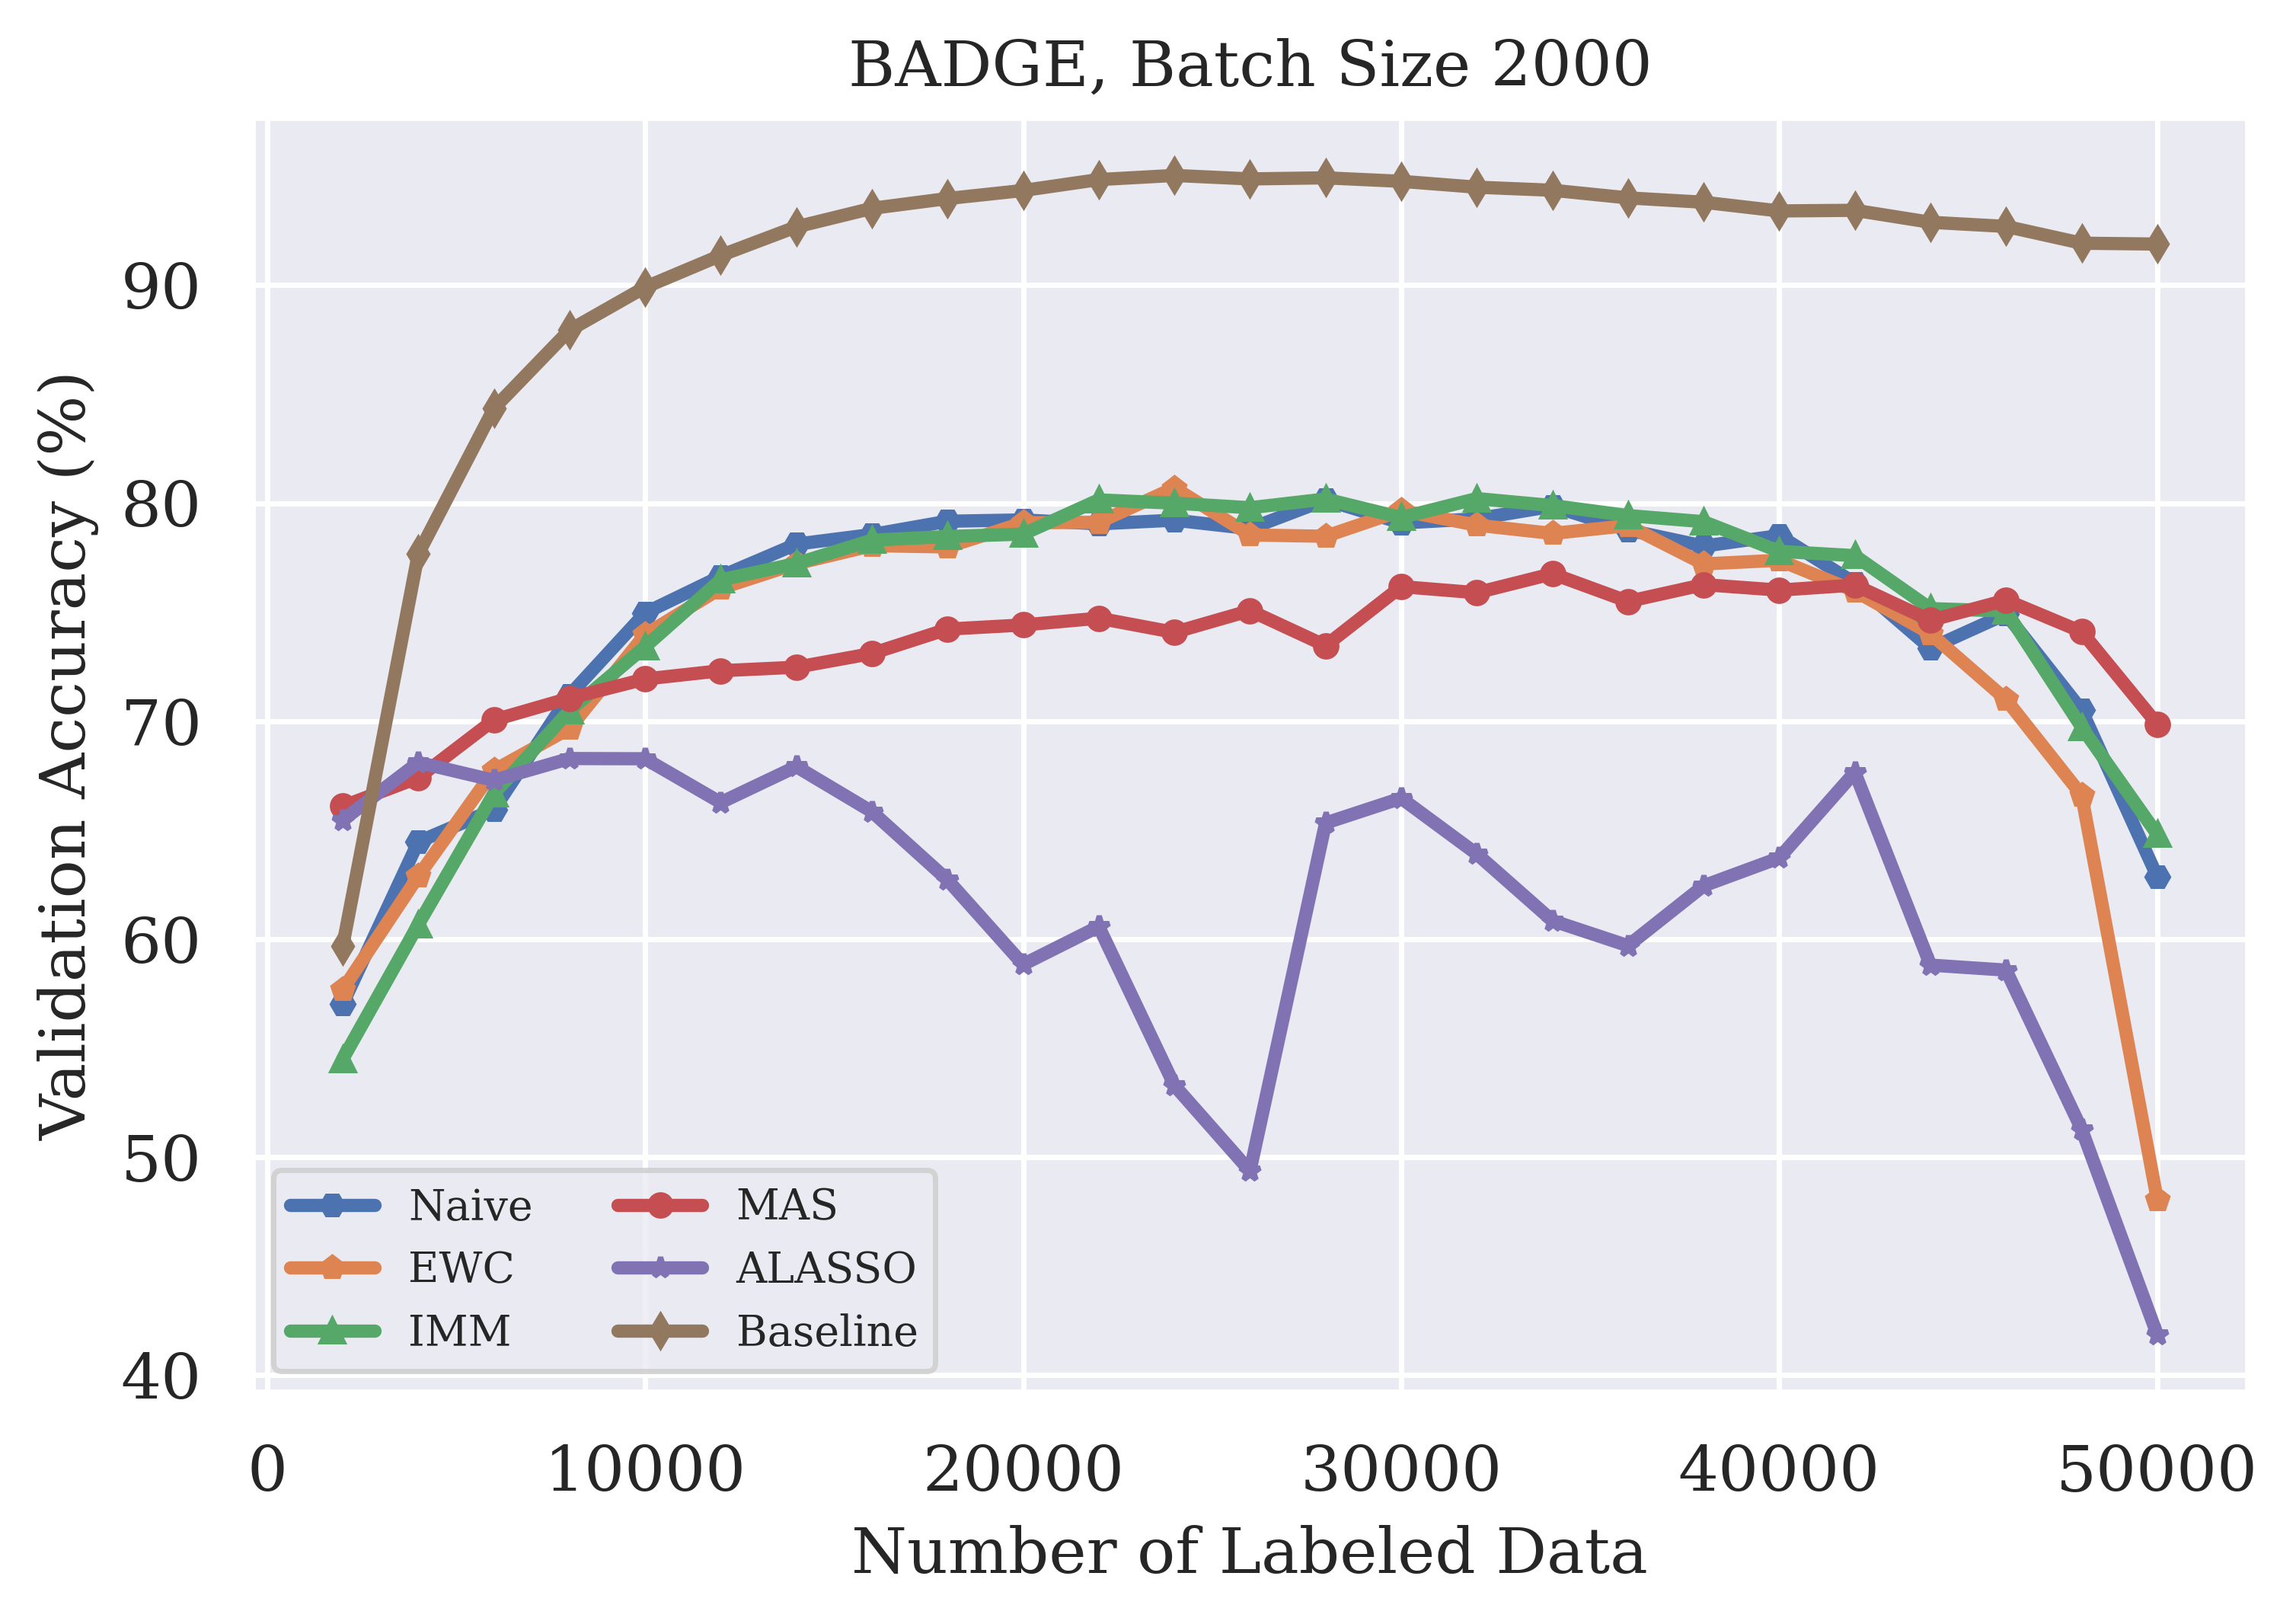
\includegraphics[width=0.3\linewidth]{images/results_CAL/badge_2000b_acc.png} \hfill
    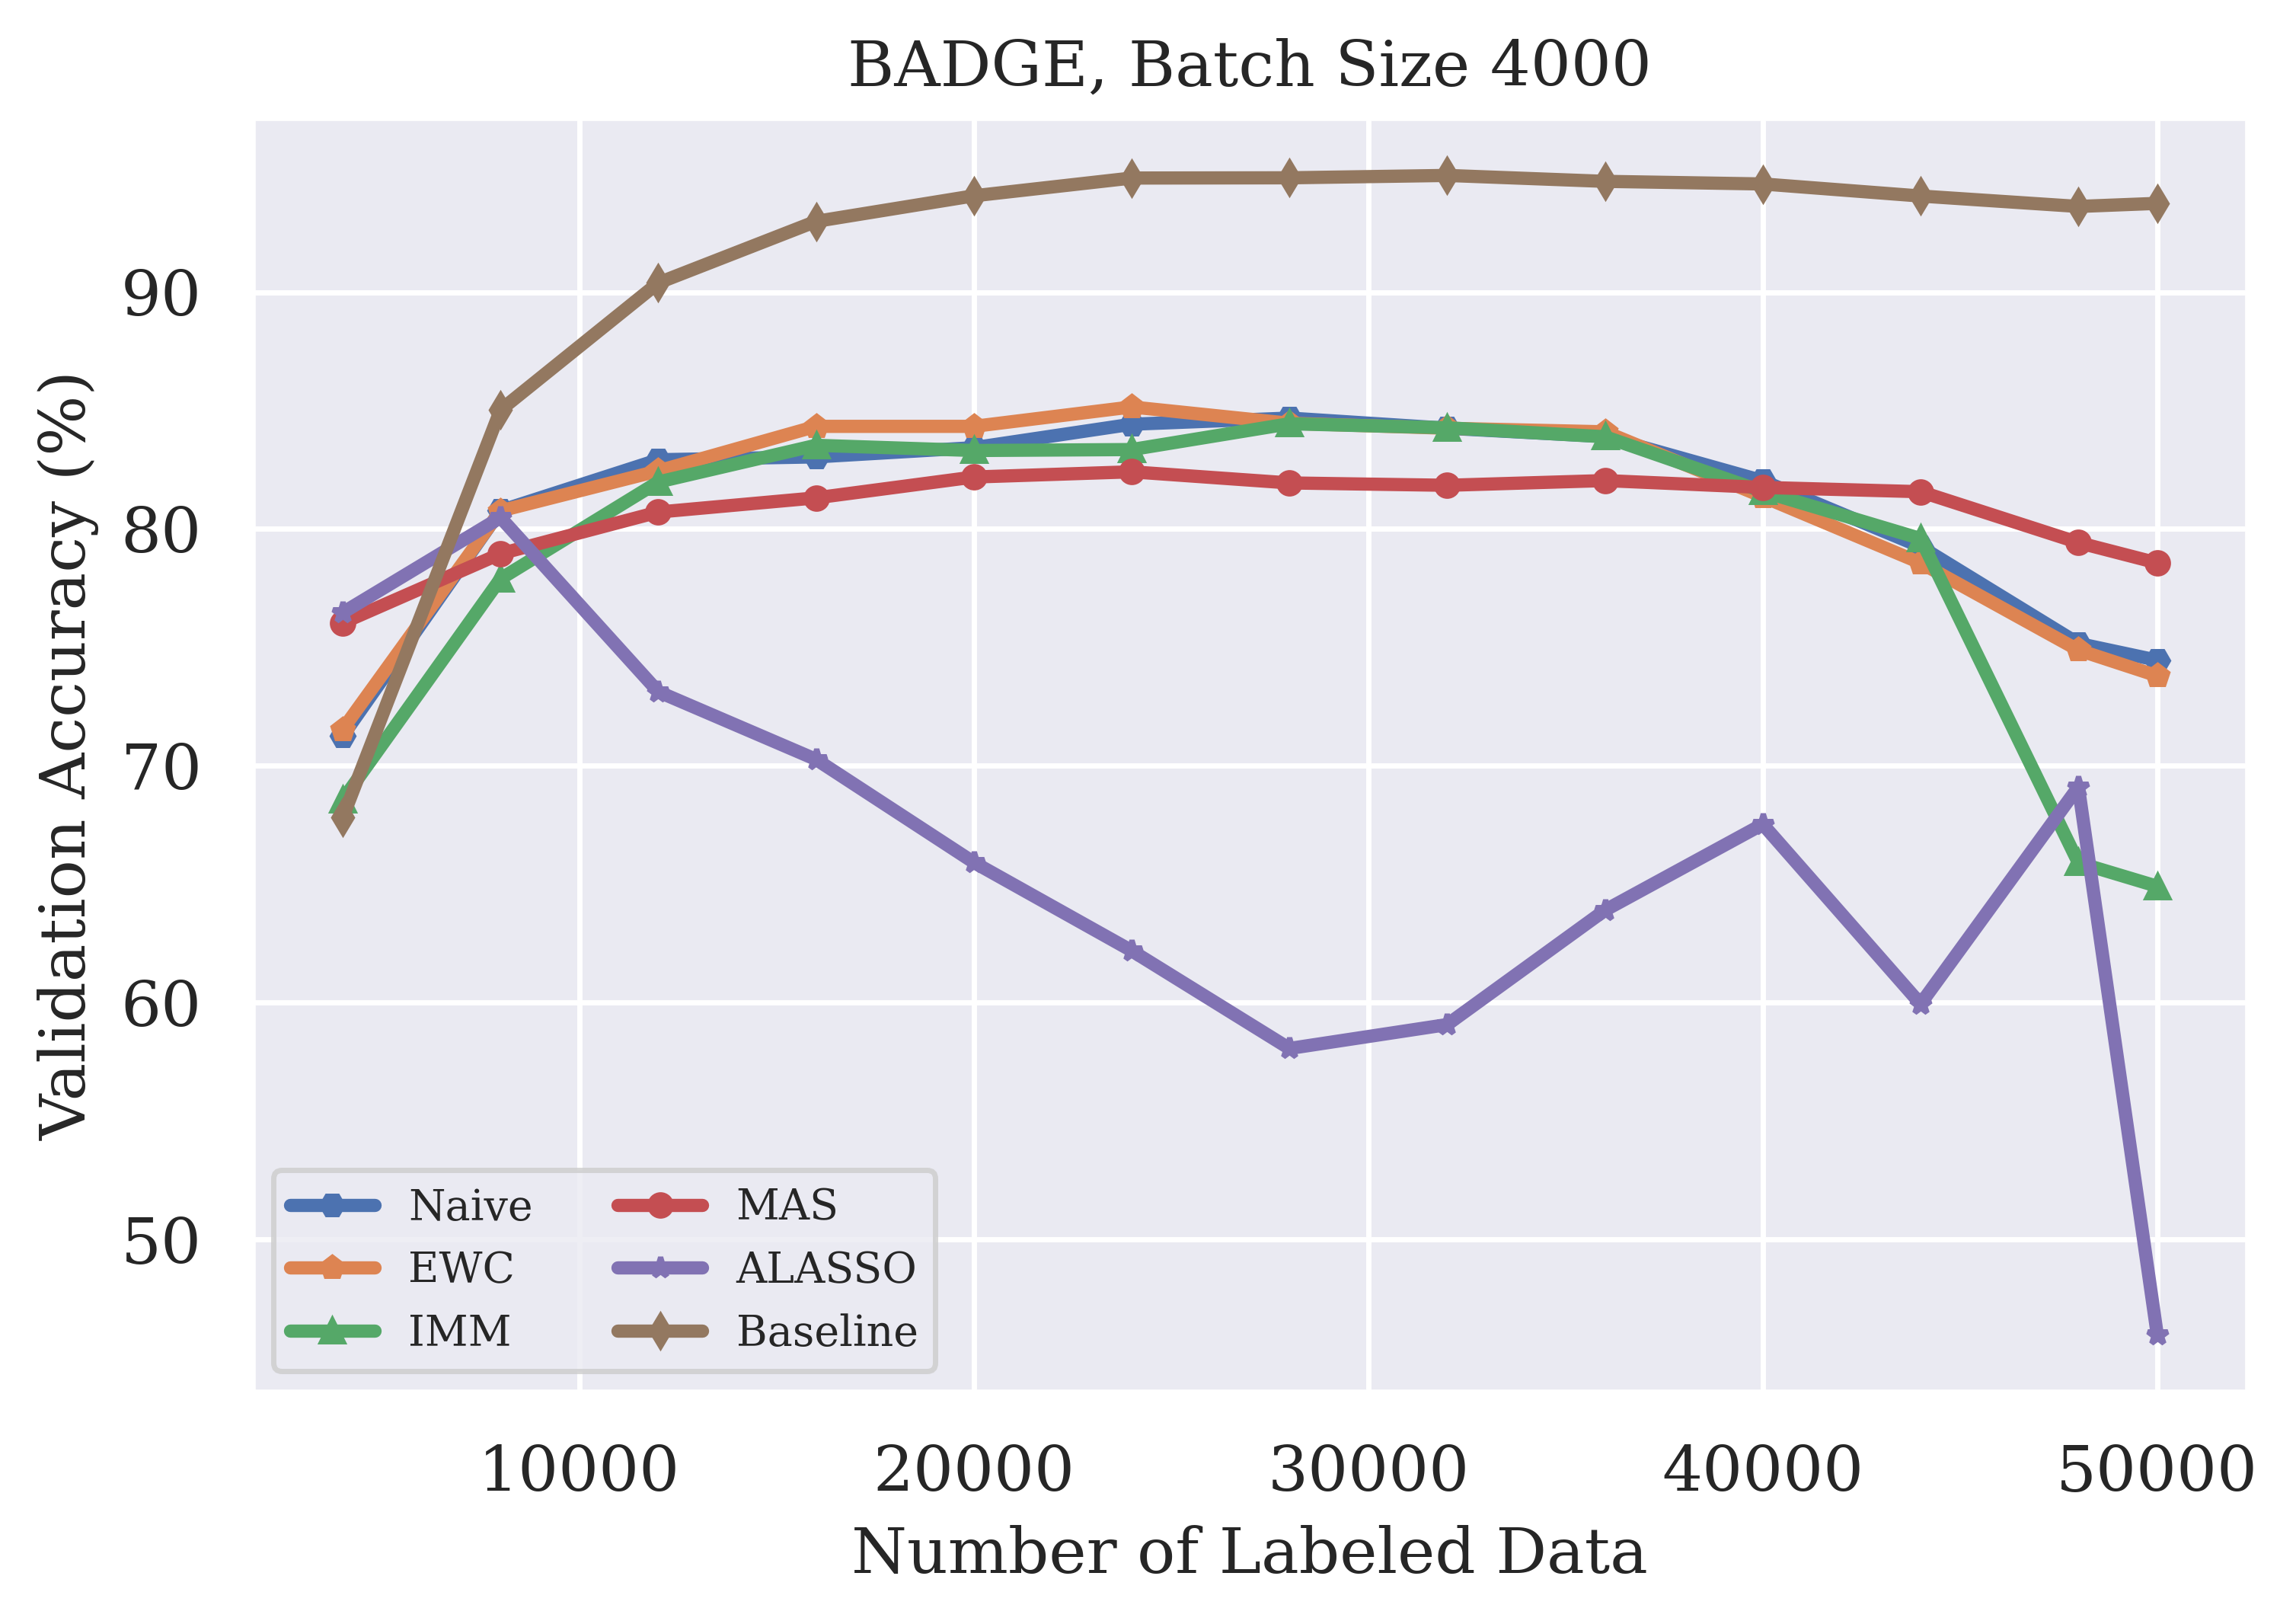
\includegraphics[width=0.3\linewidth]{images/results_CAL/badge_4000b_acc.png}
    \caption[Continual Active Learning with \gls{badge} with varying batch size]{Comparison of validation accuracy of Continual Learning strategies used with the Active Learning strategy
    \gls{badge}.}
    \label{fig:Evaluation:Results:CAL:VaryBatchSizeAcc}
\end{figure}

\begin{figure}[h]
    \centering
    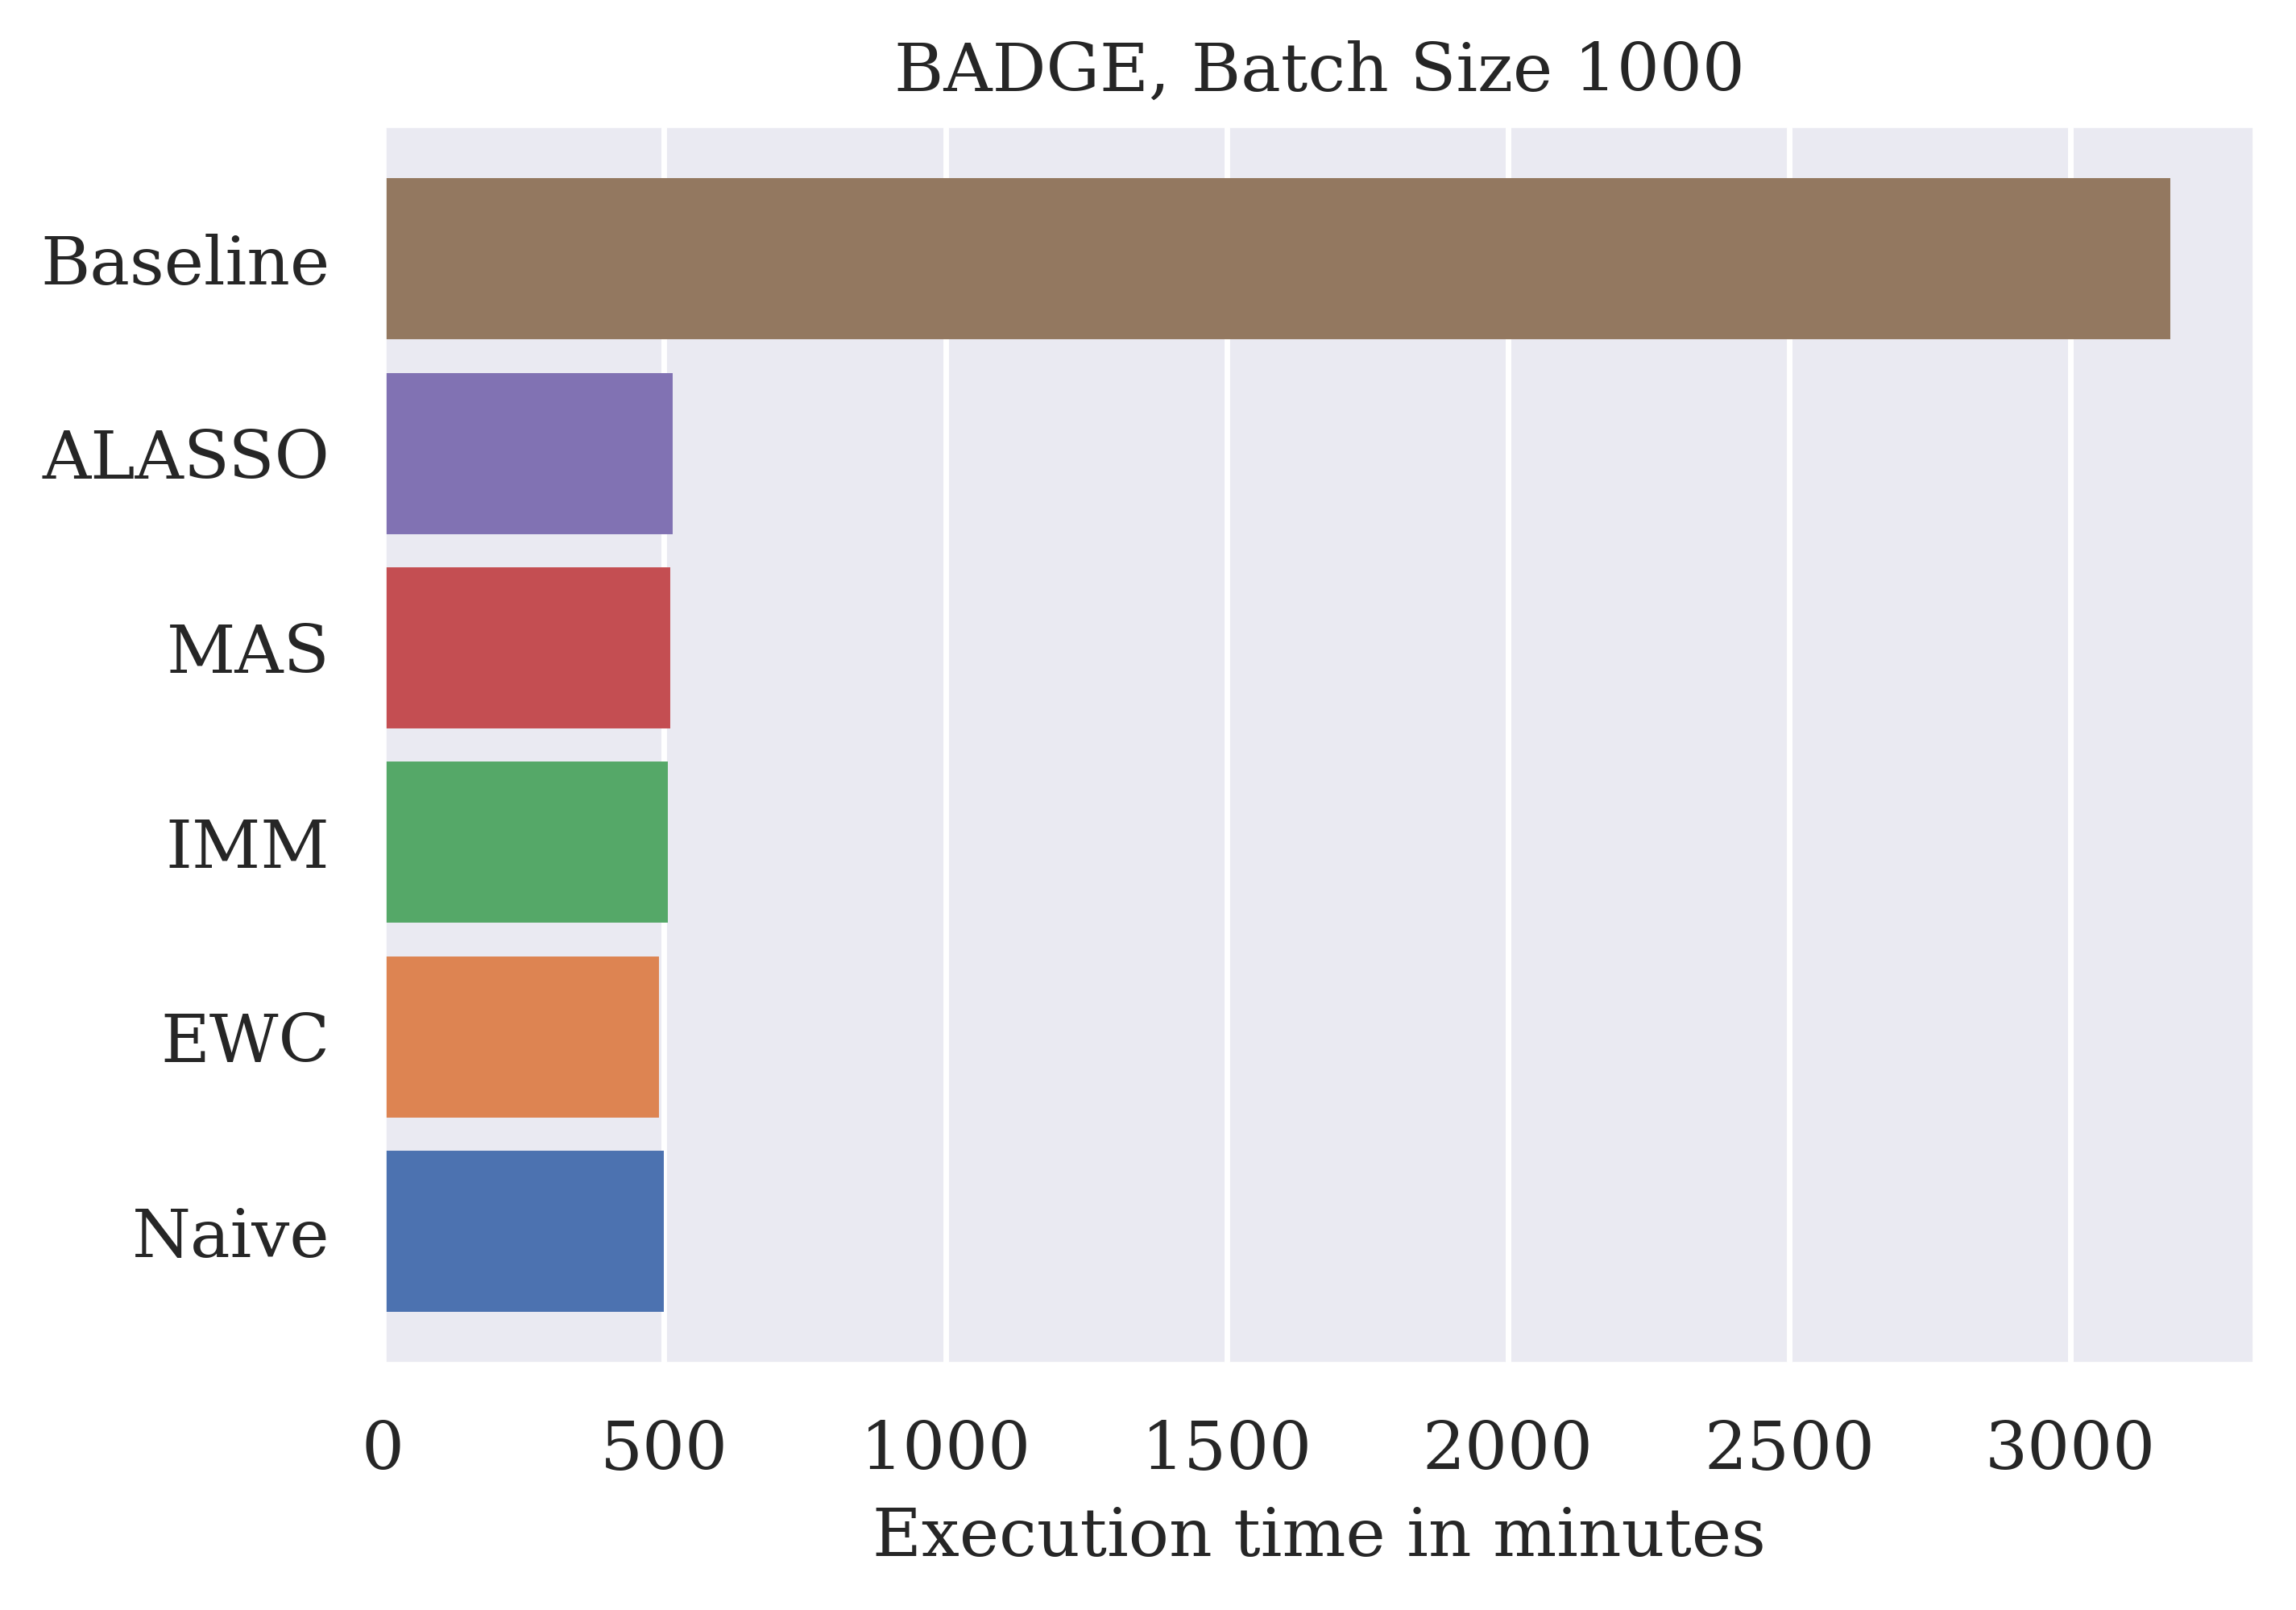
\includegraphics[width=0.3\linewidth]{images/results_CAL/badge_1000b_time.png} \hfill
    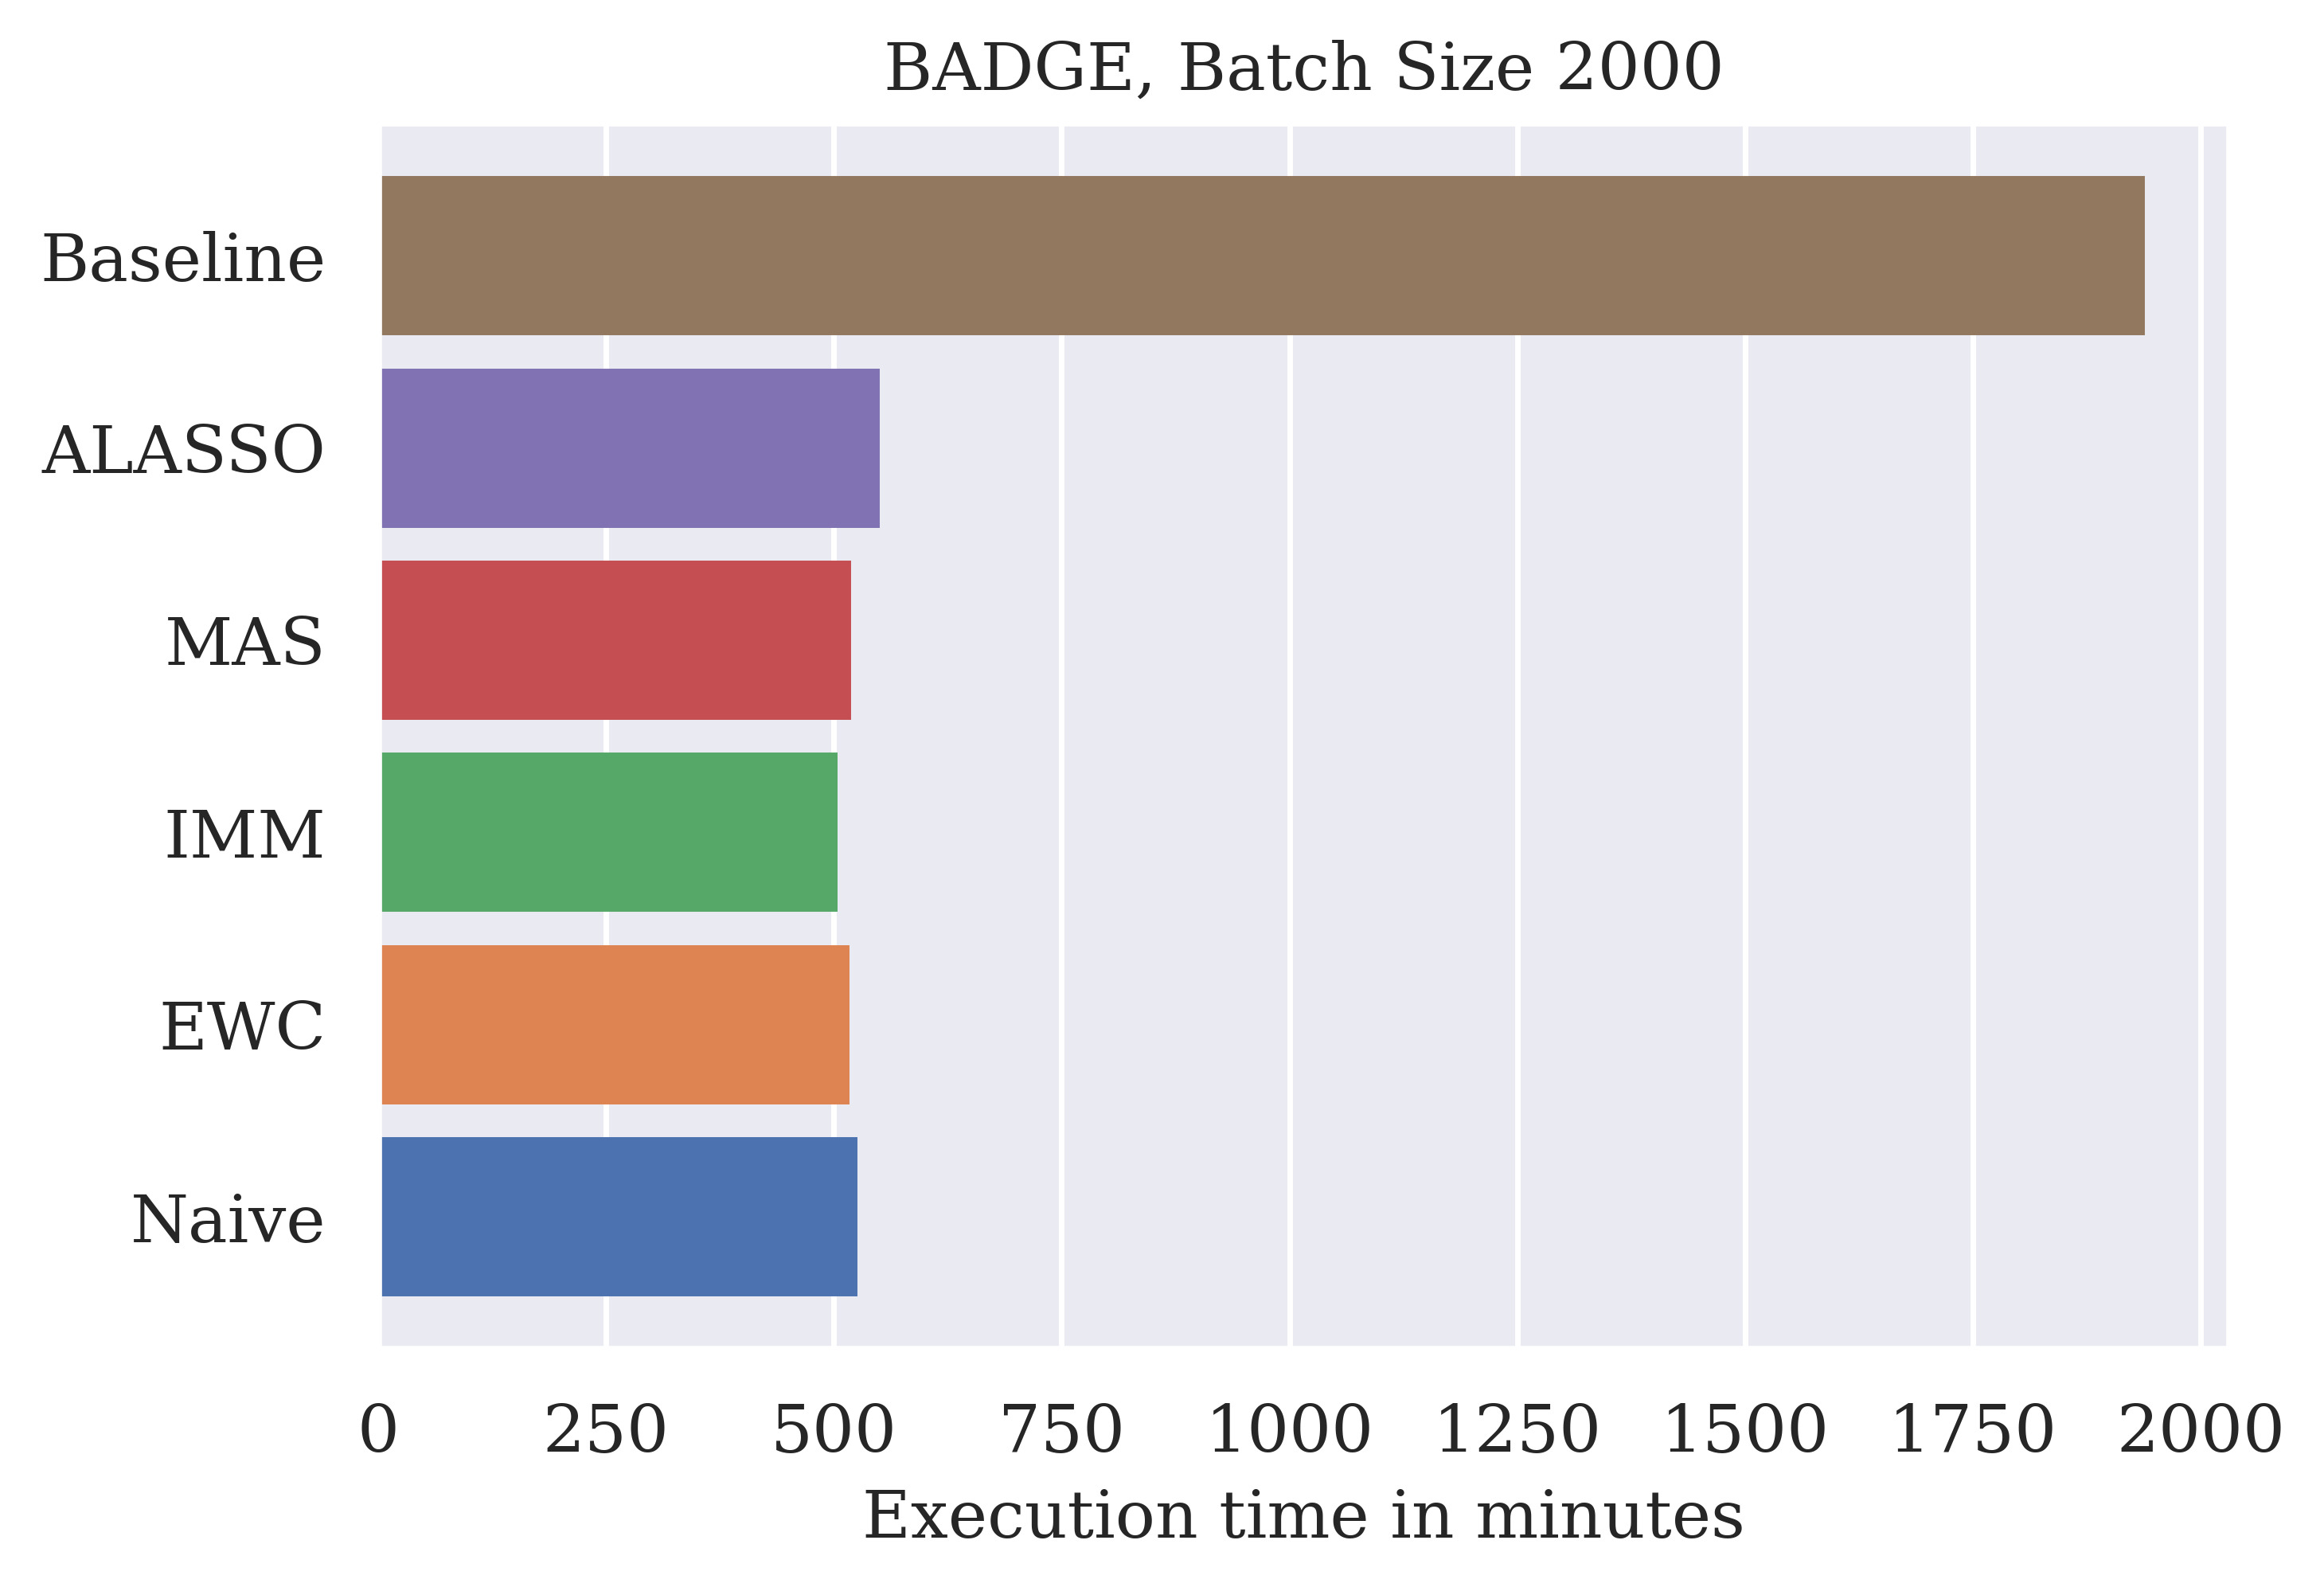
\includegraphics[width=0.3\linewidth]{images/results_CAL/badge_2000b_time.png} \hfill
    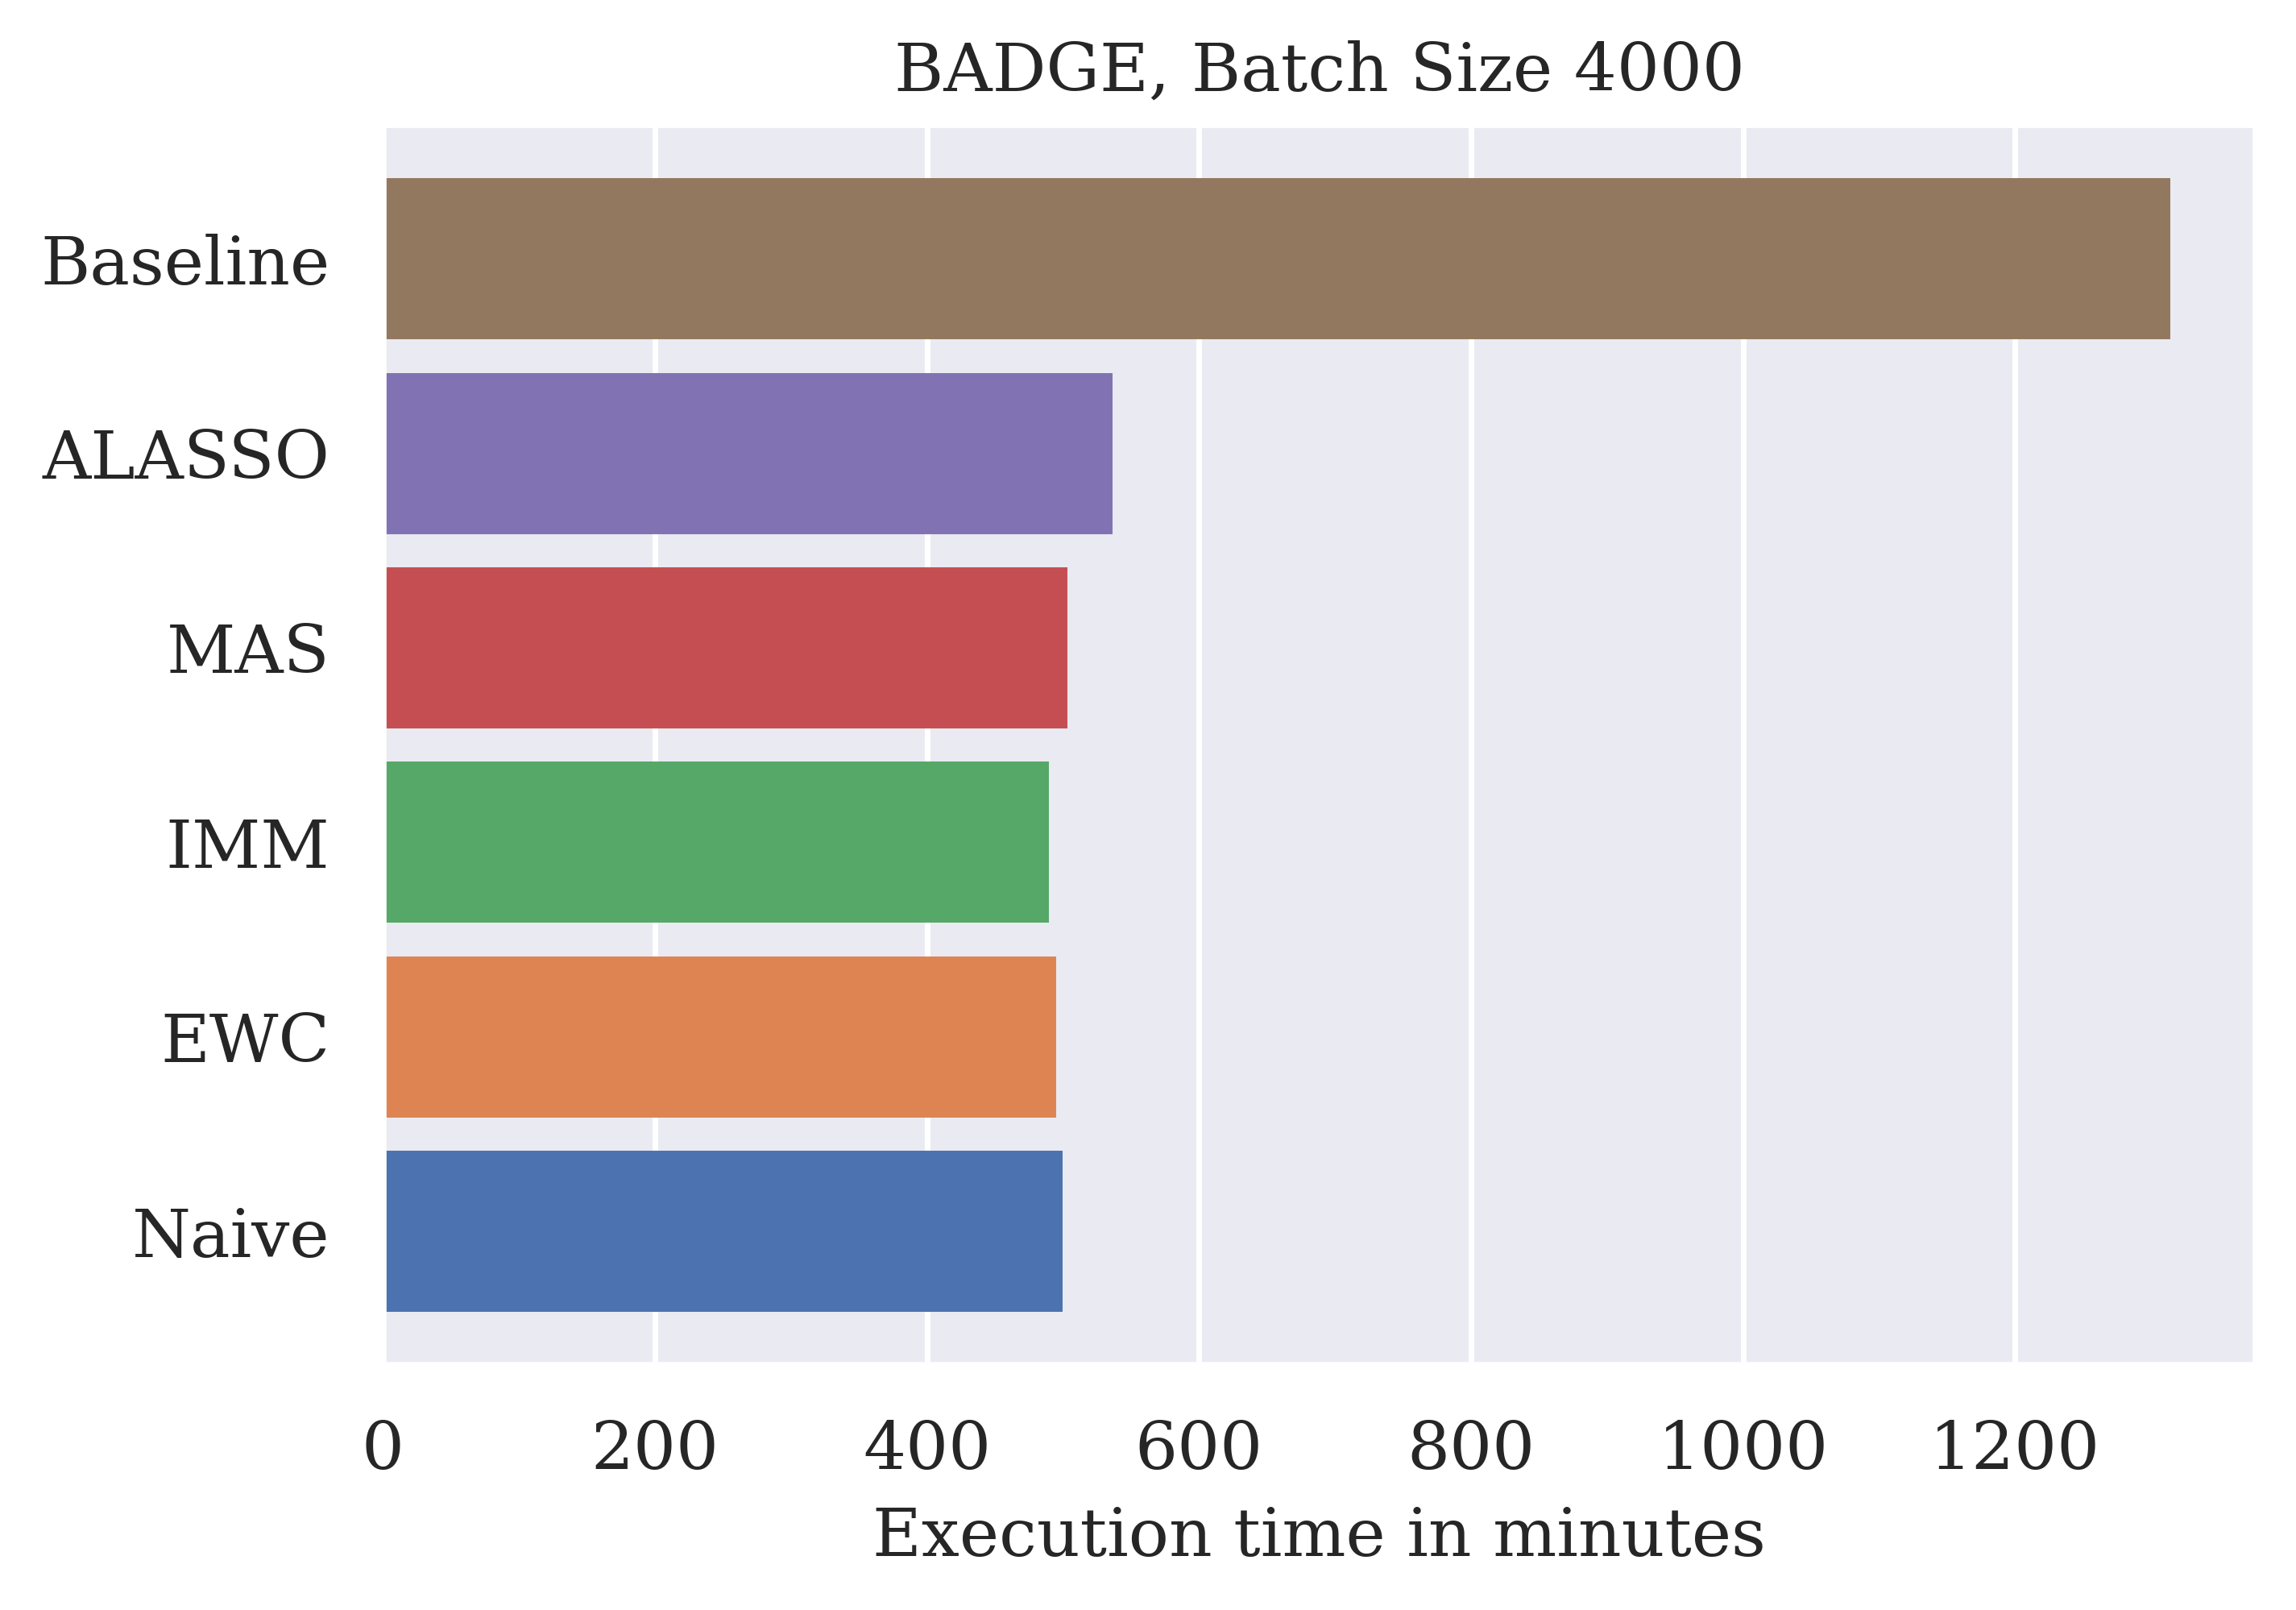
\includegraphics[width=0.3\linewidth]{images/results_CAL/badge_4000b_time.png}
    \caption[Continual Active Learning with \gls{badge} with varying batch size]{Comparison of validation accuracy of Continual Learning strategies used with the Active Learning strategy
    \gls{badge}.}
    \label{fig:Evaluation:Results:CAL:VaryBatchSizeTime}
\end{figure}

\subsubsection{A hybrid approach to Continual Learning}
\label{sec:Evaluation:Results:CAL:Hybrid}
After running the experiments in section \ref{sec:Evaluation:Results:CAL:ALCL}, we notice that all of them demonstrate a significant discrepancy in validation accuracy between Active Learning and Continual Active Learning. To further investigate this gap,
we investigate a hybrid approach where we run Active learning for the first $i$ iterations before switching to Continual Active Learning. With these experiments we hope to decrease the gap in validation accuracy to Active Learning. We vary $i$ between 0 and 6,
and perform two sets of experiments, one using the Continual Learning strategy \gls{mas} and the other using \gls{ewc}. In both experiments, we use the Active Learning strategy \gls{badge}. The results of the two sets of experiments can be found in figure 
\ref{fig:Evaluation:Results:CAL:DelayedStart}. For \gls{mas} and \gls{ewc}, the validation accuracy drops immediately after switching from Active Learning to Continual Active Learning. However, in the long run the \gls{mas} strategy retains the validation accuracy better than \gls{ewc}.
We also notice that while the validation accuracy does drop after switching to Continual Active Learning, it is higher at a fixed cycle than when switching to Continual Active Learning in an earlier cycle. \par

\begin{figure}[h]
    \centering
    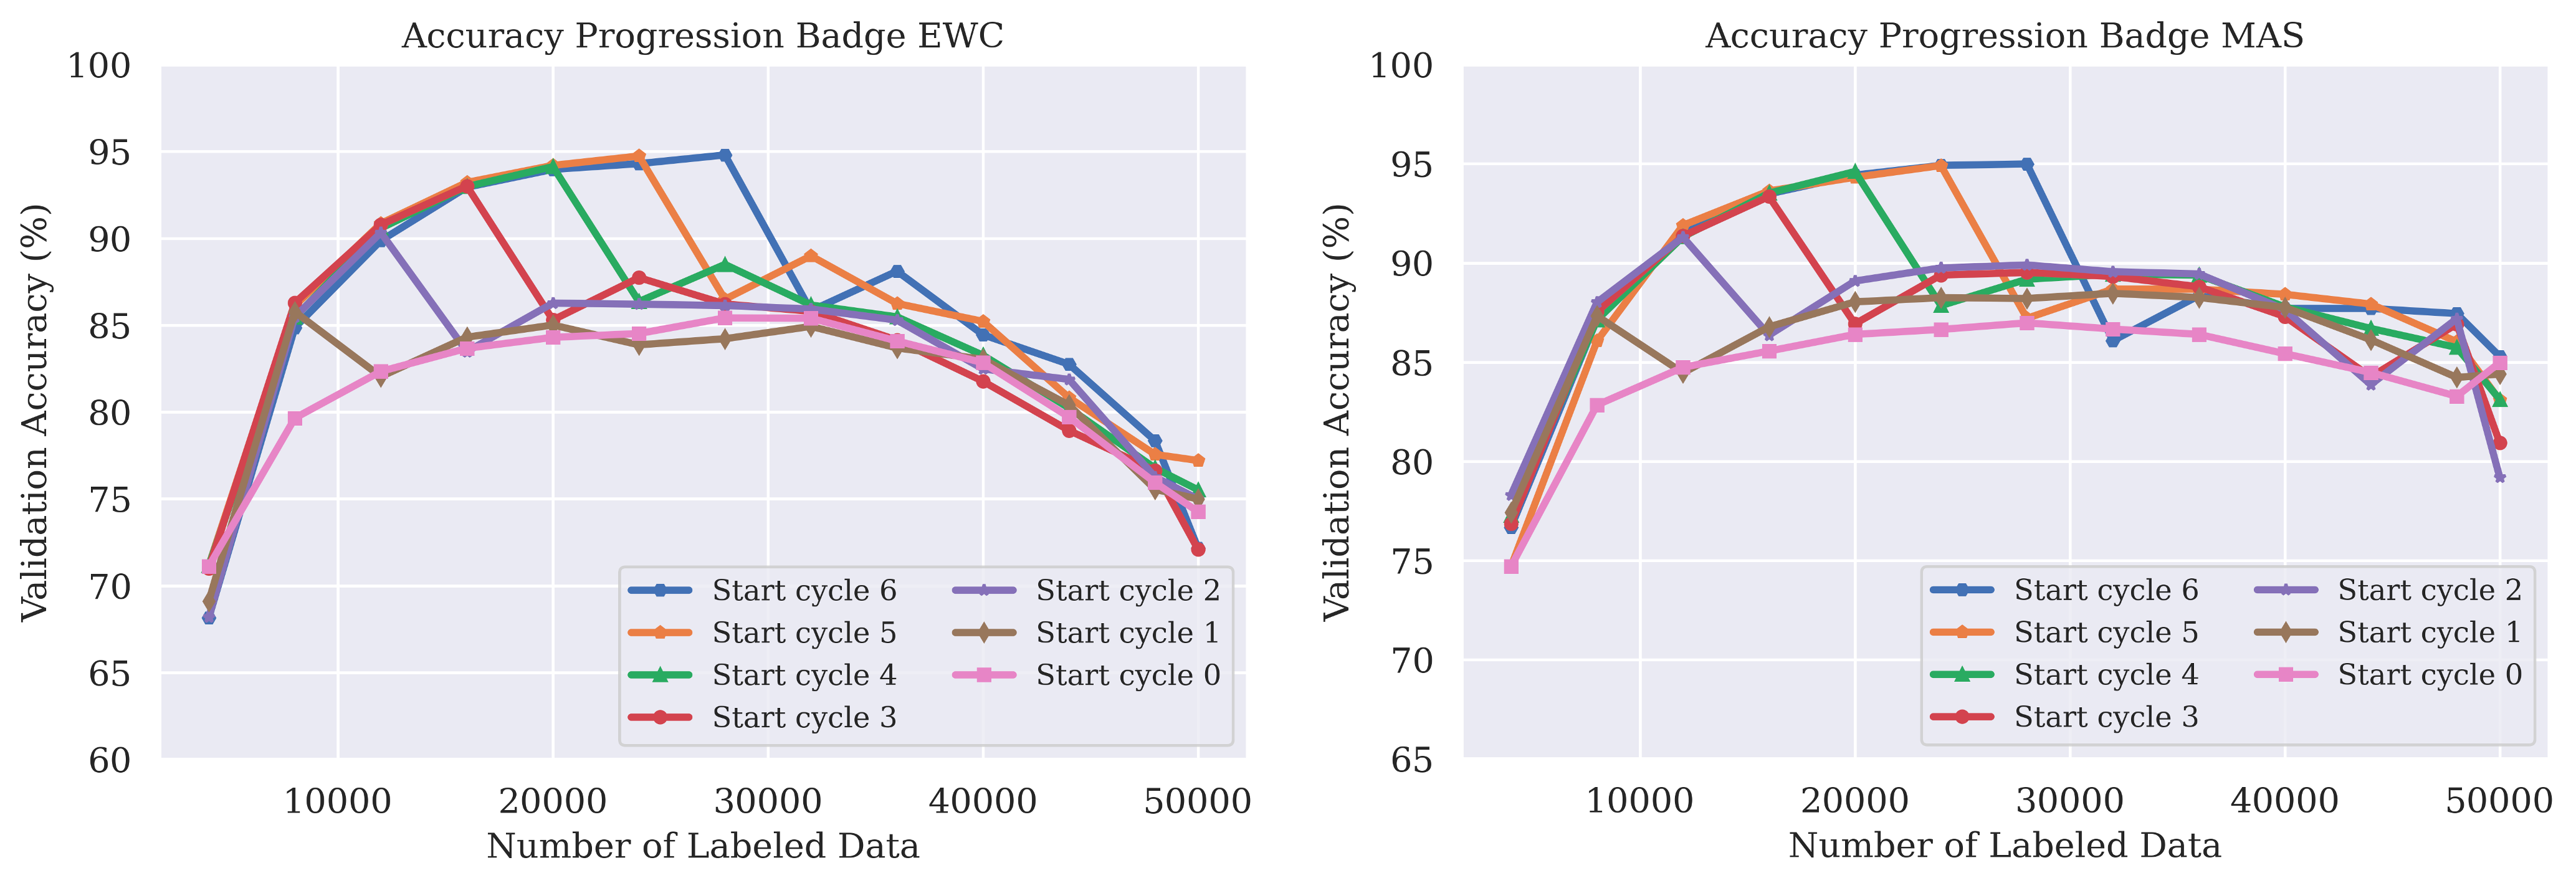
\includegraphics[width=\linewidth]{images/results_CAL/Delayed_start_CAL.png}
    \caption[Continual Active Learning Hybrid approach]{Comparison of validation accuracy for a delayed start of Continual Learning. Left: Accuracy progression for \gls{badge} and \gls{ewc}. Right: Accuracy progression for \gls{badge} and \gls{mas}.}
    \label{fig:Evaluation:Results:CAL:DelayedStart}
\end{figure}

\subsubsection{Varying the initialization of the labeled pool}
\label{sec:Evaluation:Results:CAL:Initialization}
Motivated by the findings from the previous section, we wonder if the initialization of the labeled pool has an impact on the validation accuracy of the Continual Learning strategies. Beck et al.\cite{beck2021effective} show that using a facility location selection 
\cite{iyer2021submodular} yields better validation accuracy when training on the initial labeled pool. We therefore test the effect of an initialization using the facility location selection compared to our random initialization. As our Active Learning strategy,
we use \gls{badge} with a batch size of 4000 and \gls{mas} as our Continual Learning strategy. The results of the experiment can be found in figure \ref{fig:Evaluation:Results:CAL:FLinit}. While the facility location approach performs better than random initialization, the difference is
marginal. Interestingly, the validation accuracy of the facility location approach is lower than the random initialization in the first iteration. The most significant drawback of the facility location initialization is its resource-intensity. Initialization with facility
location takes about 24 hours to complete and requires more than 100GB of memory for CIFAR-10 using the implementation proposed by Beck et al. \cite{beck2021effective}. \par

\begin{figure}[h]
    \centering
    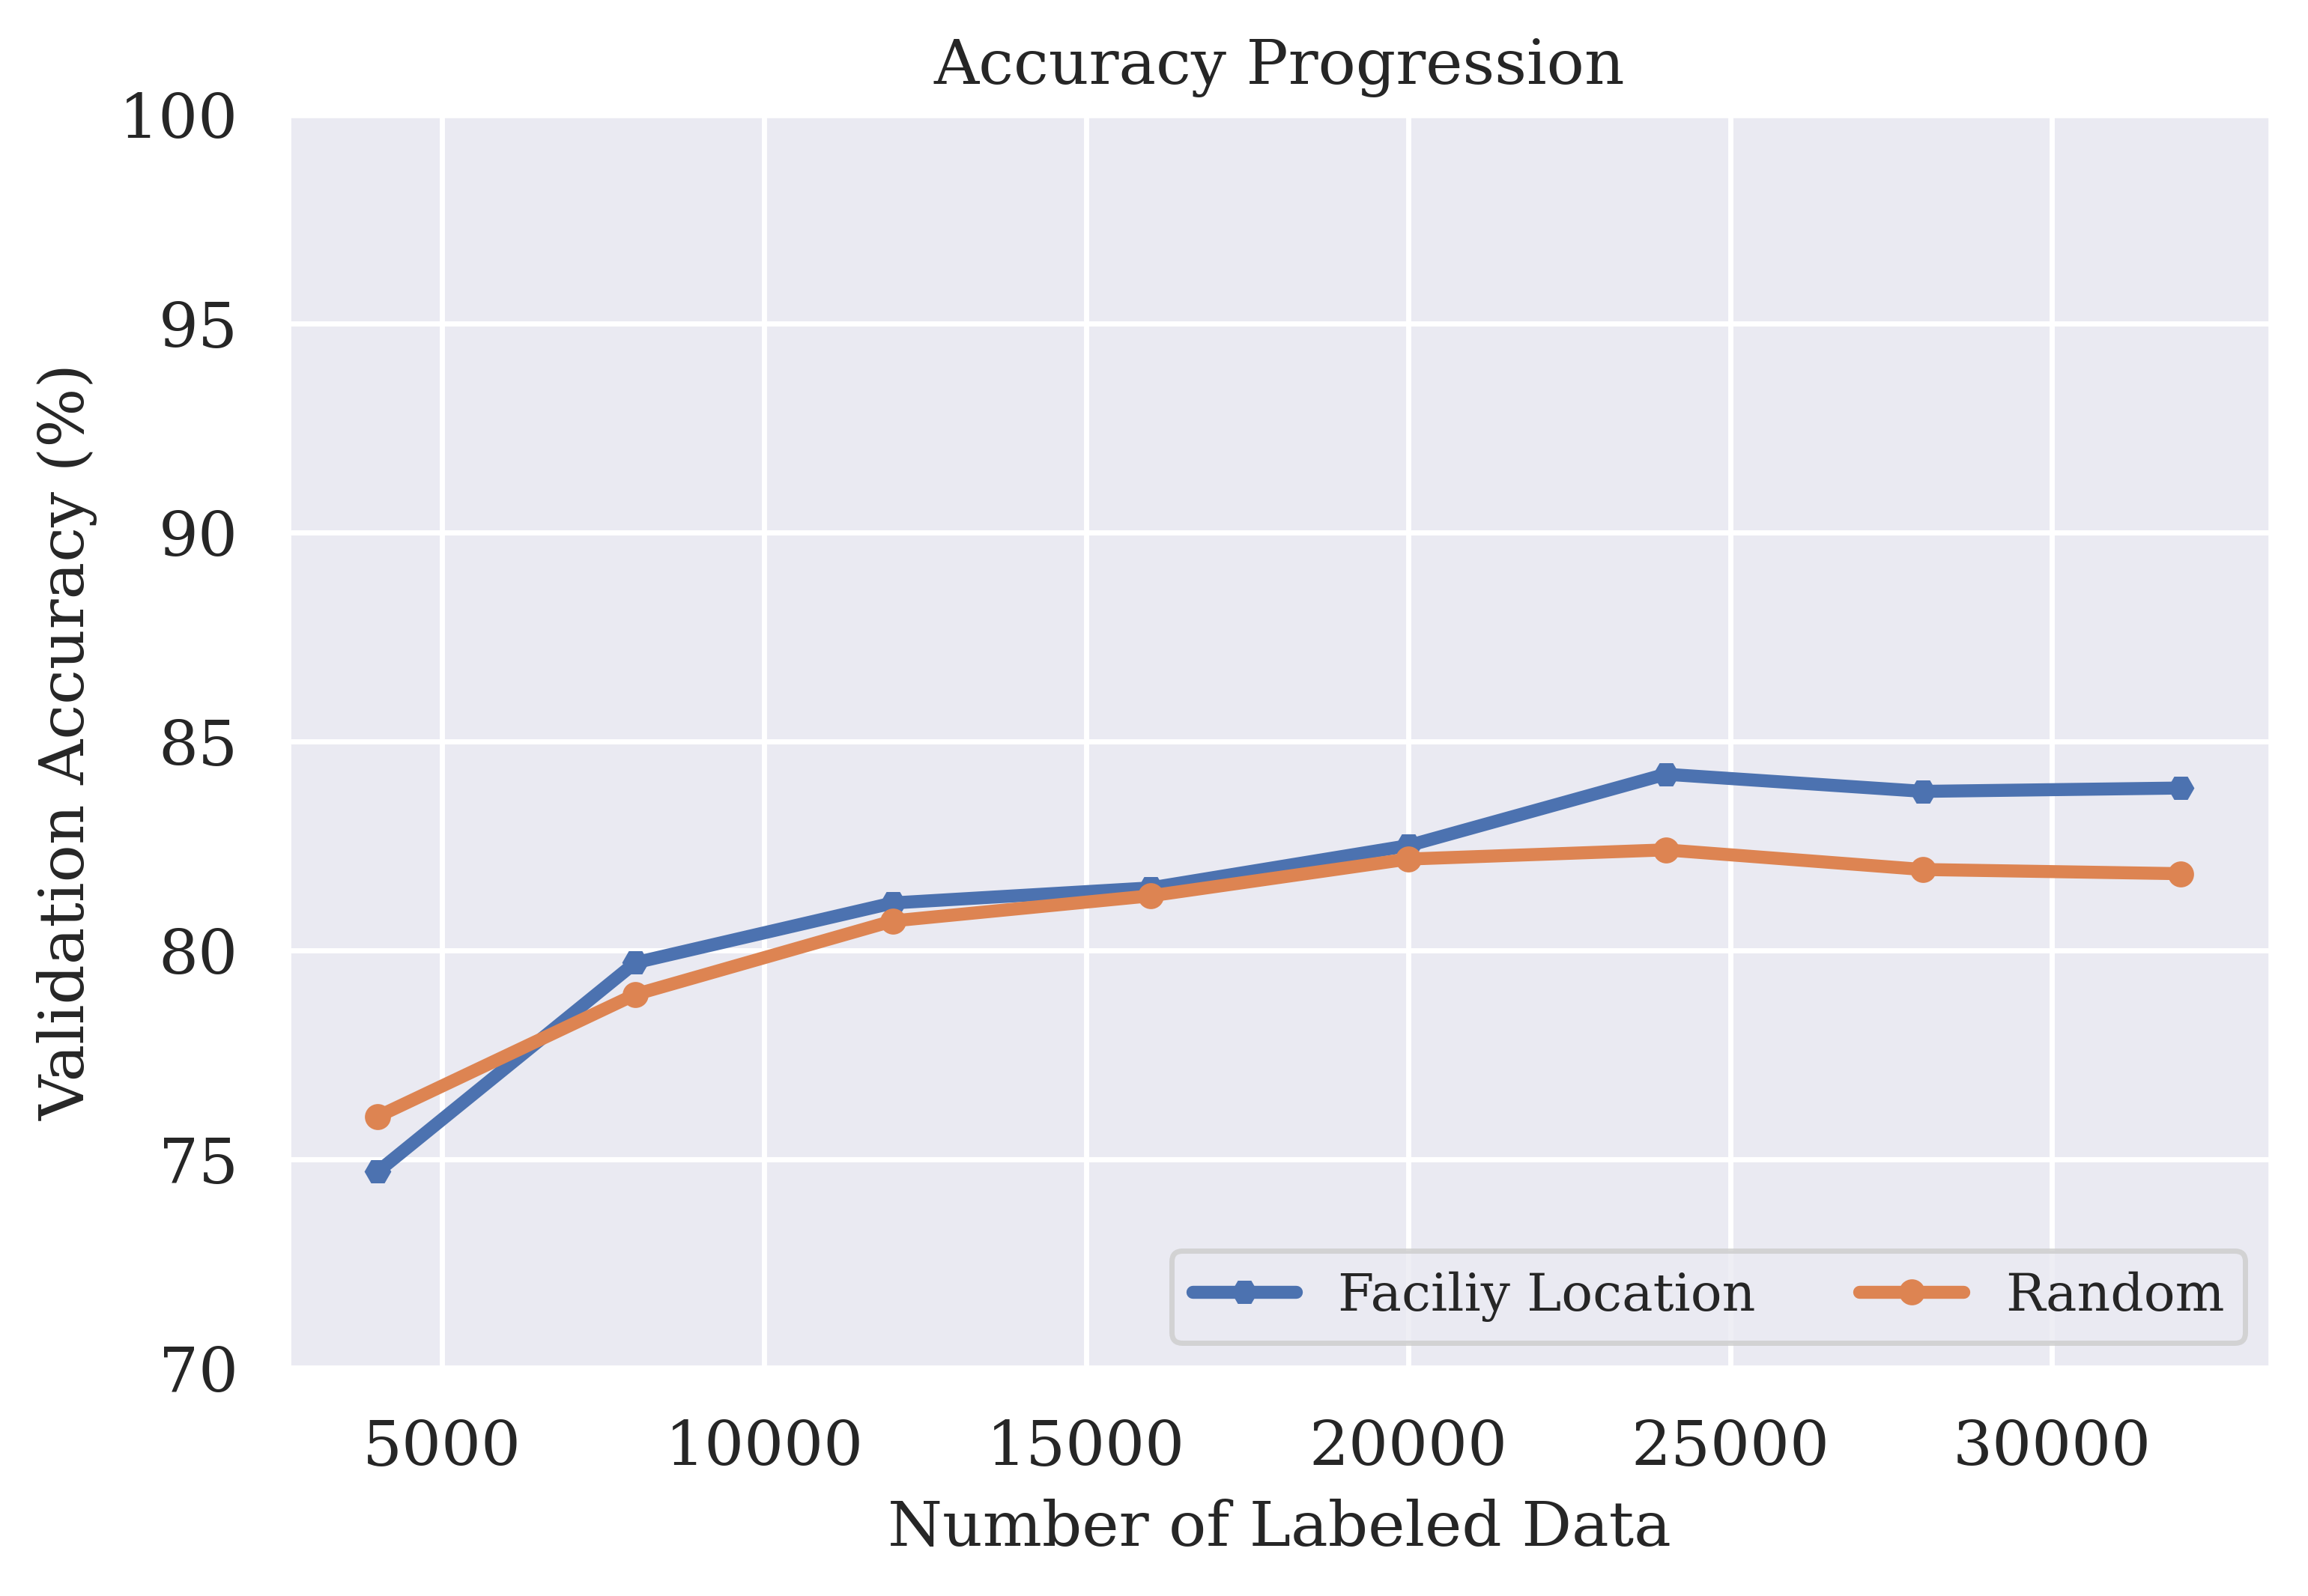
\includegraphics[width=\linewidth]{images/results_CAL/Facility_location_init.png}
    \caption[Initialization using Facility Location]{Comparison of validation accuracy for facility location initialization and random initialization. We use a batch size of 4000 and the combination of \gls{badge} and \gls{mas} for the experiments.}
    \label{fig:Evaluation:Results:CAL:FLinit}
\end{figure}


\subsubsection{Custom Replay approach}
\label{sec:Evaluation:Results:CAL:Replay}
In section \ref{sec:Methodology:ReplayStrategy} we propose a custom replay strategy for Continual Active Learning. The use of our replay strategy is motivated by the main finding of section \ref{sec:Evaluation:Results:CAL:ALCL}: the validation accuracy increases with an
increased batch size. In this set of experiments, we use the Active Learning strategy CoreSet and vary the batch size and the size of the replay buffer. Moreover, we investigate the effect of CoreSet selection in the replay buffer compared to random selection. We present our
results in figure \ref{fig:Evaluation:Results:CAL:Replay}. When varying the batch size and buffer size, we notice that increasing the buffer size and the batch size yields a higher validation accuracy. However, our replay strategy does not outperform the Naive approach when using
the same amount of training data (i.e. batch size + replay buffer size for the replay strategy and batch size for the Naive approach). To evaluate the importance of CoreSet selection in the buffer compression process, we compare the validation accuracy of our replay strategy
when using CoreSet selection and random selection. We notice that the validation accuracy remains largely the same for both buffer compression methods, apart from the last 15000 samples, where CoreSet selection outperforms random selection. \par

\begin{figure}[h]
    \centering
    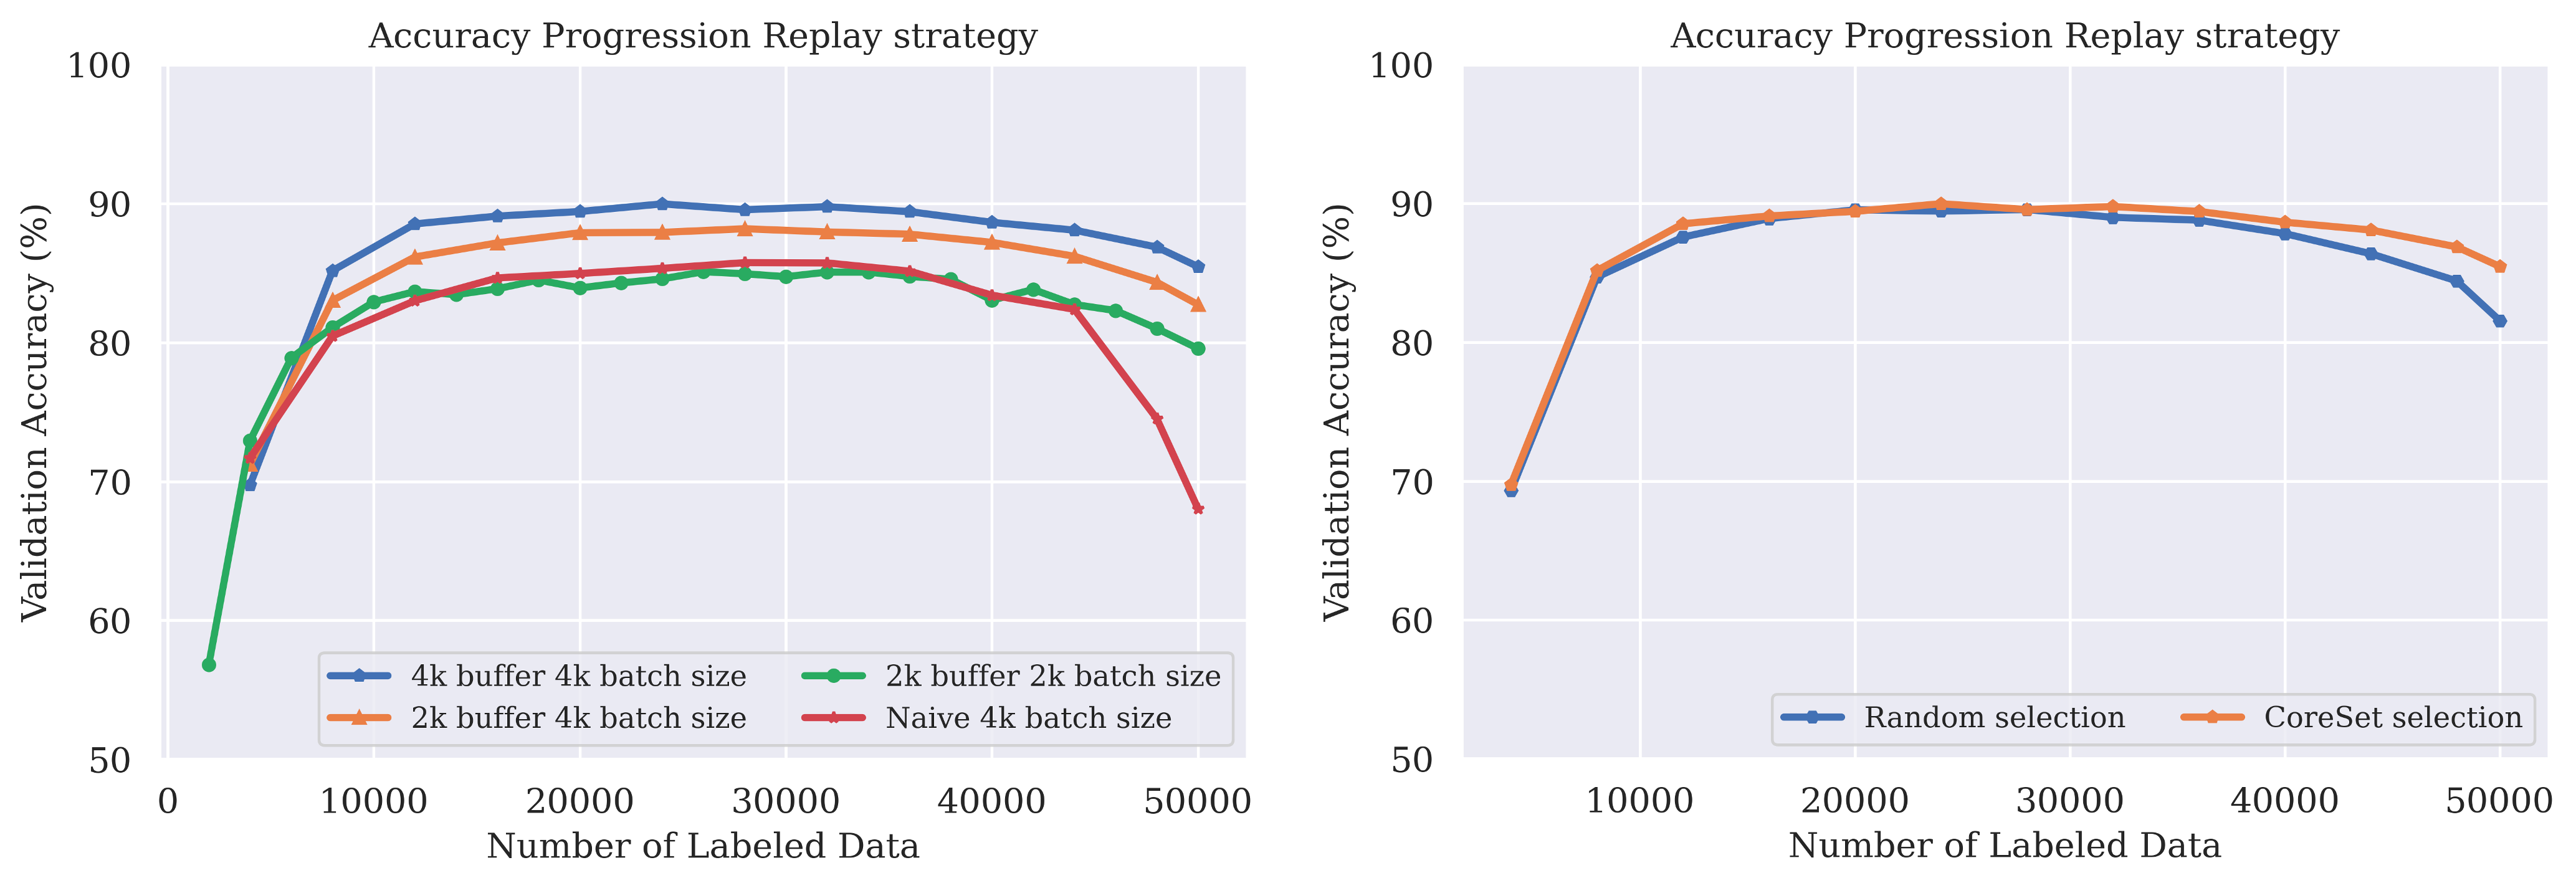
\includegraphics[width=\linewidth]{images/results_CAL/replay_CAL.png}
    \caption[Continual Active Learning Custom Replay strategy]{Left: Comparison of validation accuracy of our Replay strategy with different hyperparameters. Right: Comparison of validation accuracy of our Replay strategy when using different buffer compression approaches.
    In both runs, we use a batch size of 4000 and a replay buffer size of 4000.}
    \label{fig:Evaluation:Results:CAL:Replay}
\end{figure}

\subsection{Exemplar Rehearsal Continual Learning and Representation-based Active Learning}
\label{sec:Evaluation:Results:CAL:VAAL_AGEM}
Unsatisfied with the results from previous experiments, we decide to implement further Continual and Active Learning strategies. We perform an extensive literature search, investigating the suitability of representation-based Active Learning strategies and Continual Learning
strategies from the Exemplar Rehearsal category in the summary paper by Mundt et al. \cite{mundt2020wholistic}. The Active Learning strategy which we implement is \gls{vaal} \cite{sinha2019variational} and the Continual Learning strategy is \gls{a-gem} \cite{chaudhry2019continual}. We decide
to implement \gls{vaal} because it is the only representation-based Active Learning strategy which consistently performs better than random sampling. The reason why we choose to implement \gls{a-gem} as our Continual Learning strategy is that is one of the few Exemplar Rehearsal strategies
applicable to (Semi-) supervised Learning (many other strategies focus on Reinforcement Learning) while being computationally efficient and demonstrating strong performance in the experiments by Chaudhry et al. \cite{chaudhry2019continual} at the same time. \par
First, we analyze the performance of \gls{vaal} as an Active Learning strategy. We run \gls{vaal} with a batch size of 4000 and compare it to Random and CoreSet. We choose Random because it is the baseline for Active Learning strategies and CoreSet because it is among the best performing Active
we used before. The results can be found in the left plot in figure \ref{fig:Evaluation:Results:CAL:VAAL}. While \gls{vaal} outperforms random sampling by a large margin, it is itself outperformed by about the same margin by Coreset. To ensure that the results are not due to a
suboptimal hyperparameter choice, we run \gls{vaal} training VAE and Discriminator for 20 epochs in one run and 100 epochs in another. Because we are interested in the performance of \gls{vaal} in our Continual Active Learning setting, we use Continual Active Learning with a batch size of 4000
and the Continual Learning strategy Naive. We present the results of the experiment in the right plot of figure \ref{fig:Evaluation:Results:CAL:VAAL}. Surprisingly, the validation accuracy is marginally impacted by the training time of Generator and VAE. If anything, the validation
accuracy is higher when training for 20 epochs. \par

\begin{figure}[h]
    \centering
    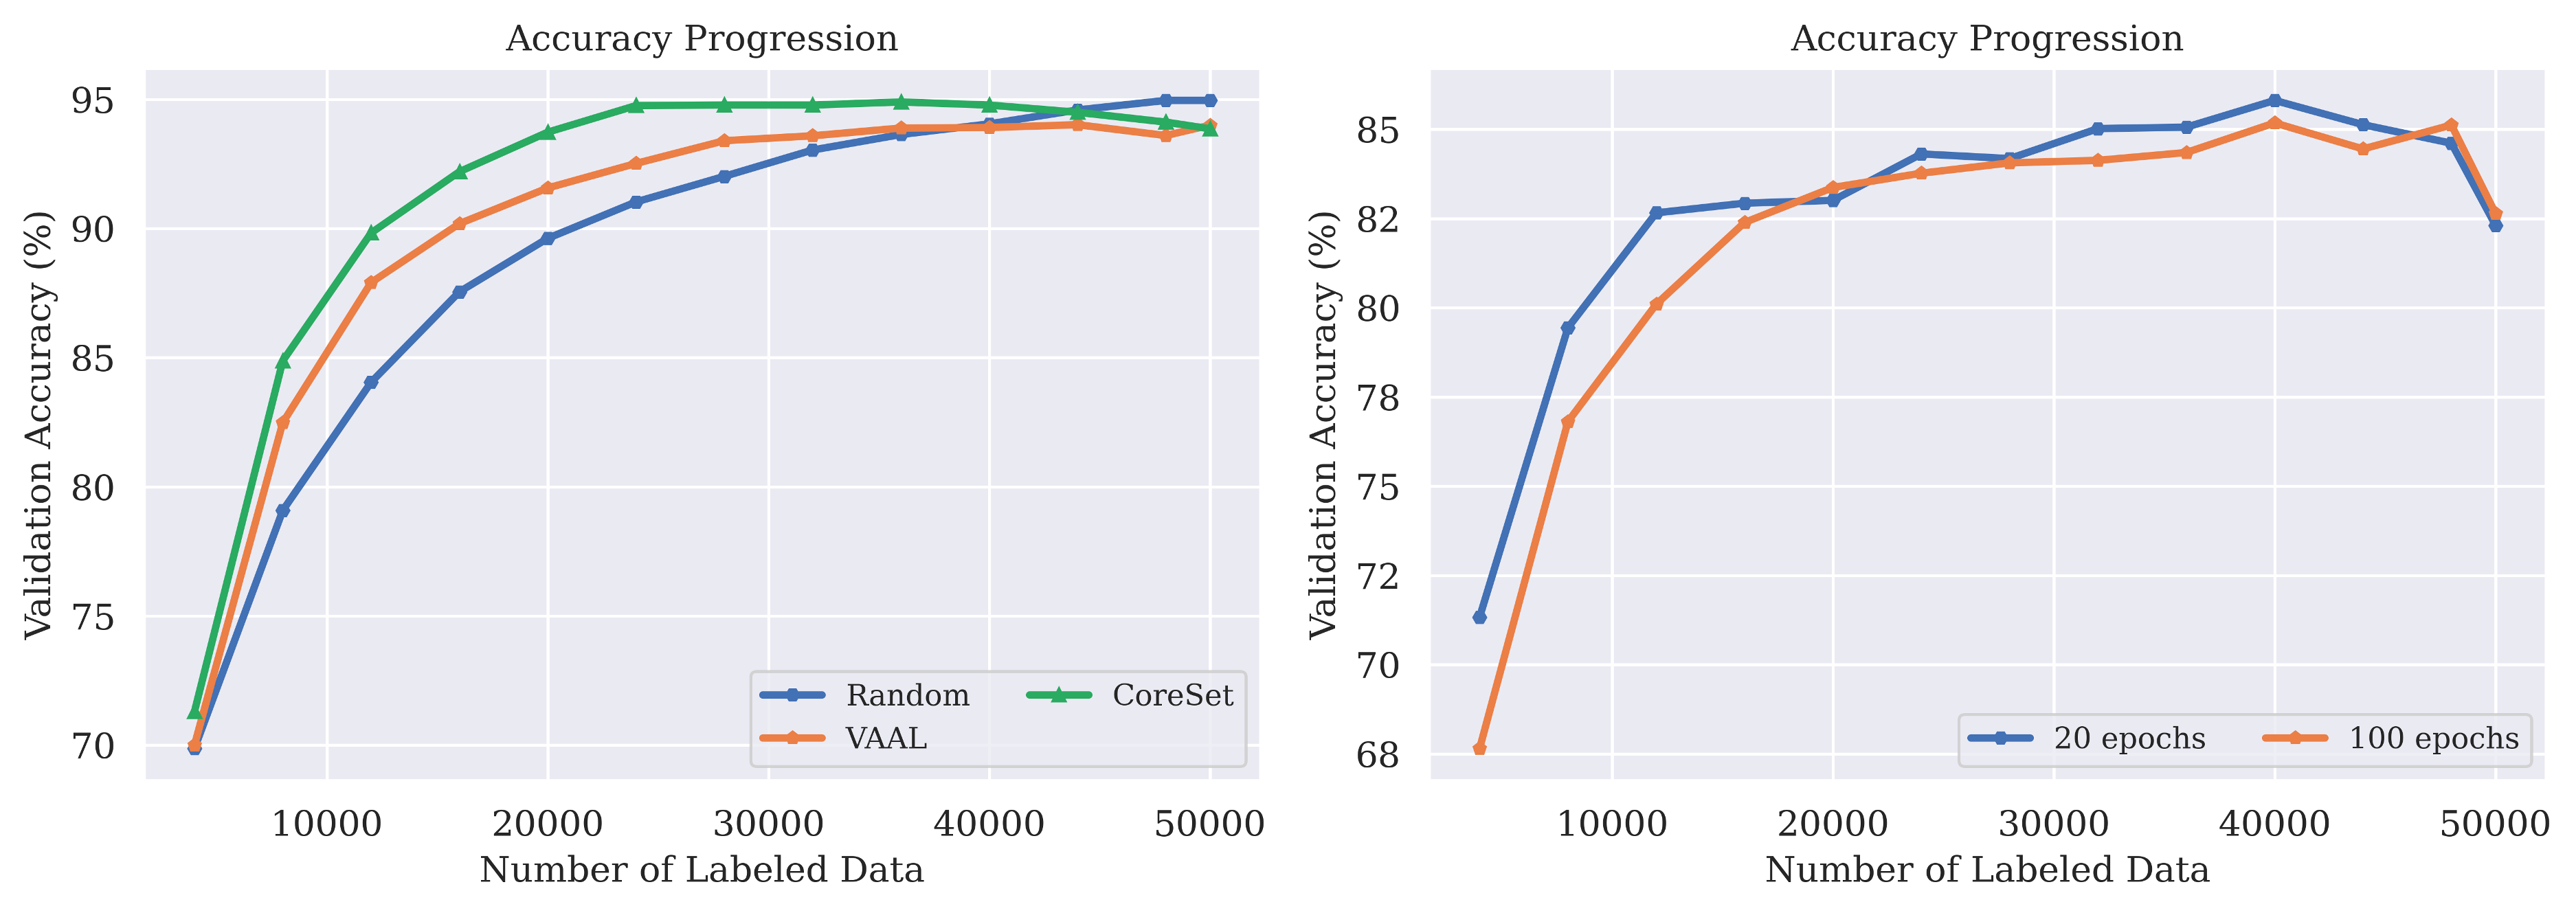
\includegraphics[width=\linewidth]{images/results_CAL/VAAL_plots.png}
    \caption[Continual Active Learning Custom Replay strategy]{Left: Comparison of validation accuracy of \gls{vaal} to the Active Learning strategies Random and CoreSet. We use a batch size of 4000 for the experiments. Right: Comparison of validation accuracy when varying the training 
    epochs for \gls{vae} and Discriminator. We use Continual Active Learning with the Naive approach as our Continual Learning strategy and a batch size of 4000.}
    \label{fig:Evaluation:Results:CAL:VAAL}
\end{figure}

Next, we experiment with \gls{a-gem}. \gls{a-gem} has two hyperparameters: $S$, which is the number of samples randomly drawn from the memory to compute the reference gradients and $P$ which is the number of data points stored to the memory from each task. We run \gls{a-gem} with the Active Learning
strategy \gls{lc} and a batch size of 2000. To assess the performance of \gls{a-gem}, we compare its validation accuracy to the Naive approach. We vary $S$ and $P$ and present our results in the right plot of figure \ref{fig:Evaluation:Results:CAL:AGEM}. The validation accuracy increases with
an increased $S$ and $P$ until about 12000 samples, after which the validation accuracy drops for all values of $S$ and $P$. \gls{a-gem} outperforms the Naive approach for the first 15000 samples, but is outperformed by Naive for the remainder of the experiment. \par
After investigating the influence of \gls{a-gem}'s hyperparameters, we compare the combination of \gls{vaal} and \gls{a-gem} to \gls{vaal} and Naive, using a batch size of 4000. The results are shown in the left plot of figure \ref{fig:Evaluation:Results:CAL:AGEM}. Although \gls{a-gem} performs worse than the Naive
approach when using the Active Learning strategy \gls{lc}, it outperforms the Naive approach when using \gls{vaal} as the Active Learning strategy. \par

\begin{figure}[h]
    \centering
    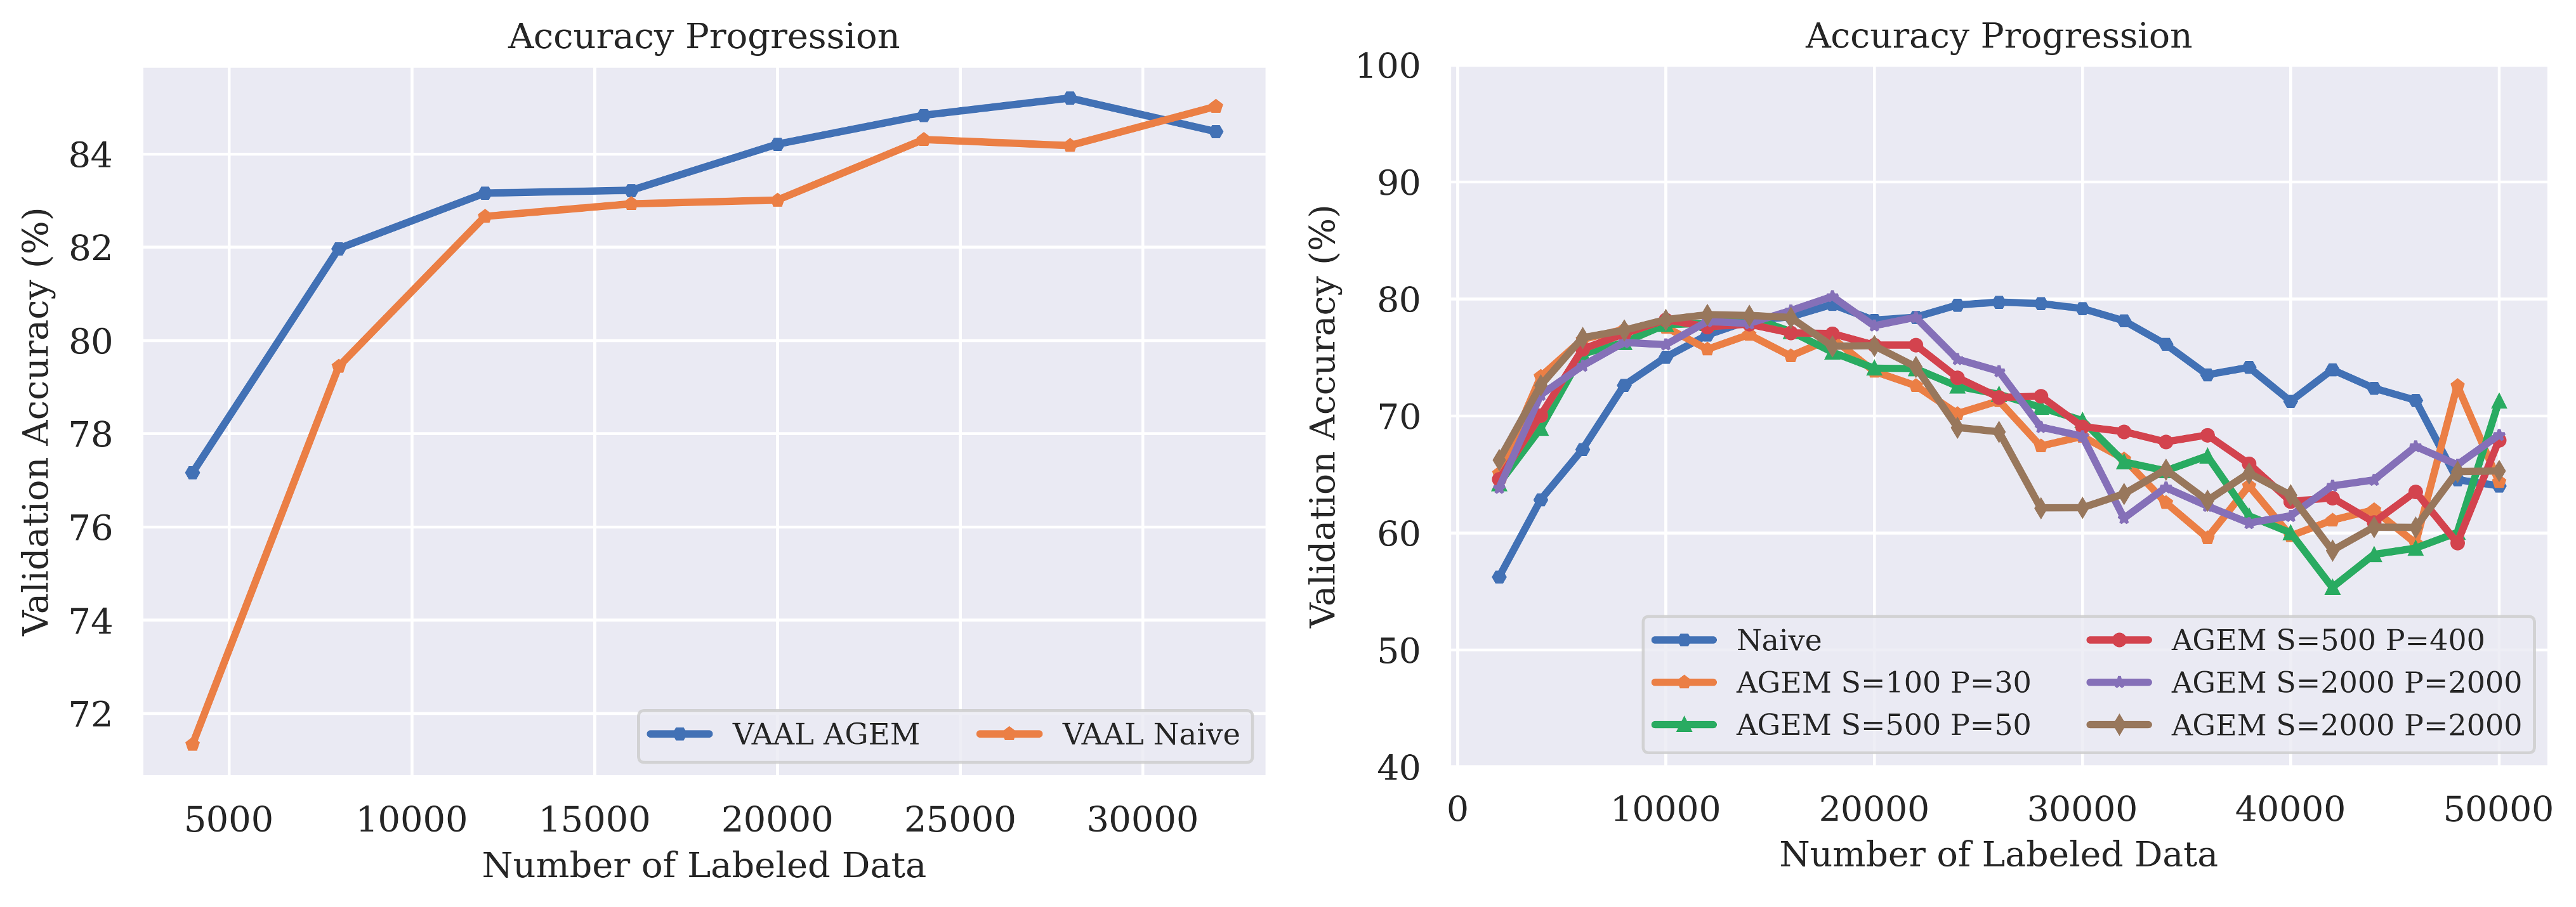
\includegraphics[width=\linewidth]{images/results_CAL/AGEM_plots.png}
    \caption[Continual Active Learning Custom Replay strategy]{Left: Comparison of validation accuracy of \gls{a-gem} to the Naive approach when using \gls{vaal} as the Active Learning strategy We use a batch size of 4000 for the experiments. Right: Comparison of validation accuracy of \gls{a-gem}
     to the Naive approach when using different values of $S$ and $P$. We use the Active Learning strategy \gls{lc} and a batch size of 2000 for the experiments.}
    \label{fig:Evaluation:Results:CAL:AGEM}
\end{figure}

\subsection{Continual Active Learning for Model Stealing}
\label{sec:Evaluation:Results:MS}
After extensively studying Continual Active Learning, we shift the focus of our experiments to Model Stealing. Since we build our work on the ActiveThief framework, we first evaluate the performance of the ActiveThief framework, including the influence of Model Architecture and
Thief Dataset as well as the difference between stealing a target model returning the predicted labeled and stealing a target model returning the softmax outputs of the final model layer. After experimenting with the ActiveThief framework, we evaluate the performance of our pro
-posed Continual Active Learning strategy for Model Stealing attacks. We perform the experiments on the MNIST, CIFAR-10 and CIFAR-100 datasets and end with a decisive insight on the effect of data augmentation for Model Stealing attacks. \par





\subsubsection{Model Stealing Attacks using Continual Active Learning}
\label{sec:Evaluation:Results:MS:CAL}

In this section, we evaluate the success of Model Stealing Attacks using Continual Active Learning. More specifically, we run Model Stealing Attacks with Continual Active Learning on the datasets MNIST, CIFAR-10 and CIFAR-100, using the Active Learning strategies
Random, \gls{lc}, \gls{bald}, \gls{badge} and CoreSet and the Continual Learning strategies Naive, \gls{ewc}, \gls{imm}, \gls{mas} and \gls{alasso}. Furthermore, we differentiate between receiving the softmax output of the target model and solely receiving the top1-label. We use the ActiveThiefConv3 model
as the target and substitute model and perform one model stealing attack for each combination of Active Learning, Continual Learning strategy and target model output. For the baseline runs, we use a batch size of 1000 with a total query budget of 20000. The query budget
is kept for the Continual Active Learning runs, but we increase the batch size to 2000. The numbers reported in the table represent the model agreement at the end of each experiment, i.e. after using up the query budget of 20000. Readers interested in the progression of the
model agreement across the experiments can find the respective plots in appendix \ref{sec:Appendix:Results}. As a baseline we use the Model Extraction using Active Learning with the strategies mentioned before. To evaluate both the Active Learning strategies and the Continual
Learning strategies, we compute the average over the model agreement of all Continual Learning strategies combined with a fixed Active Learning strategy and the average of all Active Learning strategies combined with a fixed Continual Learning strategy. These numbers are given
at the end of each column and row, respectively. The Active Learning strategy and the Continual Learning strategy with the highest average model agreement are highlighted in bold. \par
In the first set of experiments, we perform Model Stealing Attacks using Continual Active Learning with MNIST as our target model and train the substitute model on the softmax output of the target model. The results of this experiment can be found in table
\ref{fig:ModelStealingMNISTSoftmax}. In terms of model agreement, all Continual Active Learning attacks perform significantly worse than the baseline. The best performing attack is the combination of the Active Learning strategy \gls{bald} with the Continual Learning strategy
\gls{mas} with a model agreement of 67.84\% after a query budget of 20000. The best performing Active Learning strategy is \gls{bald} with an average model agreement of 52.52\% across all Continual Learning strategies whereas the best Continual Learning strategy is \gls{mas} with an average
model agreement of 57.73\%. While the Continual Learning strategies struggled to outperform the Naive approach in the classic Continual Active Learning setting, most of them outperform the Naive approach in the Model Stealing setting. The only exception to this is \gls{alasso} which
falls behind the other approaches significantly. \par 

\begin{table}[h]
    \centering
    \begin{tabular}{c | c c c c c | c } 
        \hline
        \diagbox[width=11em]{Active \\ Learning Strategy}{Continual Learning \\ Strategy} & Random & \gls{lc} & \gls{bald} & CoreSet & \gls{badge} & $\varnothing$\\ 
        \hline 
        Baseline & 87.91 & 82.39 & 83.64 & 91.22 & 79.68 & 84.97\\
        \hline
        Naive & 47.74 & 43.02 & 59.61 & 58.36 & 48.89 & 51.52\\
        \gls{ewc} &  59.26 & 53.67 & 59.18 & 56.13 & 50.28 & 55.7\\
        \gls{imm} & 48.18 & 62.95 & 49.71 & 63.43 & 58.76 & 56.61 \\
        \gls{mas} &  64.42 & 50.27 & 67.84 & 55.58 & 50.54 & \textbf{57.73}\\
        \gls{alasso} & 28.04 & 15.5 & 26.28 & 10.39 & 12.8 & 20.6\\
        \hline
        $\varnothing$ & 49.57 & 45.08 & \textbf{52.52} & 48.78 & 44.24 & \\
        \hline
    \end{tabular}
    \caption[Model agreement of Continual Learning strategies on MNIST using softmax output]{Comparison of Model Agreement (in \%) for Model Stealing Attacks using Continual Active Learning on the MNIST dataset. We use Model Stealing Attacks with Active Learning as a baseline.
    In this set of experiments, we use the softmax output of the target model to train the substitute model.}
    \label{fig:ModelStealingMNISTSoftmax}
\end{table}

Next, we change the output of the target model to solely return the top1-label and perform the same set of experiments. Table \ref{fig:ModelStealingMNISTLabel} shows the results of these experiments. While the model agreement compared to training with softmax output of the
target model has dropped significantly for the baseline strategies, we do not observed a similar phenomenon for the Continual Active Learning strategies. Nevertheless, we observe a large maring between the Model Agreement of the Active Learning strategies and the Model Agreement
of the Continual Active Learning strategies. However, the combination of \gls{bald} and Naive comes close to its baseline, demonstrating a Model Agreement of 69.18\% which is about 7 percentage points lower than the respective baseline. Overall, the Naive approach performs best with an
average Model Agreement of 51.29\% across all Active Learning strategies. Contrary to the previous setup, no Continual Learning strategy outperforms the Naive approach, with \gls{mas} coming closest. The best Active Learning strategy is \gls{bald} with an average Model Agreement of 55.73\%. \par 

\begin{table}[h]
    \centering
    \begin{tabular}{c | c c c c c | c} 
        \hline
        \diagbox[width=11em]{Active \\ Learning Strategy}{Continual Learning \\ Strategy} & Random & \gls{lc} & \gls{bald} & CoreSet & \gls{badge} & $\varnothing$ \\ 
        \hline 
        Baseline & 67.56 & 80.36 & 76.29 & 81.62 & 76.43 & 76.45\\
        \hline
        Naive & 43.44 & 58.84 & 69.18 & 44.88 & 40.12 & \textbf{51.29}\\
        \gls{ewc} &  46.76 & 47.3 & 52.36 & 36.84 & 44.73 & 45.6\\
        \gls{imm} & 47.07 & 10.43 & 58.71 & 51.0 & 47.0 & 42.84\\
        \gls{mas} & 50.52 & 46.79 & 49.51 & 44.96 & 49.47 & 48.25\\
        \gls{alasso} &  10.44 & 46.89 & 48.89 & 16.27 & 10.43 & 26.68\\
        \hline
        $\varnothing$ & 39.65 & 50.97 & \textbf{55.73} & 38.79 & 38.35\\
        \hline
    \end{tabular}
    \caption[Model agreement of Continual Learning strategies on MNIST using the predicted class label]{Comparison of Model Agreement (in \%) for Model Stealing Attacks using Continual Active Learning on the MNIST dataset. We use Model Stealing Attacks with Active Learning as a baseline.
    In this set of experiments, we use the predicted label of the target model to train the substitute model.}
    \label{fig:ModelStealingMNISTLabel}
\end{table}

We move on to the next dataset which is CIFAR-10. First, we perform Model Stealing attacks using the softmax output of the target model. Our results can be found in Table \ref{fig:ModelStealingCIFAR10Softmax}. Similar to our findings from the MNIST dataset, the Continual Active Learning
are outperformed by the Active Learning strategies, however the gap between is mostly consistent across combinations of Active and Continual Learning strategies at around 10 percentage points. \gls{alasso} is once again an exception to this, performing significantly worse than the other
Continual Learning strategies. The best Continual Active Learning strategy is \gls{ewc} with an average Model Agreement of 60.14\%. At the same time, \gls{ewc} is the only Continual Learning strategy to outperform the Naive approach, albeit the margin between the two is only 0.48 percentage points.
Overall, CoreSet is the most performant Active Learning strategy with an average model agreement of 54.12\% across all Continual Learning strategies. \par

\begin{table}[h]
    \centering
    \begin{tabular}{c | c c c c c | c} 
        \hline
        \diagbox[width=11em]{Active \\ Learning Strategy}{Continual Learning \\ Strategy} & Random & \gls{lc} & \gls{bald} & CoreSet & \gls{badge} & $\varnothing$\\ 
        \hline 
        Baseline & 71.58 & 70.04 & 71.96 & 71.45 & 71.44 & 71.29\\
        \hline
        Naive & 60.8 & 56.62 & 61.84 & 61.61 & 57.42 & 59.66 \\
        \gls{ewc} & 58.67 & 56.8 & 61.57 & 61.79 & 61.88 & \textbf{60.14}\\
        \gls{imm} & 60.78 & 52.24 & 60.32 & 61.39 & 56.98 & 58.34 \\
        \gls{mas} & 50.32 & 51.45 & 52.09 & 52.23 & 55.68 & 52.35\\
        \gls{alasso} & 17.26 & 24.87 & 28.24 & 33.59 & 32.93 & 27.38\\
        \hline
        $\varnothing$ & 49.57 & 48.4 & 52.81 & \textbf{54.12} & 52.98\\
        \hline
    \end{tabular}
    \caption[Model agreement of Continual Learning strategies on CIFAR-10 using softmax output]{Comparison of Model Agreement (in \%) for Model Stealing Attacks using Continual Active Learning on the CIFAR-10 dataset. We use Model Stealing Attacks with Active Learning as a baseline. In this set of experiments,
    we use the softmax output of the target model to train the substitute model.}
    \label{fig:ModelStealingCIFAR10Softmax}
\end{table}

In our next experiment setup, we use the predicted label of the target model to train the substitute model, again with CIFAR-10 as the target model dataset. We present the results of this set of experiments in Table \ref{fig:ModelStealingCIFAR10Label}. Overall,
the Model Agreement is lower than when training with the softmax output of the target model, which is in line with the experiments conducted on the MNIST dataset. The gap between the baseline and the Continual Learning strategies has remained the same however,
resting at around 10 percentage points. \gls{ewc} is again the best performing Continual Learning strategy, outperforming the Naive approach by a large margin this time around. \gls{imm} follows closely, also beating the Naive approach. The main reason for the large gap
between the Naive approach and \gls{ewc} as well as \gls{imm} is the poor performance of \gls{bald} and Naive. Surprised by the poor performance of this combination, we run it again and find that the results are consistent. \gls{mas} and \gls{alasso}, on the other hand, do not manage to
outperform the Naive approach. In terms of Active Learning strategies, CoreSet performs best with an average Model Agreement of 43.57\% across all Continual Learning strategies. \par

\begin{table}[h]
    \centering
    \begin{tabular}{c | c c c c c | c} 
        \hline
        \diagbox[width=11em]{Active \\ Learning Strategy}{Continual Learning \\ Strategy} & Random & \gls{lc} & \gls{bald} & CoreSet & \gls{badge} & $\varnothing$\\ 
        \hline 
        Baseline & 60.23 & 49.73 & 61.28 & 63.78 & 62.26 & 59.46\\
        \hline
        Naive & 49.84 & 30.03 & 10.18 & 48.44 & 45.25 & 36.75\\
        \gls{ewc} & 50.37 & 47.12 & 50.22 & 47.94 & 49.11 & \textbf{48.95} \\
        \gls{imm} & 49.84 & 44.25 & 43.55 & 49.64 & 48.22 & 47.1\\
        \gls{mas} & 45.76 & 33.27 & 36.87 & 39.98 & 40.24 & 32.02\\
        \gls{alasso} & 19.05 & 38.16 & 30.91 & 31.86 & 25.04 & 29.0\\
        \hline
        $\varnothing$ & 42.97 & 38.57 & 34.35 & \textbf{43.57} & 41.57\\
        \hline
    \end{tabular}
    \caption[Model agreement of Continual Learning strategies on CIFAR-10 using the predicted class label]{Comparison of Model Agreement (in \%) for Model Stealing Attacks using Continual Active Learning on the CIFAR-10 dataset. We use Model Stealing Attacks with Active
    Learning as a baseline. In this set of experiments, we use the predicted label of the target model to train the substitute model.}
    \label{fig:ModelStealingCIFAR10Label}
\end{table}

The final target model dataset which we test for our setup is CIFAR-100. Like in the previous experiments, we first test all combination of Continual and Active Learning strategies trained on the softmax output of the target model
and compare them to the baseline of Active Learning. An exception to this are all experiments involving the Active Learning strategy \gls{badge}. We found the estimated runtime of \gls{badge} using ActiveThiefConv as our substitute model and SmallImagenet as our thief dataset
to be in excess of 40 days on our hardware, which is why we were unable to deliver results for this combination. The results for the remaining combinations from this set of experiments can be found in table \ref{fig:ModelStealingCIFAR100Softmax}.
Across the board, Model Agreement is significantly lower than in our previous experiments. The gap between the baseline and the Continual Learning strategies has decreased in absolute terms but increased in relative terms. Like in our previous experiments, \gls{ewc} outperforms
the remaining Continual Learning strategies, and it is one of two Continual Learning strategies which manage to outperform the Naive approach. The other strategy is \gls{imm}, which puts on a performance in between \gls{ewc} and the Naive approach. \gls{mas} follows behind the Naive approach
and \gls{alasso} is left behind once again. The best Active Learning strategy is CoreSet, which outperforms \gls{bald} by 0.57 percentage points. \par

\begin{table}[h]
    \centering
    \begin{tabular}{c | c c c c | c} 
        \hline
        \diagbox[width=11em]{Active \\ Learning Strategy}{Continual Learning \\ Strategy} & Random & \gls{lc} & \gls{bald} & CoreSet & $\varnothing$\\ 
        \hline 
        Baseline & 25.43 & 26.92 & 28.01 & 27.48 & 26.96 \\
        \hline
        Naive & 18.46 & 18.48 & 16.8 & 17.69 & 17.86\\
        \gls{ewc} & 19.45 & 17.46 & 20.67 & 19.98 & \textbf{19.39}\\
        \gls{imm} & 18.16 & 17.9 & 20.39 & 18.75 & 18.8\\
        \gls{mas} & 15.75 & 14.85 & 14.72 & 15.45 & 15.19\\
        \gls{alasso} & 5.2 & 4.95 & 6.7 & 10.24 & 6.77\\
        \hline
        $\varnothing$ & 15.4 & 14.73 & 15.85 & \textbf{16.42}\\
        \hline
    \end{tabular}
    \caption[Model agreement of Continual Learning strategies on CIFAR-100 using softmax output]{Comparison of Model Agreement (in \%) for Model Stealing Attacks using Continual Active Learning on the CIFAR-100 dataset. We use Model Stealing Attacks with Active Learning as a baseline.
    In this set of experiments, we use the softmax output of the target model to train the substitute model.}
    \label{fig:ModelStealingCIFAR100Softmax}
\end{table}

Finally, we compute the Model Agreement across multiple combinations of Continual Learning and Active Learning strategies using the predicted label of the target model and CIFAR-100 as our target model dataset. As in the previous set of experiments, we omit the results of
the Active Learning strategy \gls{badge}. Compared to training on the softmax output of the target model, the model agreement has disproportionally decreased for the Continual Learning strategies. While the baseline strategies boast a Model Agreement of 20.42\% on average, the
best Continual Learning strategy, which is \gls{imm}, manages to achieve a Model Agreement of 8.07\% on average. \gls{imm} significantly outperforms both the Naive approach and \gls{ewc}, which demonstrate almost identical performance. We were surprised by the poor performance of \gls{ewc} and \gls{bald},
which is why we conducted this experiment one more time, however we achieved similar results. The remaining Continual Learning strategies, \gls{mas} and \gls{alasso}, perform worse than the Naive approach. Remarkably, \gls{alasso} outperforms \gls{mas}, making this the only set of experiments in which
\gls{alasso} is not the worst performing Continual Learning strategy. Another surprise is the performance of the Random Active Learning strategy, which outperforms the remaining Active Learning strategies. CoreSet, which demonstrated strong performance in previous experiments, falls behind
Random and \gls{lc}, outperforming only \gls{bald} by about one percentage point. \par

\begin{table}[h]
    \centering
    \begin{tabular}{c | c c c c | c} 
        \hline
        \diagbox[width=11em]{Active \\ Learning Strategy}{Continual Learning \\ Strategy} & Random & \gls{lc} & \gls{bald} & CoreSet & $\varnothing$\\ 
        \hline 
        Baseline & 21.65 & 19.5 & 19.64 & 20.9 & 20.42\\
        \hline
        Naive & 7.93 & 7.63 & 4.98 & 4.82 & 6.34\\
        \gls{ewc} & 8.79 & 6.55 & 2.07 & 7.77 & 6.3\\
        \gls{imm} & 8.59 & 8.44 & 7.18 & 8.05 & \textbf{8.07}\\
        \gls{mas} & 5.37 & 5.44 & 5.3 & 4.52 & 5.16\\
        \gls{alasso} & 5.28 & 6.11 & 5.72 & 5.51 & 5.66\\
        \hline
        $\varnothing$ & \textbf{7.19} & 6.83 & 5.05 & 6.13 \\
        \hline
    \end{tabular}
    \caption[Model agreement of Continual Learning strategies on CIFAR-100 using the predicted class label]{Comparison of Model Agreement (in \%) for Model Stealing Attacks using
    Continual Active Learning on the CIFAR-100 dataset. We use Model Stealing Attacks with Active Learning as a baseline. In this set of experiments,
    we use the predicted label of the target model to train the substitute model.}
    \label{fig:ModelStealingCIFAR100Label}
\end{table}

After having conducted our experiments with the Continual Learning strategies Naive, \gls{ewc}, \gls{mas}, \gls{imm} and \gls{alasso} as well as the Active Learning strategies
Random, \gls{bald}, \gls{lc}, CoreSet and \gls{badge}, we test the combination of the Active Learning strategy \gls{vaal} with the Continual Learning strategy \gls{a-gem}. We motivate
this experiment by the performance of \gls{vaal} and \gls{a-gem} in the classic Continual Learning setup, given in Figure \ref{sec:Evaluation:Results:CAL:VAAL_AGEM}.
The experiments are performed in the same manner as the previous experiments in this section. To evaluate the performance of \gls{vaal} and \gls{a-gem}, we compare
the results to the best performing Active Learning strategy, CoreSet, and the combination of the best performing Continual Learning strategy and the
most performant Active Learning strategy, which are \gls{ewc} and CoreSet, respectively. The results of the comparison are given in Table 
\ref{fig:ModelStealingVAALAGEM}. We present the progression in Model Agreement with \gls{vaal} and \gls{a-gem} in Appendix \ref{sec:Appendix:Results}. While \gls{vaal}
and \gls{a-gem} cannot keep up with the performance of the baseline, just as all Continual Active Learning approaches, it performs on par with CoreSet and \gls{ewc},
outperforming them in 3 out of 6 experiments while being outperformed in the remaining 3 experiments. \par
\begin{table}[h]
    \centering
    \begin{tabular}{c c c c c c c} 
        \hline
        & \multicolumn{2}{c}{MNIST} & \multicolumn{2}{c}{CIFAR-10} & \multicolumn{2}{c}{CIFAR-100} \\ 
        \cline{2-7} Attack strategy & Softmax & Label & Softmax & Label & Softmax & Label \\
        \hline 
        \gls{vaal} \gls{a-gem} & 52.54 & 53.8 & 61.48 & 50.5 & 18.29 & 8.77\\
        CoreSet \gls{ewc} & 56.13 & 36.84 & 61.79 & 47.94 & 19.98 & 7.77 \\
        Coreset Baseline & 90.65 & 77.58 & 71.61 & 61.68 & 27.52 & 20.96\\
        \hline
    \end{tabular}
    \caption[Comparison of Model Agreement using \gls{vaal} and \gls{a-gem}]{Comparison of Model Agreement (in \%) for Continual Active Learning using \gls{vaal}
     and \gls{a-gem}, CoreSet and \gls{ewc} as well as the CoreSet Baseline}
    \label{fig:ModelStealingVAALAGEM}
\end{table}

We close the evaluation section with a surprising finding regarding the effect of data augmentation on the success of Model Stealing Attacks. While
we managed to reproduce the findings of Pal et al. for CIFAR-10, we failed to do so for MNIST. Since multiple training hyperparameters of the experiments
presented in ActiveThief were not disclosed by the authors, we experiment with different combinations of hyperparameters, including varying the optimizer,
the learning rate, the number of training epochs, the batch size and switching between cold start and warm start for Active Learning. Sadly, we were still
not able to reproduce the results of ActiveThief on MNIST. After conducting the experiments presented above, we decided to investigate another hyperparameter:
training with or without data augmentation. For this set of experiments, we leave all hyperparameters equal to the previous experiments, apart from the data
augmentation. It is important to note here that we do or do not use data augmentation on the thief dataset, not on the target model dataset. Training the
target model is always done using data augmentation. We perform the same model stealing attacks as before, using MNIST and CIFAR-10 as target model dataset
and present the results in figure \ref{fig:Evaluation:Results:CAL:EffectAugmentation}. When performing Model Stealing Attacks without data augmentation on
CIFAR-10, we notice that Model Agreement, both for Active Learning and Continual Active Learning, is significantly lower than when using data augmentation.
In this scenario, Continual Active Learning with data augmentation performs on par with Active Learning without data augmentation. However, when using MNIST
as target model dataset, the results are reversed. Here, Model Agreement is significantly lower when using data augmentation. More importantly Continual
Active Learning without data augmentation shows performance comparable to Active Learning with data augmentation. \par

\begin{figure}[h]
    \centering
    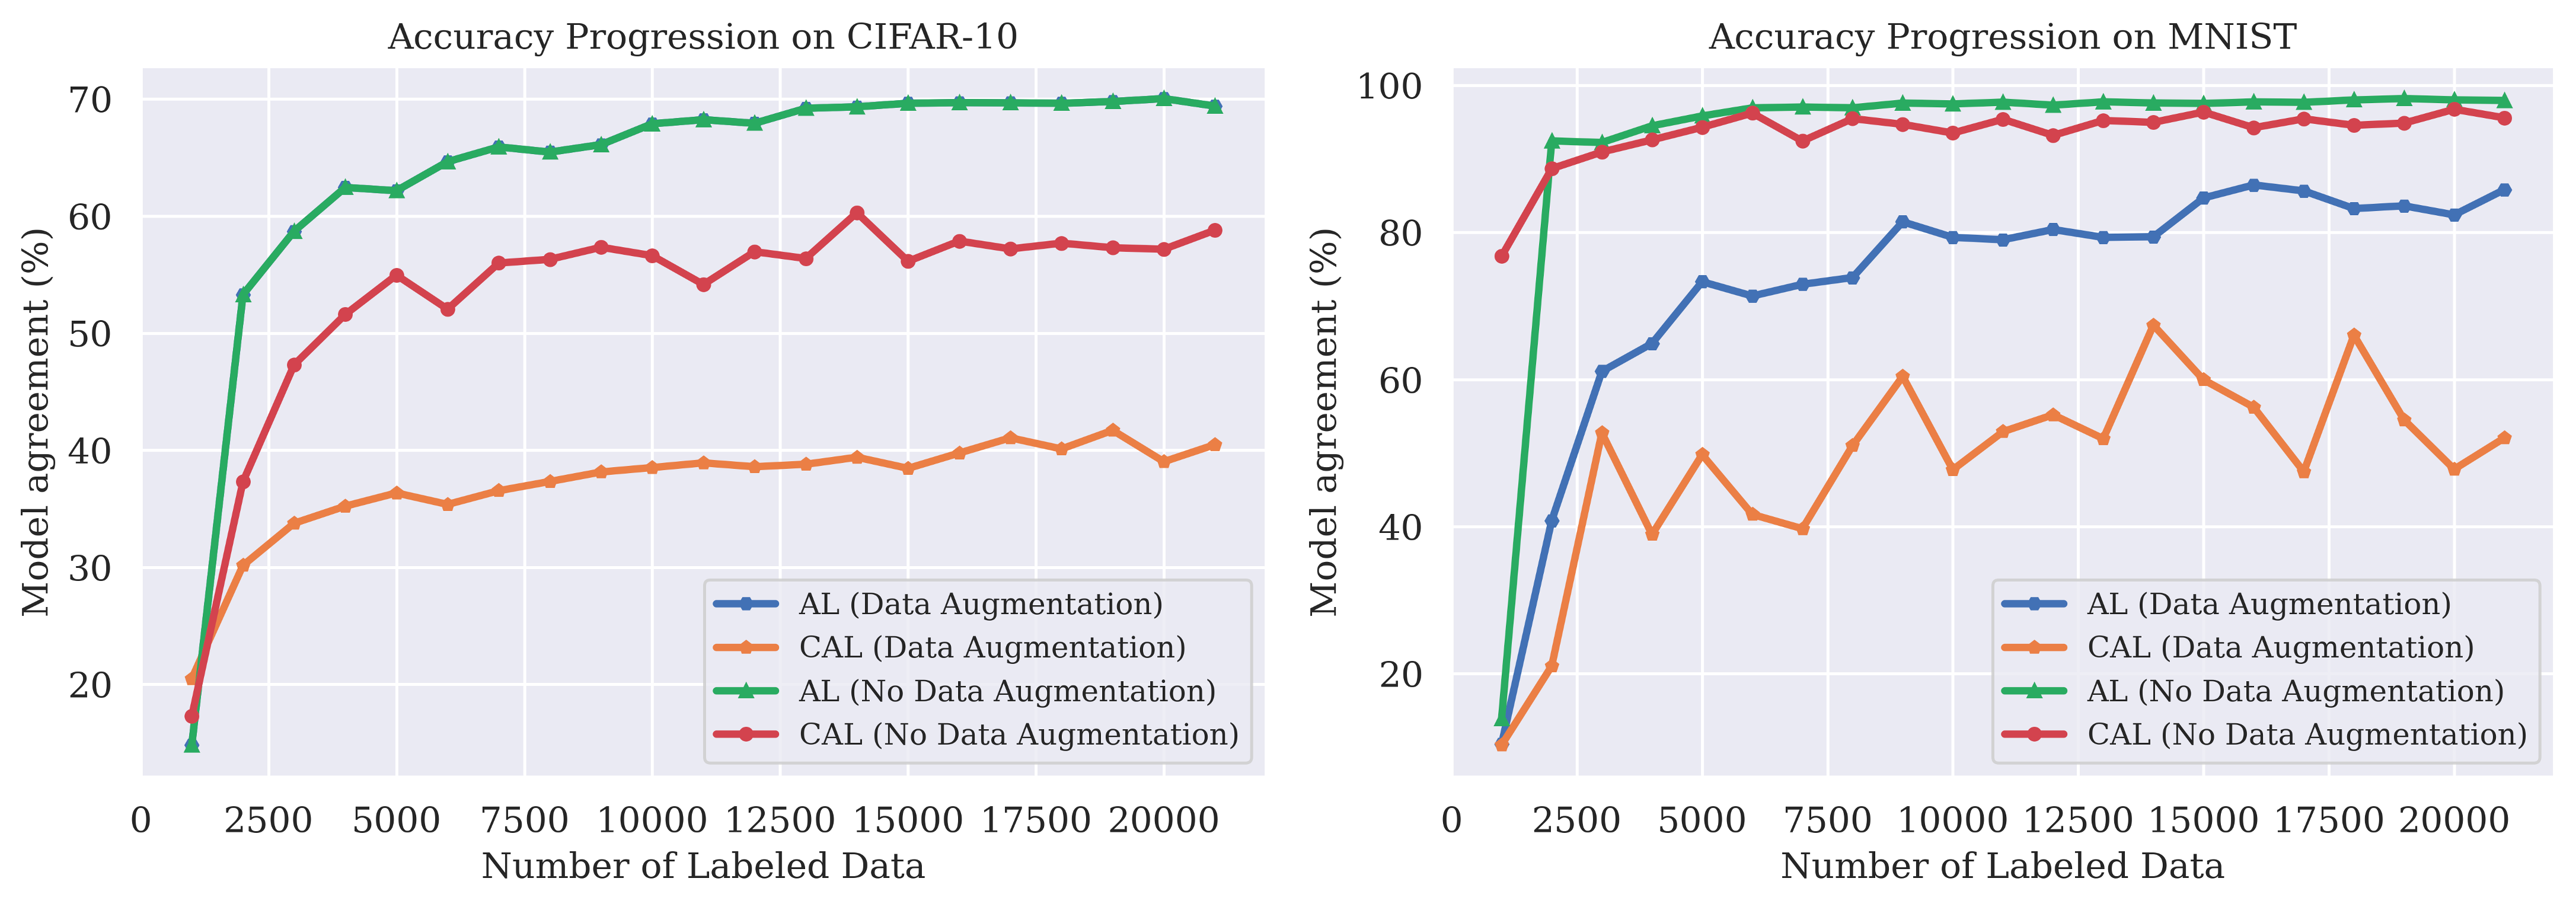
\includegraphics[width=\linewidth]{images/results_CALMS/effect_data_augmentation.png}
    \caption[Effect of Data Augmentation on the success of Model Stealing Attacks]{Comparison of Model Agreement when using different data augmentation
    techniques. For Active Learning we use a batch size of 1000 and for Continual Active Learning we use a batch size of 2000. Left: Experiments with
    the target model dataset CIFAR-10. Right: Experiments with the target model dataset MNIST.}
    \label{fig:Evaluation:Results:CAL:EffectAugmentation}
\end{figure}
